\documentclass[10pt,letterpaper]{article}
\usepackage[top=1in,left=1in,right=1in, bottom=1in]{geometry}

% amsmath and amssymb packages, useful for mathematical formulas and symbols
\usepackage{amsmath,amssymb}

% textcomp package and marvosym package for additional characters
\usepackage{textcomp,marvosym}

% line numbers
\usepackage[right]{lineno}

% easier turning on/off of includegraphics
\usepackage{ifthen}
\newboolean{includefigs}
\setboolean{includefigs}{true} % true/false


% ligatures disabled
\usepackage[nopatch=eqnum]{microtype}
\DisableLigatures[f]{encoding = *, family = * }

% Bold the 'Figure #' in the caption and separate it from the title/caption with a period
% Captions will be left justified
\usepackage[aboveskip=1pt,labelfont=bf,labelsep=period,justification=raggedright,singlelinecheck=off]{caption}
\renewcommand{\figurename}{Fig}

% Remove this for final submission, do not include graphics
\usepackage{graphicx} % Required for inserting images
\renewcommand{\figurename}{Fig S.D.}

\usepackage{datatool}
\DTLsetseparator{,}% Set the separator between the columns.
% todo add statistics file directly into this document
\DTLloaddbtex{\mydata}{../../output/statistics.dbtex}
\newcommand{\var}[1]{\DTLfetch{\mydata}{labels}{#1}{vals}}


\title{Quantifying prevalence and risk factors of HIV multiple infection in Uganda from population-based deep-sequence data}

\begin{document}
%TITLE_VPSACE

% Title must be 250 characters or less.
\begin{flushleft}

{\Large\textbf\newline{Quantifying prevalence and risk factors of HIV multiple infection in Uganda from population-based deep-sequence data \\ \medskip \large Supplementary File 4: Bayesian model fit diagnostics} 
%
%
% Please use "sentence case" for title and headings (capitalize only the first word in a title (or heading), the first word in a subtitle (or subheading), and any proper nouns).
}
\newline
% Insert author names, affiliations and corresponding author email (do not include titles, positions, or degrees).
\\
Michael A. Martin\textsuperscript{1,$\dagger$},
Andrea Brizzi\textsuperscript{2},
Xiaoyue Xi\textsuperscript{2,3},
Ronald Moses Galiwango\textsuperscript{4},
Sikhulile Moyo\textsuperscript{5,6},
Deogratius Ssemwanga\textsuperscript{7,8}
Alexandra Blenkinsop\textsuperscript{2},
Andrew D. Redd\textsuperscript{9,10,11},
Lucie Abeler-Dörner\textsuperscript{12},
Christophe Fraser\textsuperscript{12},
Steven J. Reynolds\textsuperscript{4,9,10},
Thomas C. Quinn\textsuperscript{4,9,10},
Joseph Kagaayi\textsuperscript{4,13},
David Bonsall\textsuperscript{14},
David Serwadda\textsuperscript{4},
Gertrude Nakigozi\textsuperscript{4},
Godfrey Kigozi\textsuperscript{4},
M. Kate Grabowski\textsuperscript{1,4,15,$\dagger$},
Oliver Ratmann\textsuperscript{2,$\dagger$},
with the PANGEA-HIV Consortium and the Rakai Health Sciences Program
\\
\bigskip
\textbf{1} Department of Pathology, Johns Hopkins School of Medicine, Baltimore, MD, USA
\\
\textbf{2} Department of Mathematics, Imperial College London, London, United Kingdom
\\
\textbf{3} Medical Research Council Biostatistics Unit, University of Cambridge, Cambridge, UK \\

\textbf{4} Rakai Health Sciences Program, Kalisizo, Uganda \\

\textbf{5} Botswana Harvard AIDS Institute Partnership, Botswana Harvard HIV Reference Laboratory, Gaborone, Botswana \\

\textbf{6} Harvard T.H. Chan School of Public Health, Boston, MA, USA \\

\textbf{7} Medical Research Council/Uganda Virus Research Institute and London School of Hygiene and Tropical Medicine Uganda Research Unit, Entebbe, Uganda \\

\textbf{8} Uganda Virus Research Institute, Entebbe, Uganda \\

\textbf{9} Department of Medicine, Johns Hopkins School of Medicine, Baltimore, MD, USA
\\
\textbf{10} Division of Intramural Research, National Institute of Allergy and Infectious Diseases, National Institutes of Health, Bethesda, MD, USA
\\
\textbf{11} Institute of Infectious Disease and Molecular Medicine, University of Cape Town, Cape Town, South Africa
\\
\textbf{12} Pandemic Sciences Institute, Nuffield Department of Medicine, University of Oxford, Oxford, UK \\

\textbf{13} Makerere University School of Public Health, Kampala, Uganda \\

\textbf{14} Wellcome Centre for Human Genetics, Nuffield Department of Medicine, University of Oxford, Oxford, UK \\

\textbf{15} Department of Epidemiology, Johns Hopkins Bloomberg School of Public Health, Baltimore, MD, USA \\
\bigskip

% Use the asterisk to denote corresponding authorship and provide email address in note below.
$\dagger$ Corresponding authors mmart108@jhmi.edu, mgrabow2@jhu.edu, oliver.ratmann@imperial.ac.uk 
\end{flushleft}
\newpage
\listoffigures
\newpage
% base simulation
\begin{figure}[!ht]
 \ifthenelse{\boolean{includefigs}}{\includegraphics[width=1\textwidth]{../../figures/base_simulation_base_trace.pdf}}{}
\caption{{\bf MCMC trace plots for parameters in base model fit to simulated data with partial sequencing success and no false positive or false negative multiple subgraph windows.} Independent chains are shown in shades of grey. Warm-up iterations are excluded. MI = multiple infection. VL = viral load (log\textsubscript{10} copies/mL) standardized to mean = 0 and std. dev = 1. Std. dev. = standard deviation.}
\end{figure}

\begin{figure}[!ht]
 \ifthenelse{\boolean{includefigs}}{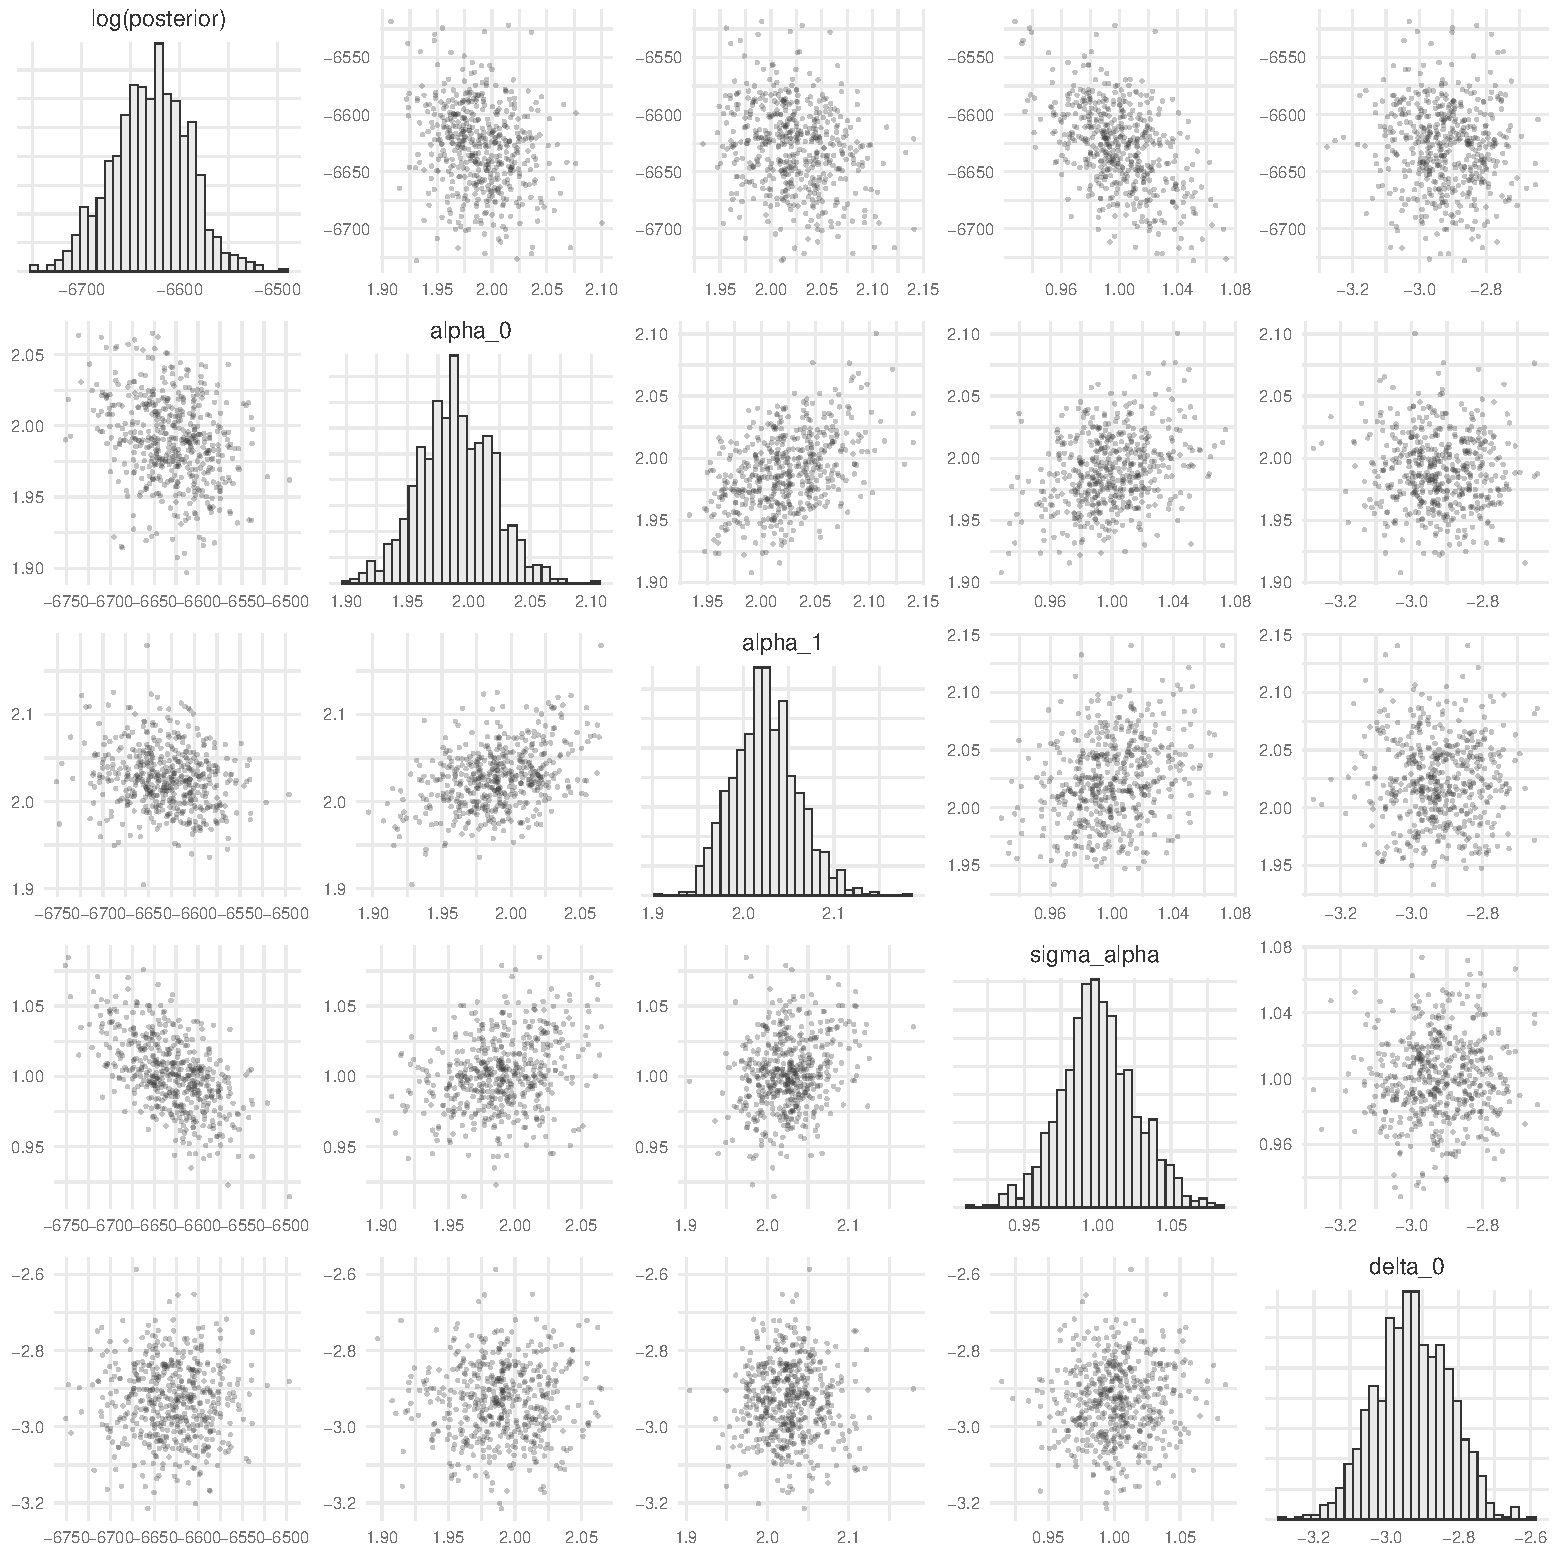
\includegraphics[width=1\textwidth]{../../figures/base_simulation_base_pairs.pdf}}{}
\caption{{\bf MCMC pairs plots for parameters in base model fit to simulated data with partial sequencing success and no false positive or false negative multiple subgraph windows.} Independent chains are shown in shades of grey. Warm-up iterations are excluded. Includes a sample of 250 iterations per chain. MI = multiple infection.}
\end{figure}

\begin{figure}[!ht]
 \ifthenelse{\boolean{includefigs}}{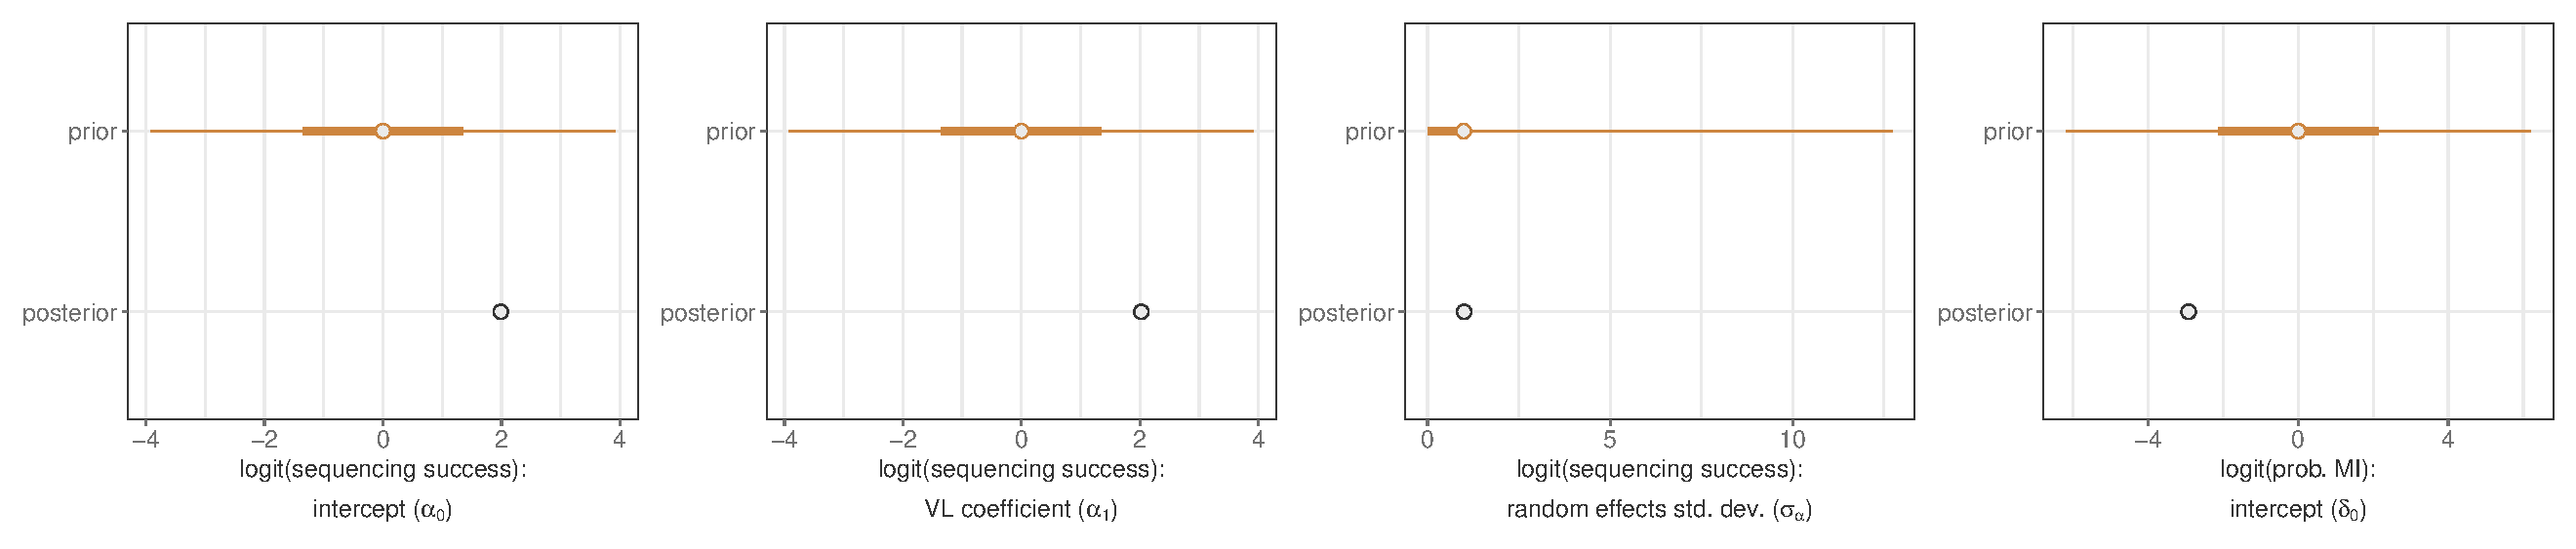
\includegraphics[width=1\textwidth]{../../figures/base_simulation_base_prior.pdf}}{}
\caption{{\bf Comparison of posterior and prior distributions of parameters in base model fit to simulated data with partial sequencing success and no false positive or false negative multiple subgraph windows.} Median is plotted as the central estimate and horizontal bars extend to the 95\% and 50\% HPD. Some horizontal bars do not extend beyond the central point. Warm-up iterations are excluded. MI = multiple infection. VL = viral load (log\textsubscript{10} copies/mL) standardized to mean = 0 and std. dev = 1. Std. dev. = standard deviation. }
\end{figure}

% full simulation
\begin{figure}[!ht]
 \ifthenelse{\boolean{includefigs}}{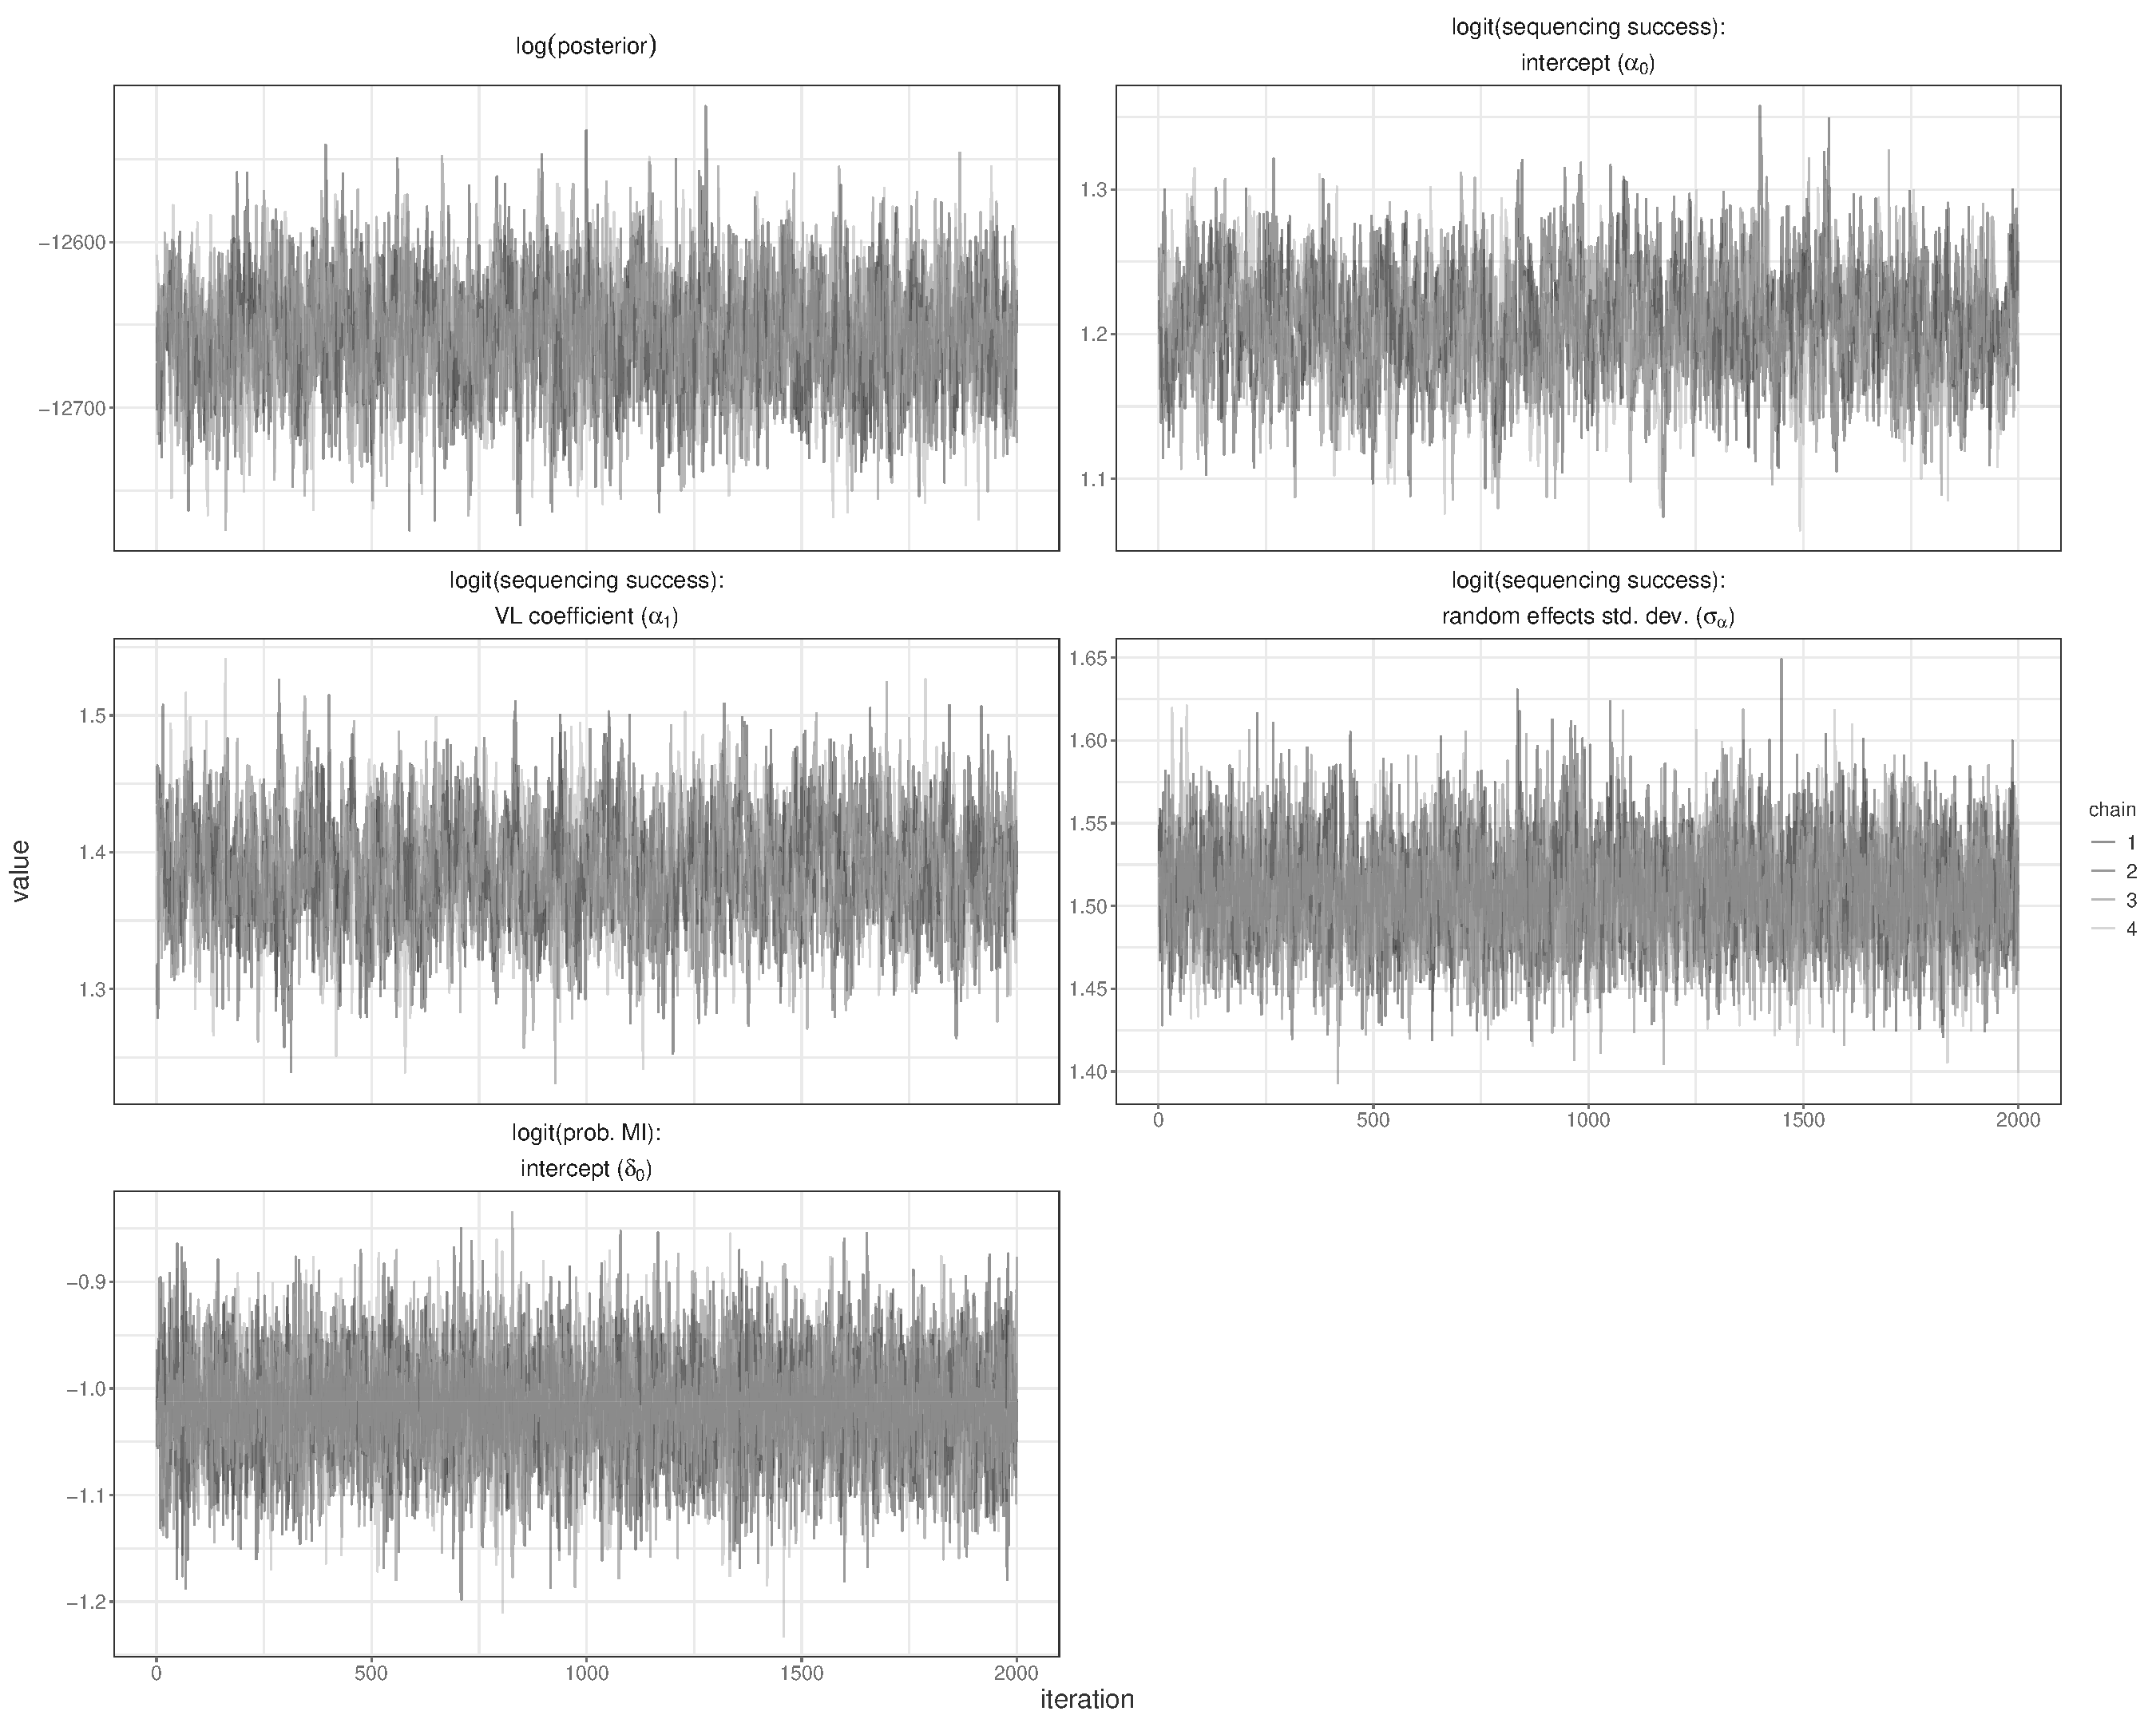
\includegraphics[width=1\textwidth]{../../figures/full_simulation_base_trace.pdf}}{}
\caption{{\bf MCMC trace plots for parameters in base model fit to simulated data with partial sequencing success and false positive and false negative multiple subgraph windows.} Independent chains are shown in shades of grey. Warm-up iterations are excluded. MI = multiple infection. VL = viral load (log\textsubscript{10} copies/mL) standardized to mean = 0 and std. dev = 1. Std. dev. = standard deviation.  }
\end{figure}

\begin{figure}[!ht]
 \ifthenelse{\boolean{includefigs}}{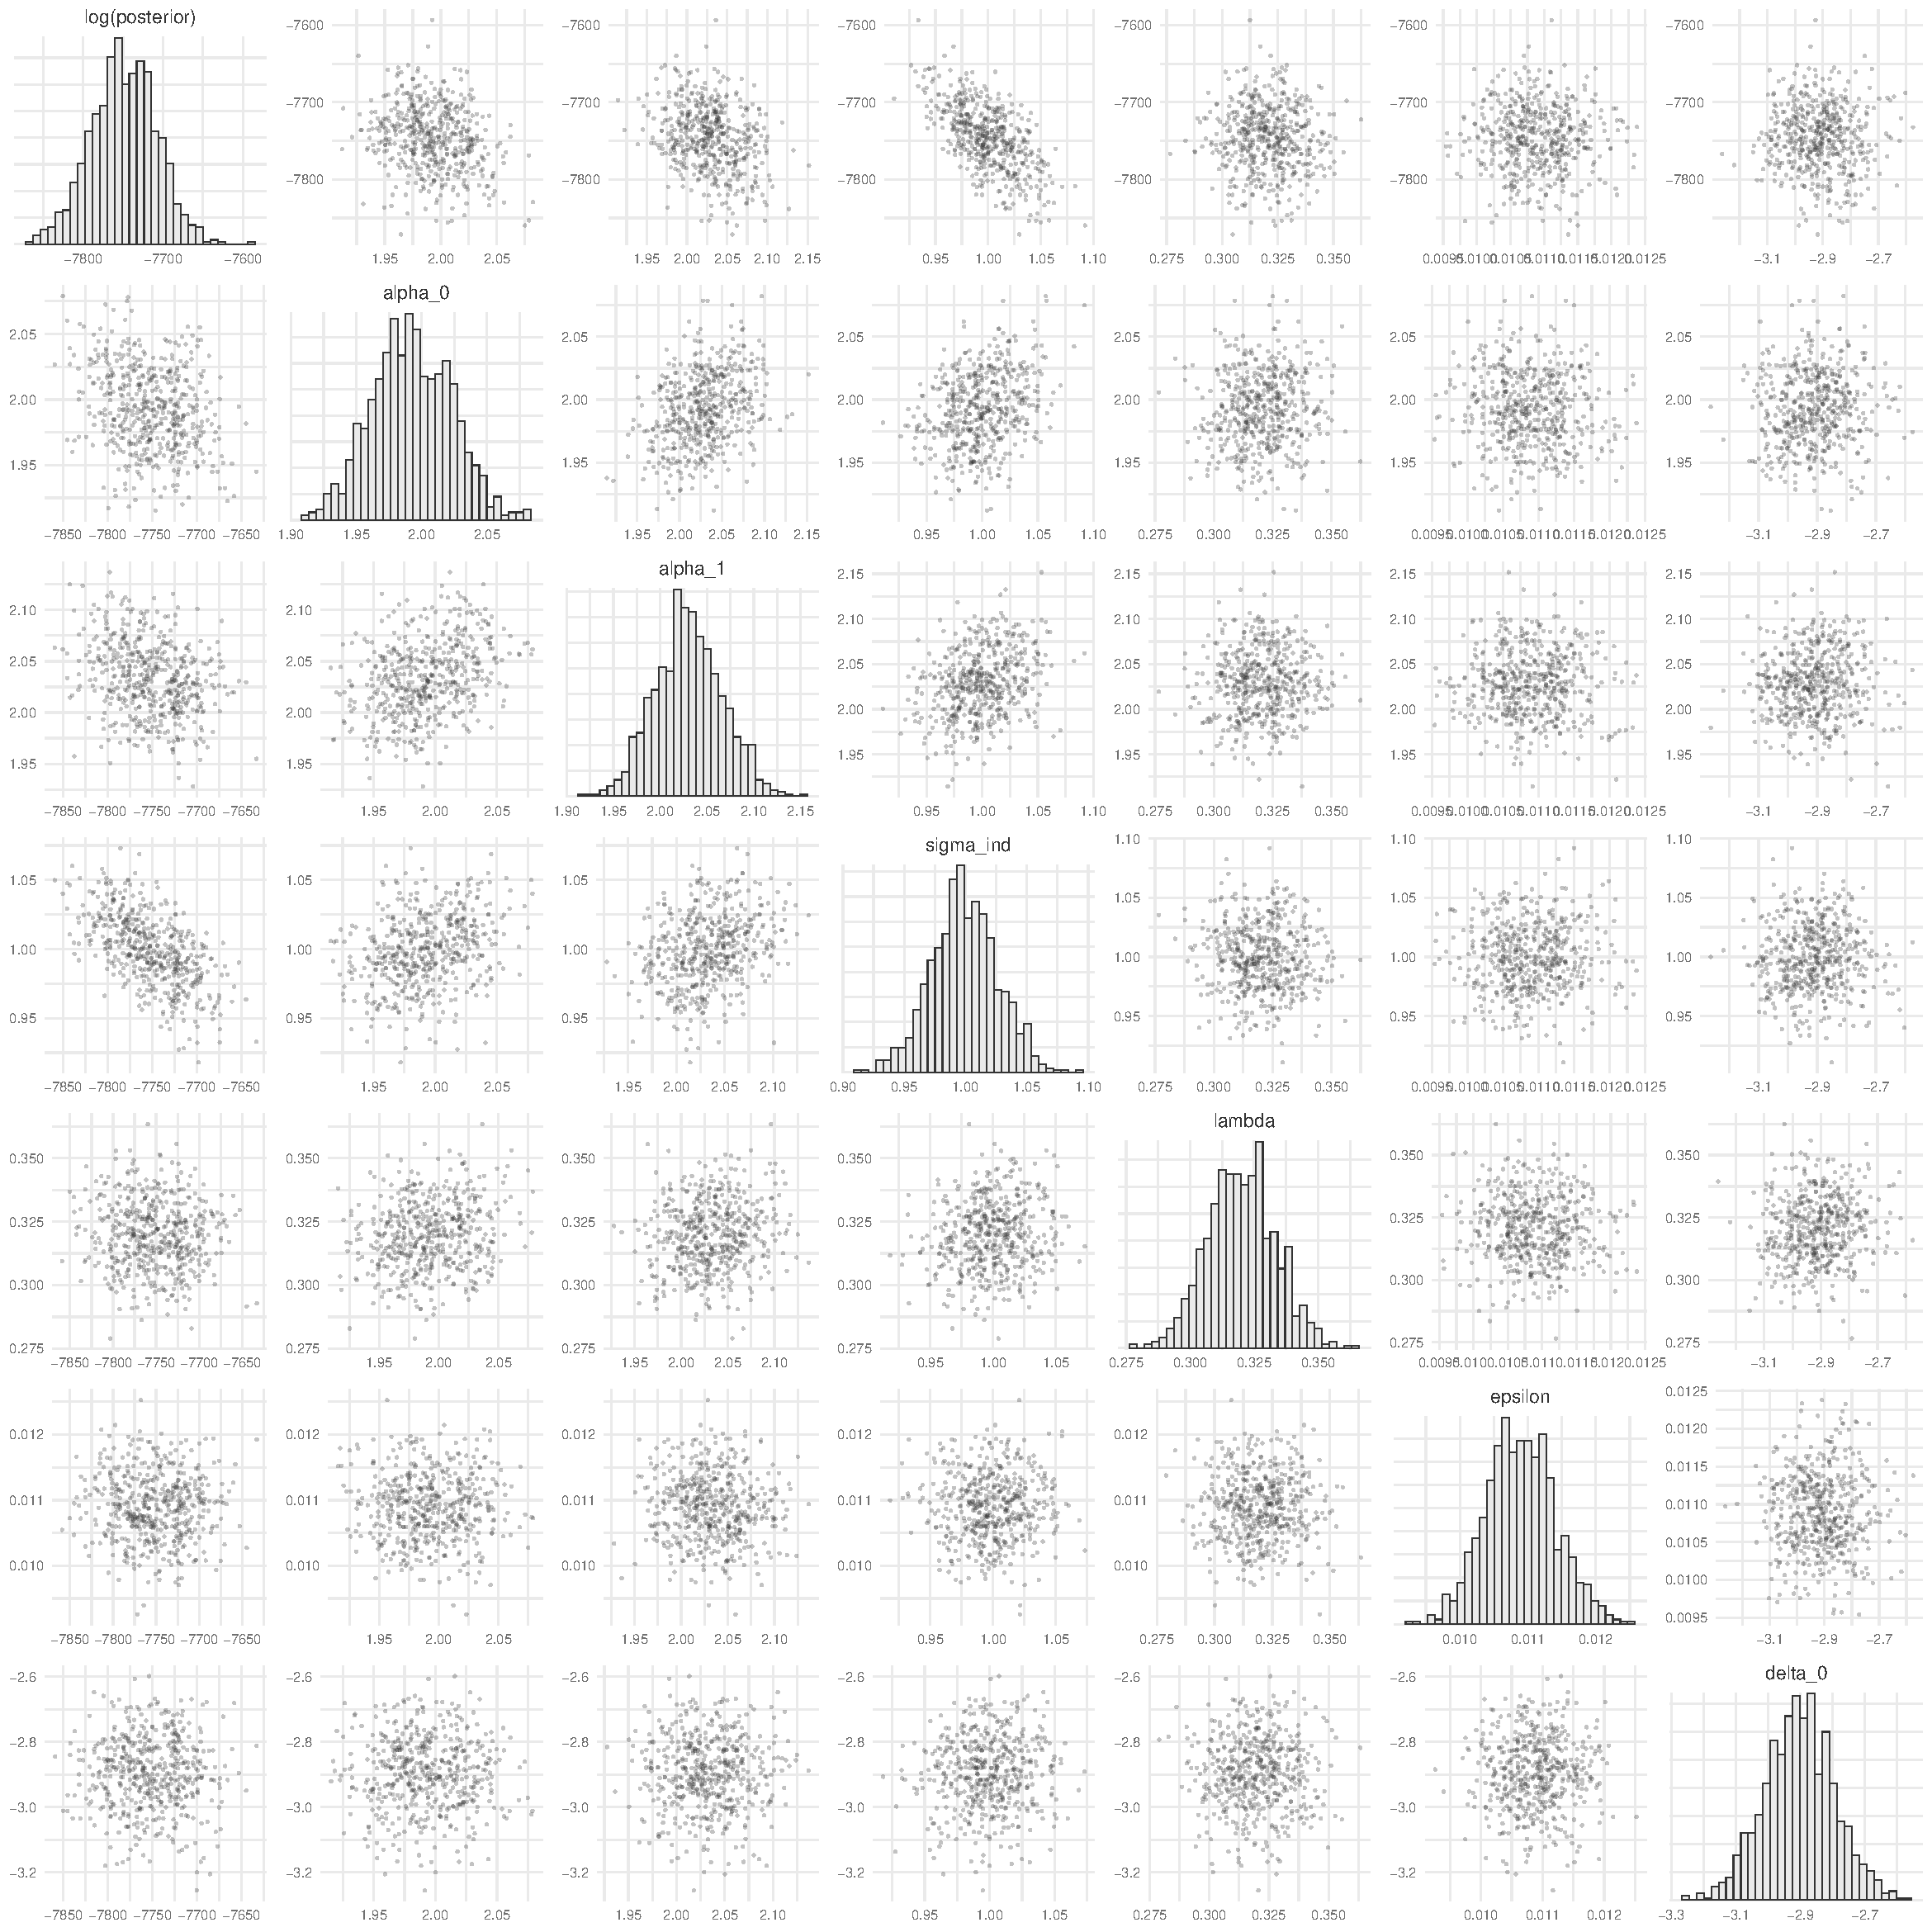
\includegraphics[width=1\textwidth]{../../figures/full_simulation_full_pairs.pdf}}{}
\caption{{\bf MCMC pairs plots for parameters in base model fit to simulated data with partial sequencing success and false positive and false negative multiple subgraph windows trace.} Independent chains are shown in shades of grey. Warm-up iterations are excluded. Includes a sample of 250 iterations per chain. MI = multiple infection.}
\end{figure}

\begin{figure}[!ht]
 \ifthenelse{\boolean{includefigs}}{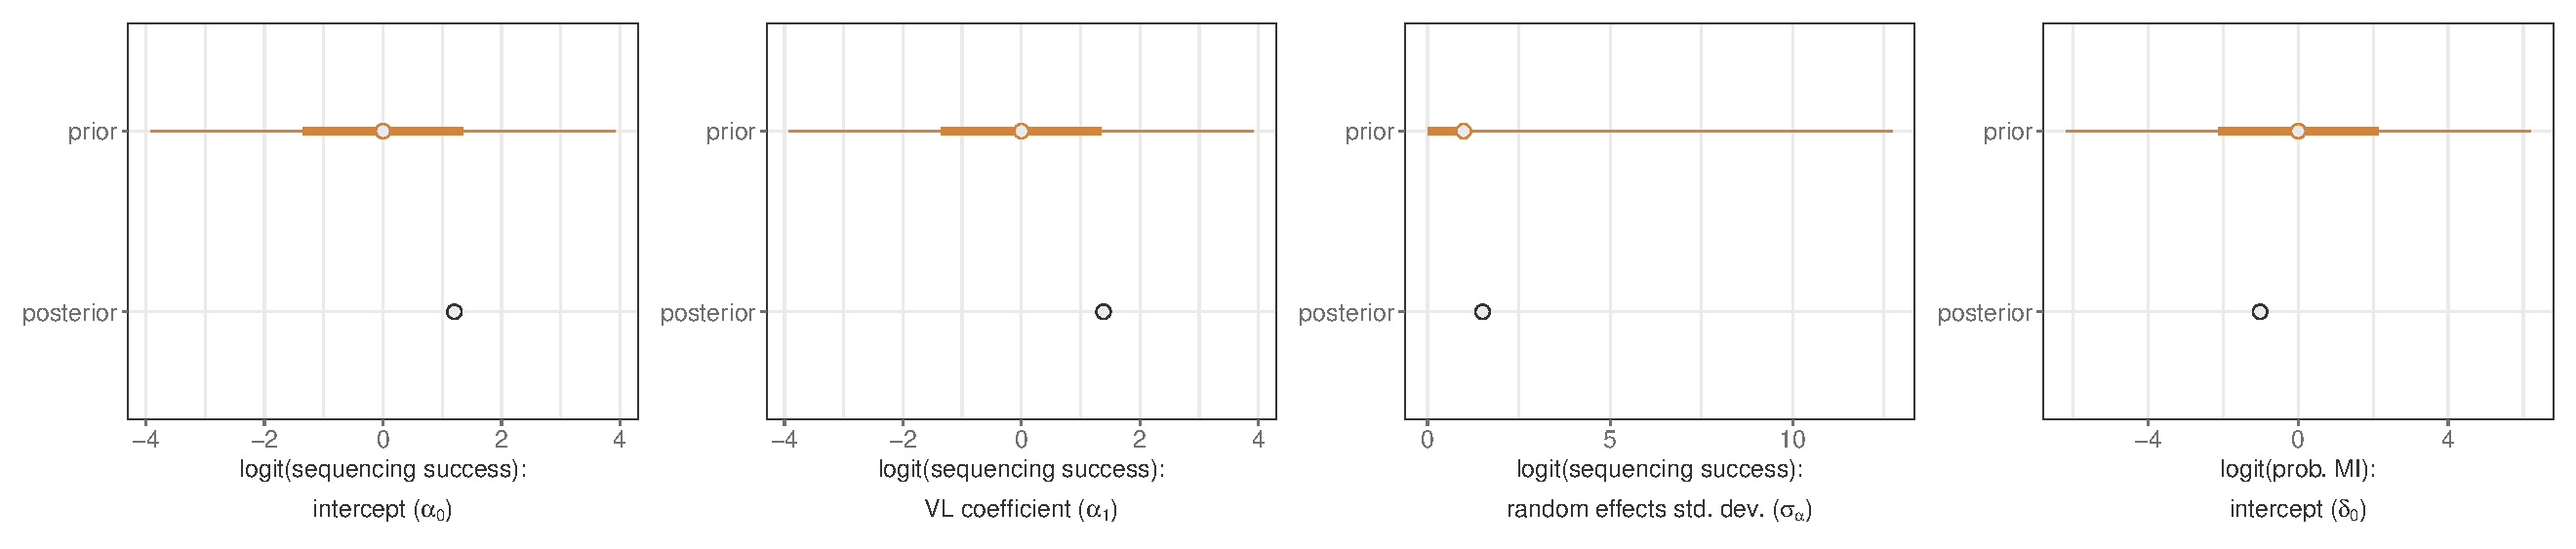
\includegraphics[width=1\textwidth]{../../figures/full_simulation_base_prior.pdf}}{}
\caption{{\bf Comparison of posterior and prior distributions of parameters in base model fit to simulated data with partial sequencing success and false positive or false negative multiple subgraph windows.} Median is plotted as the central estimate and horizontal bars extend to the 95\% and 50\% HPD. Some horizontal bars do not extend beyond the central point. Warm-up iterations are excluded. MI = multiple infection. VL = viral load (log\textsubscript{10} copies/mL) standardized to mean = 0 and std. dev = 1. Std. dev. = standard deviation. }
\end{figure}

\begin{figure}[!ht]
 \ifthenelse{\boolean{includefigs}}{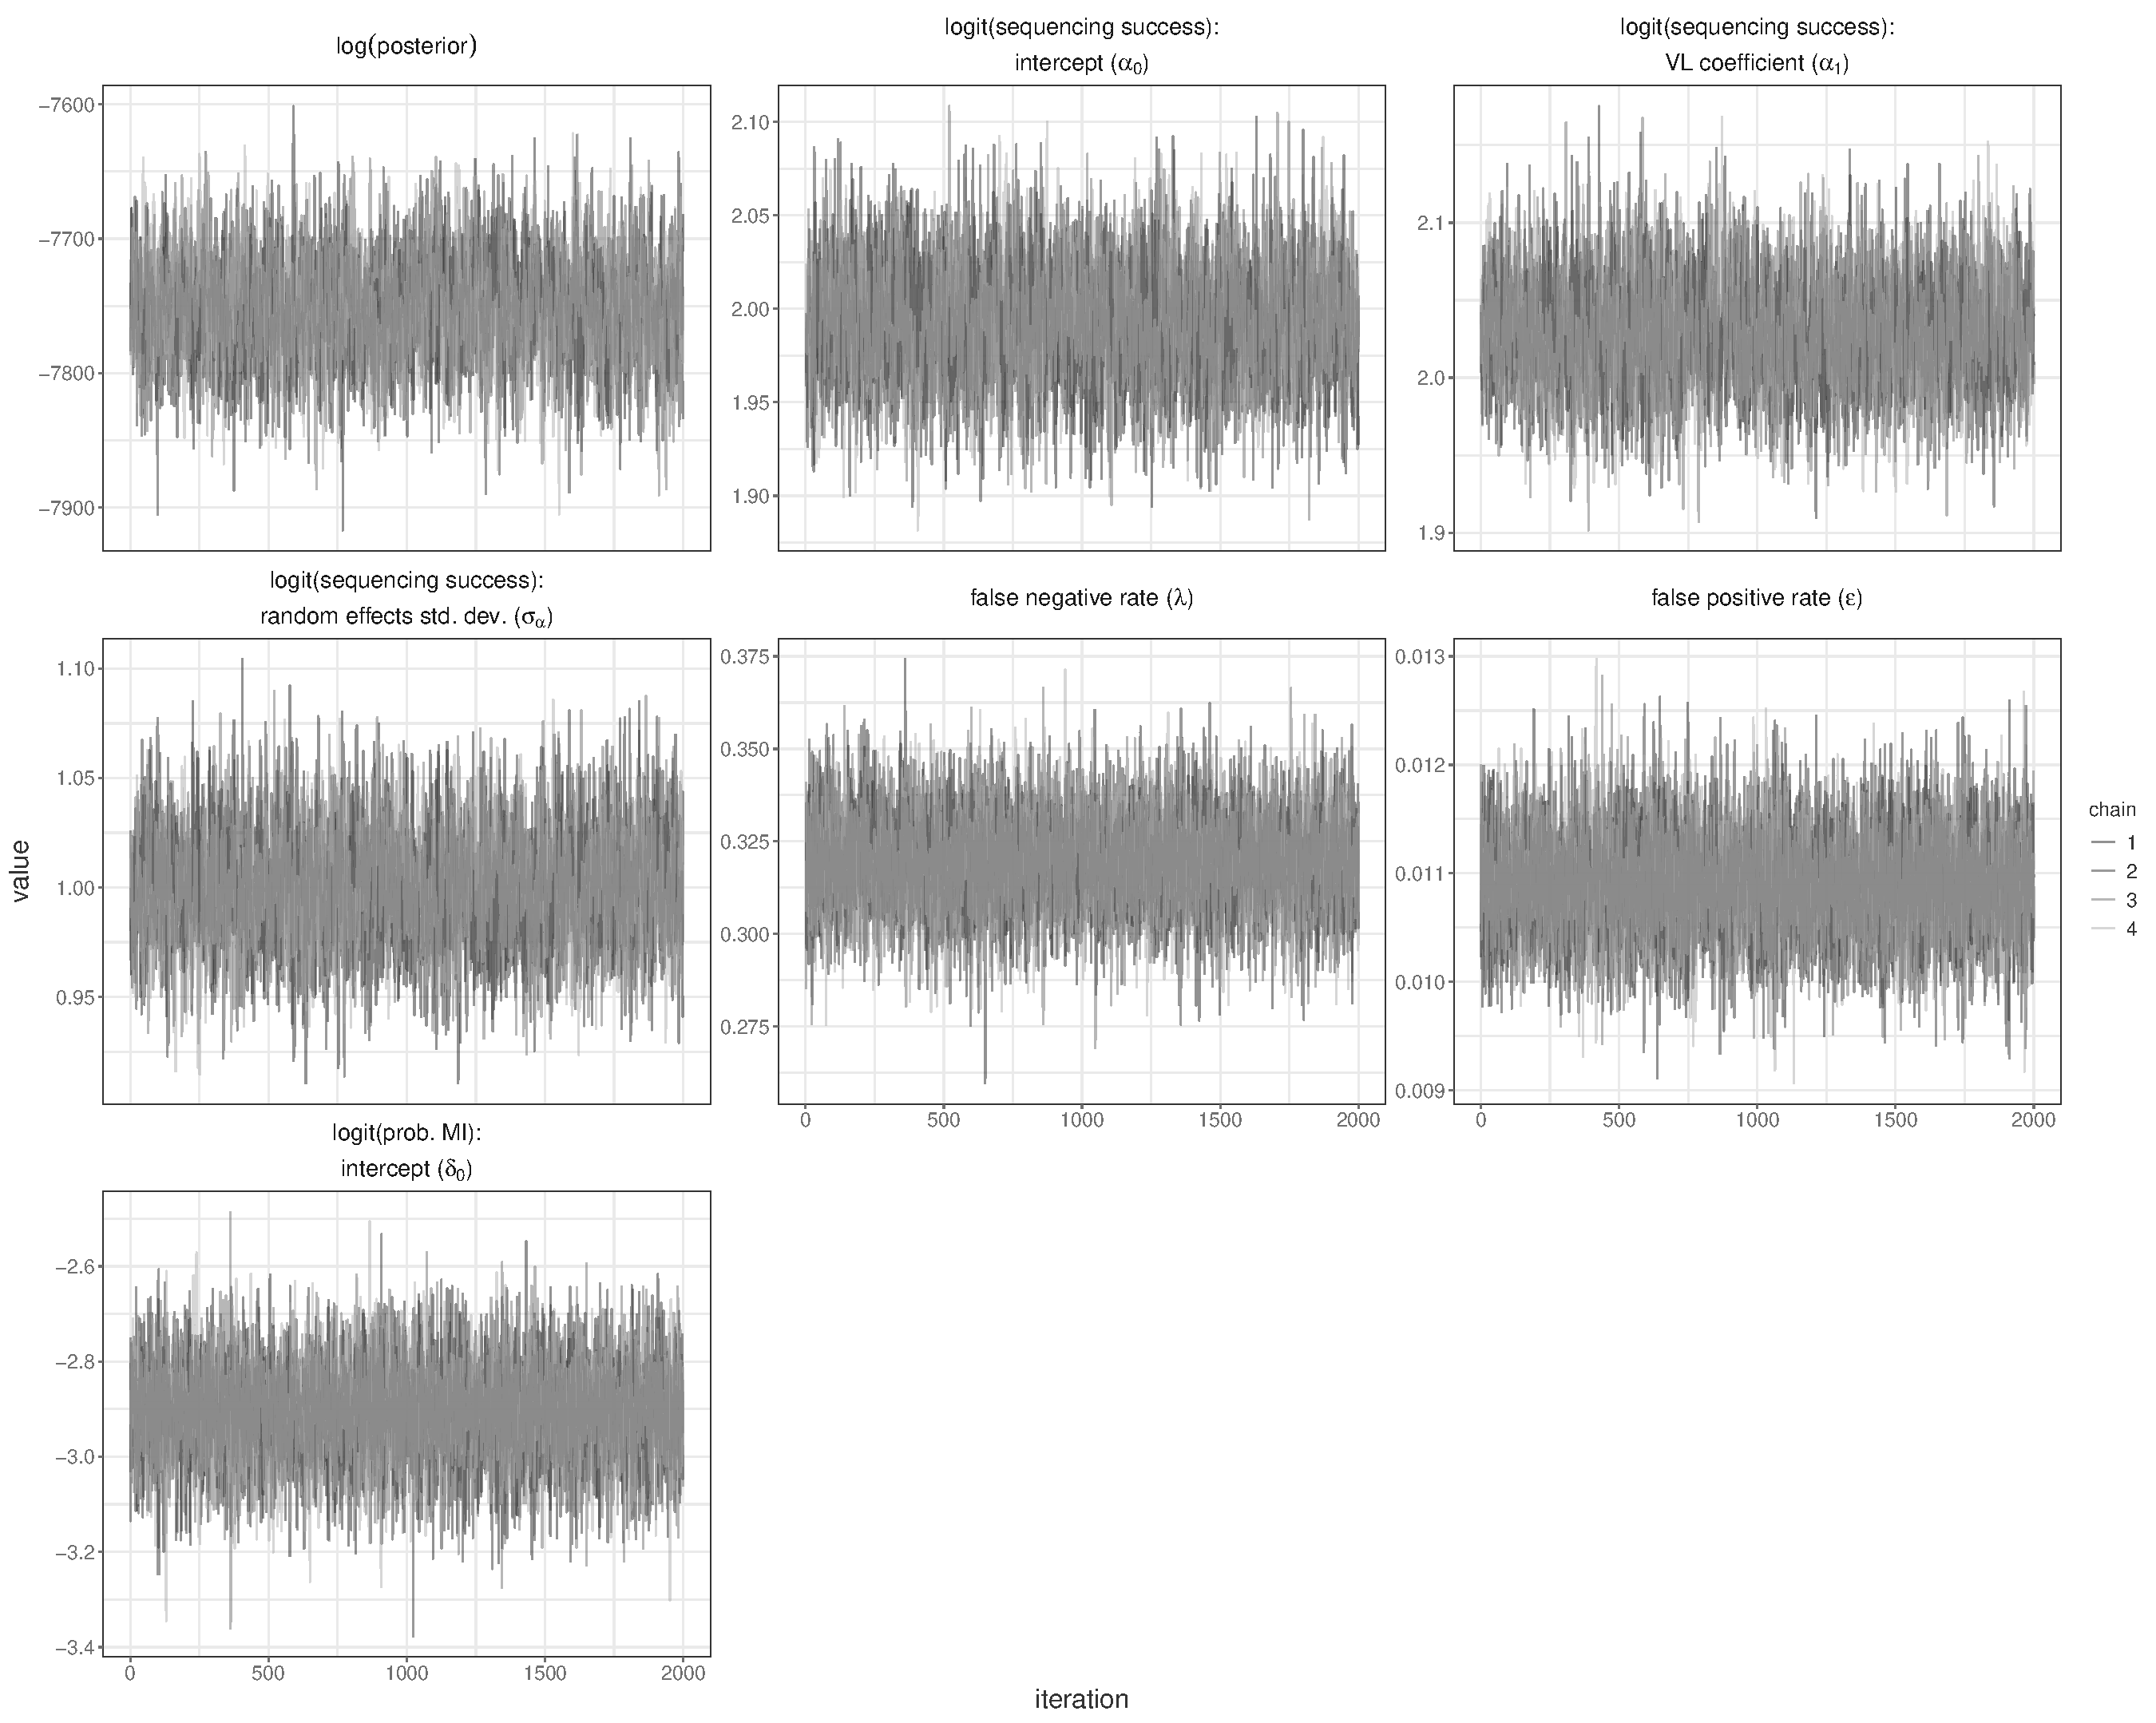
\includegraphics[width=1\textwidth]{../../figures/full_simulation_full_trace.pdf}}{}
\caption{{\bf MCMC trace plots for parameters in full model fit to simulated data with partial sequencing success and false positive and false negative multiple subgraph windows.} Independent chains are shown in shades of grey. Warm-up iterations are excluded.MI = multiple infection. VL = viral load (log\textsubscript{10} copies/mL) standardized to mean = 0 and std. dev = 1. Std. dev. = standard deviation. }
\end{figure}

\begin{figure}[!ht]
 \ifthenelse{\boolean{includefigs}}{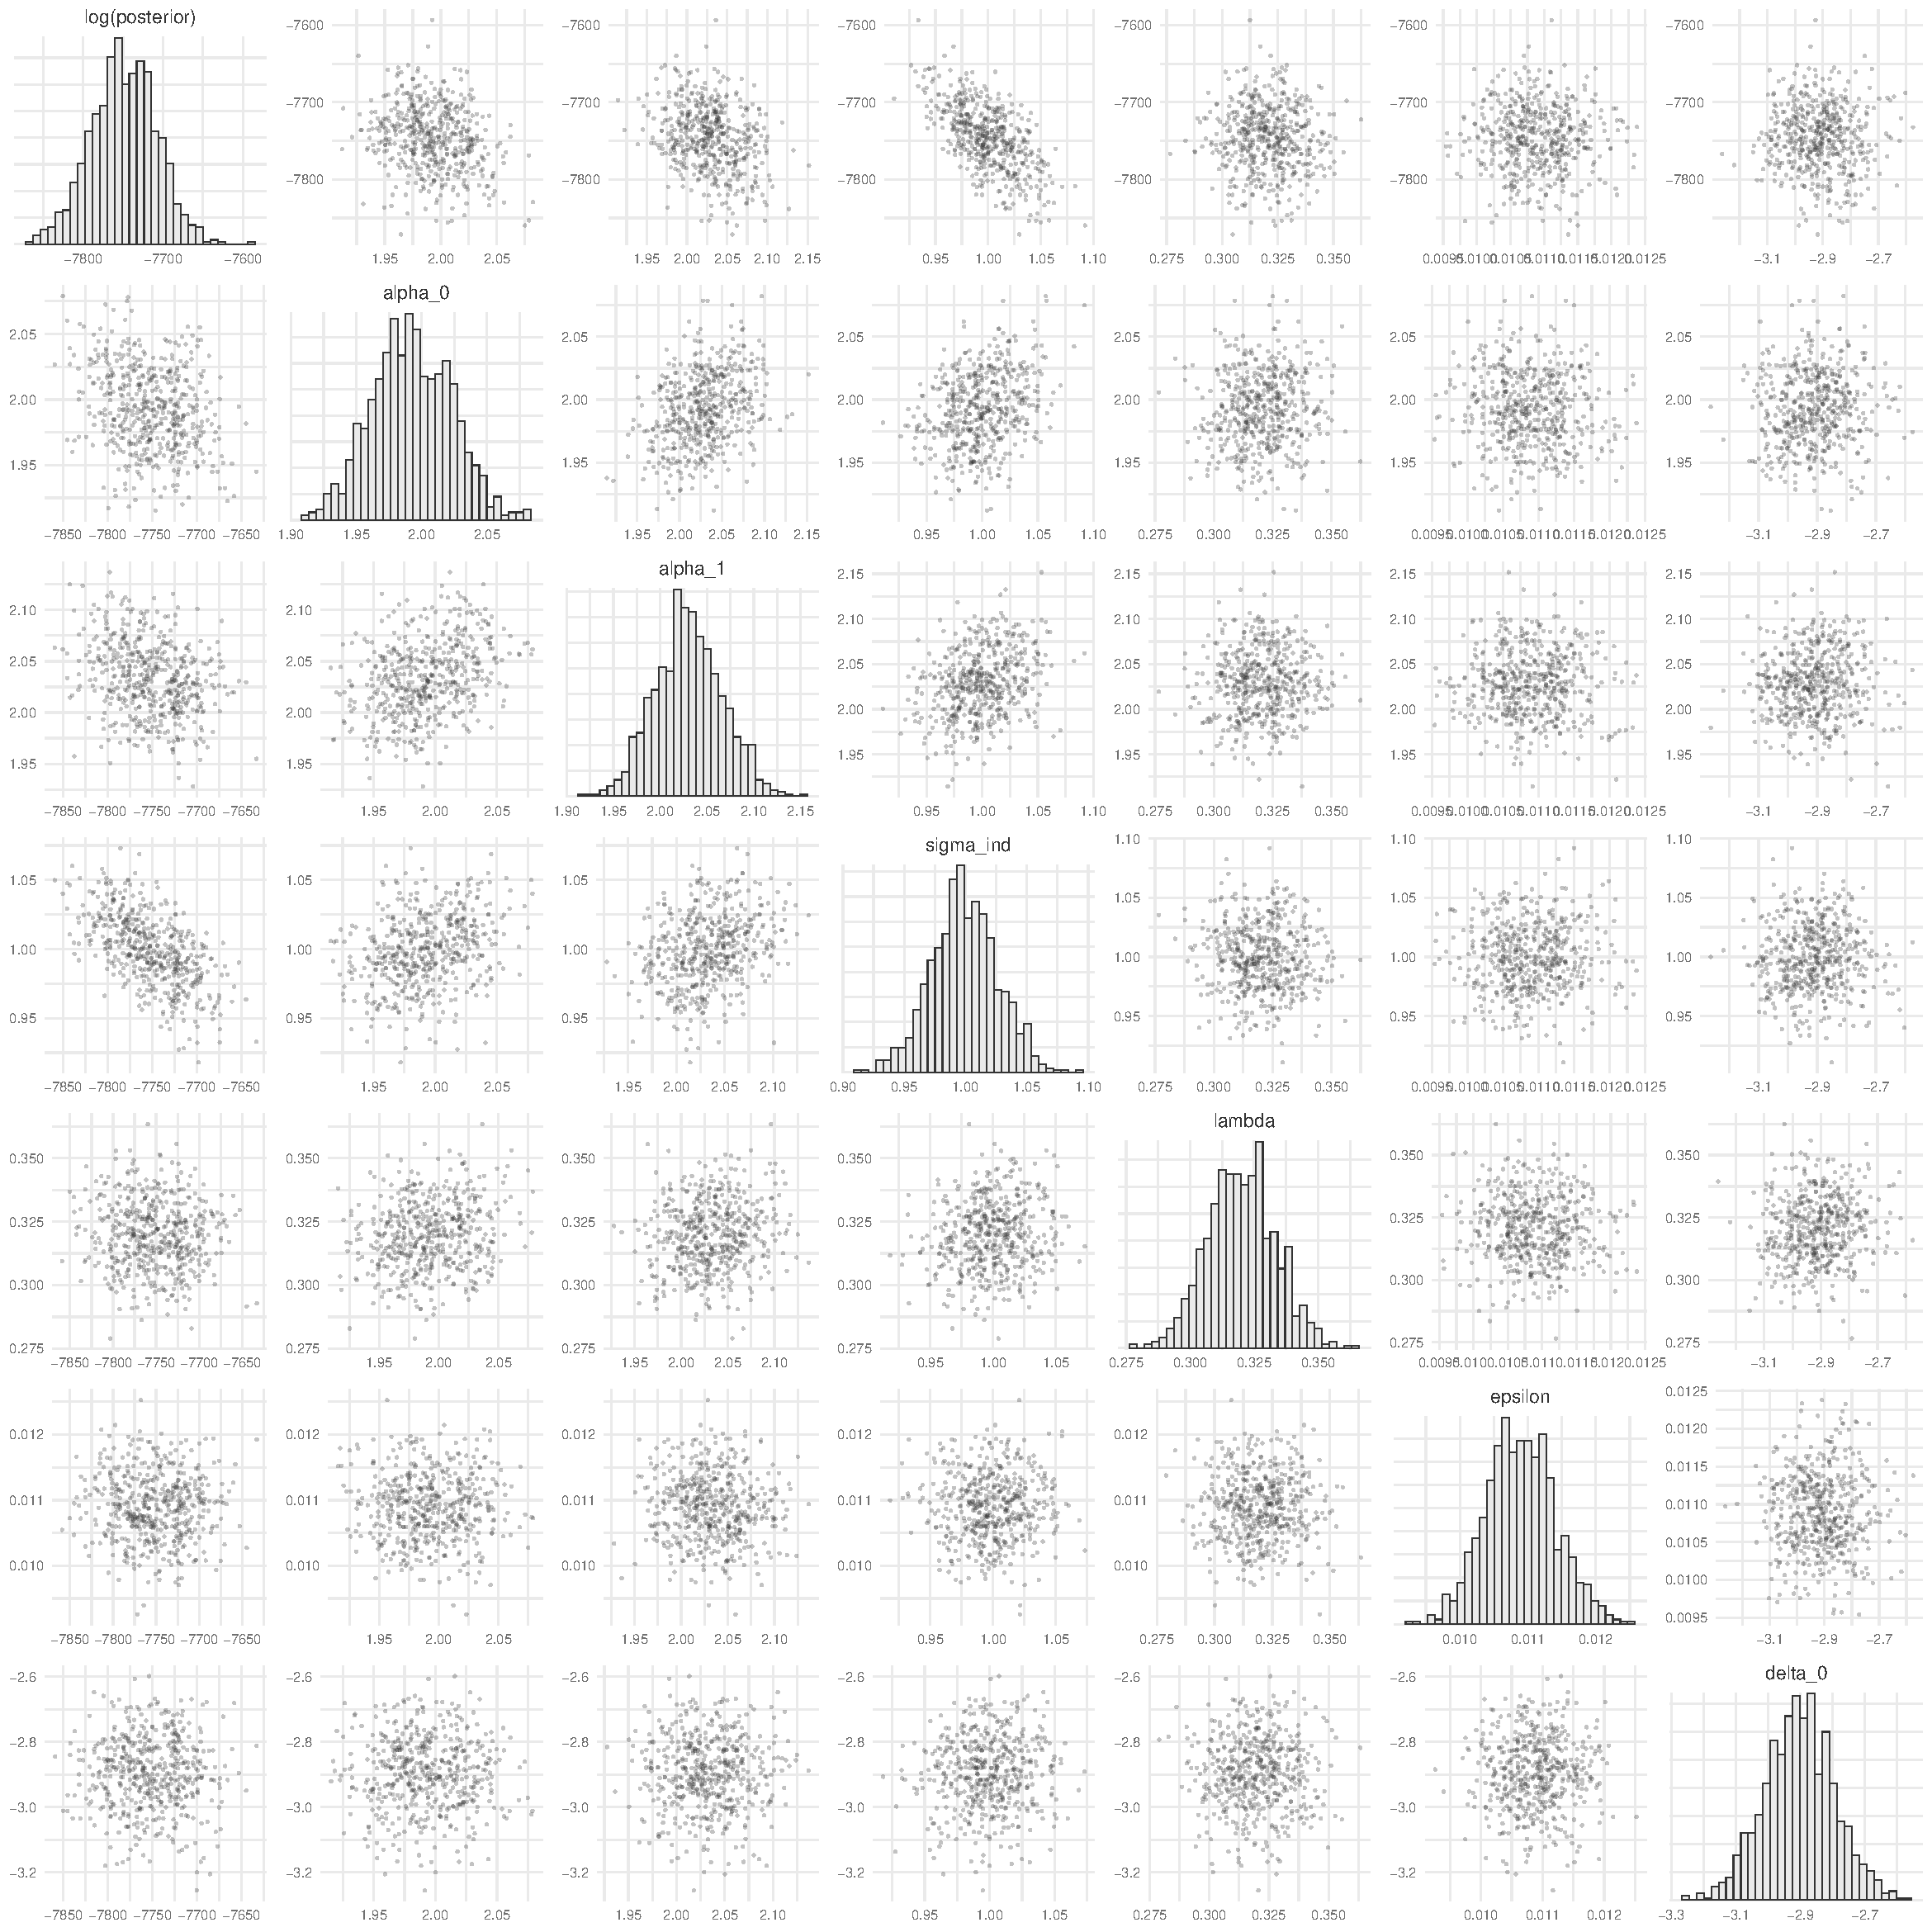
\includegraphics[width=1\textwidth]{../../figures/full_simulation_full_pairs.pdf}}{}
\caption{{\bf MCMC pairs plots for parameters in full model fit to simulated data with partial sequencing success and false positive and false negative multiple subgraph windows trace.} Independent chains are shown in shades of grey. Warm-up iterations are excluded. MI = multiple infection.  }
\end{figure}

\begin{figure}[!ht]
 \ifthenelse{\boolean{includefigs}}{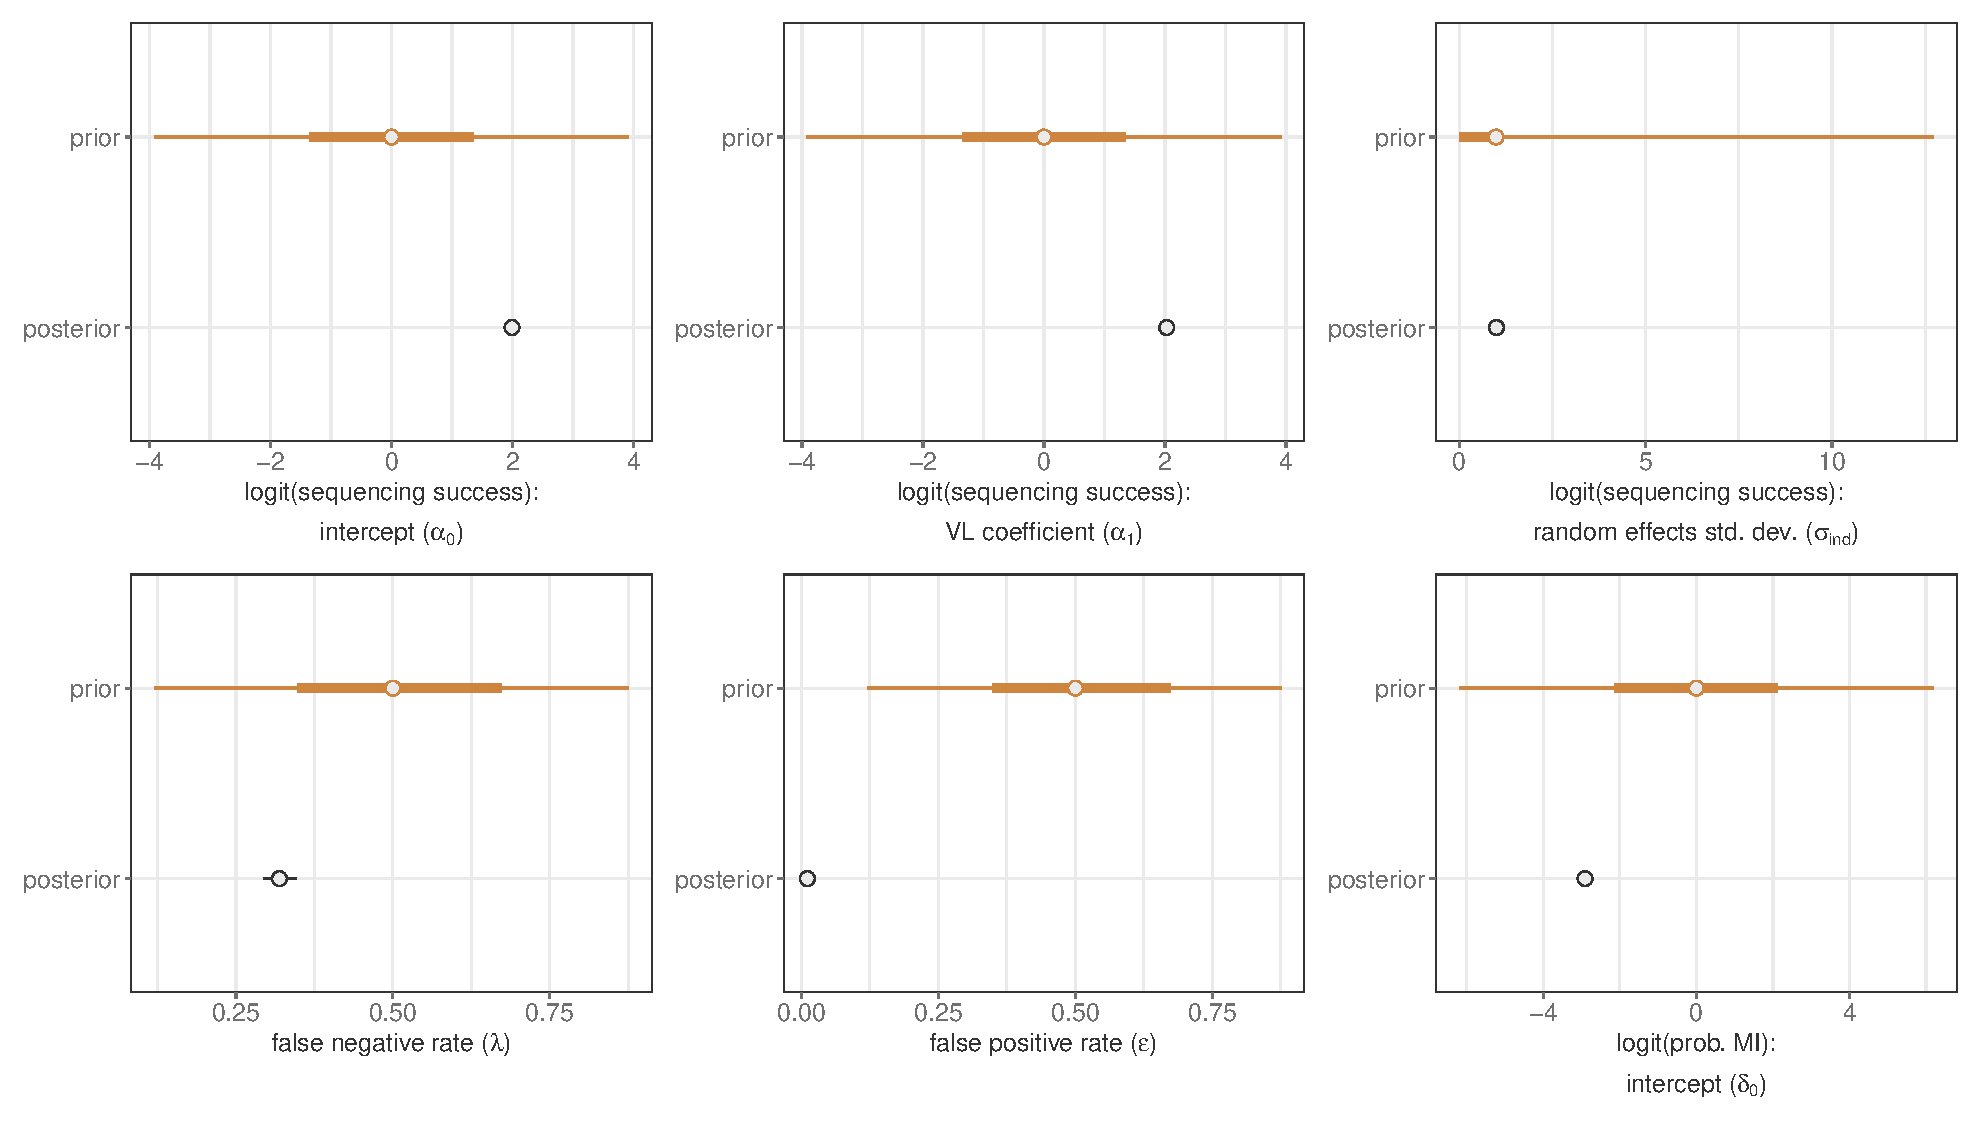
\includegraphics[width=1\textwidth]{../../figures/full_simulation_full_prior.pdf}}{}
\caption{{\bf Comparison of posterior and prior distributions of parameters in full model fit to simulated data with partial sequencing success and false positive or false negative multiple subgraph windows.} Median is plotted as the central estimate and horizontal bars extend to the 95\% and 50\% HPD. Some horizontal bars do not extend beyond the central point. Warm-up iterations are excluded. MI = multiple infection. VL = viral load (log\textsubscript{10} copies/mL) standardized to mean = 0 and std. dev = 1. Std. dev. = standard deviation. }
\end{figure}

% extended simulation
\begin{figure}[!ht]
 \ifthenelse{\boolean{includefigs}}{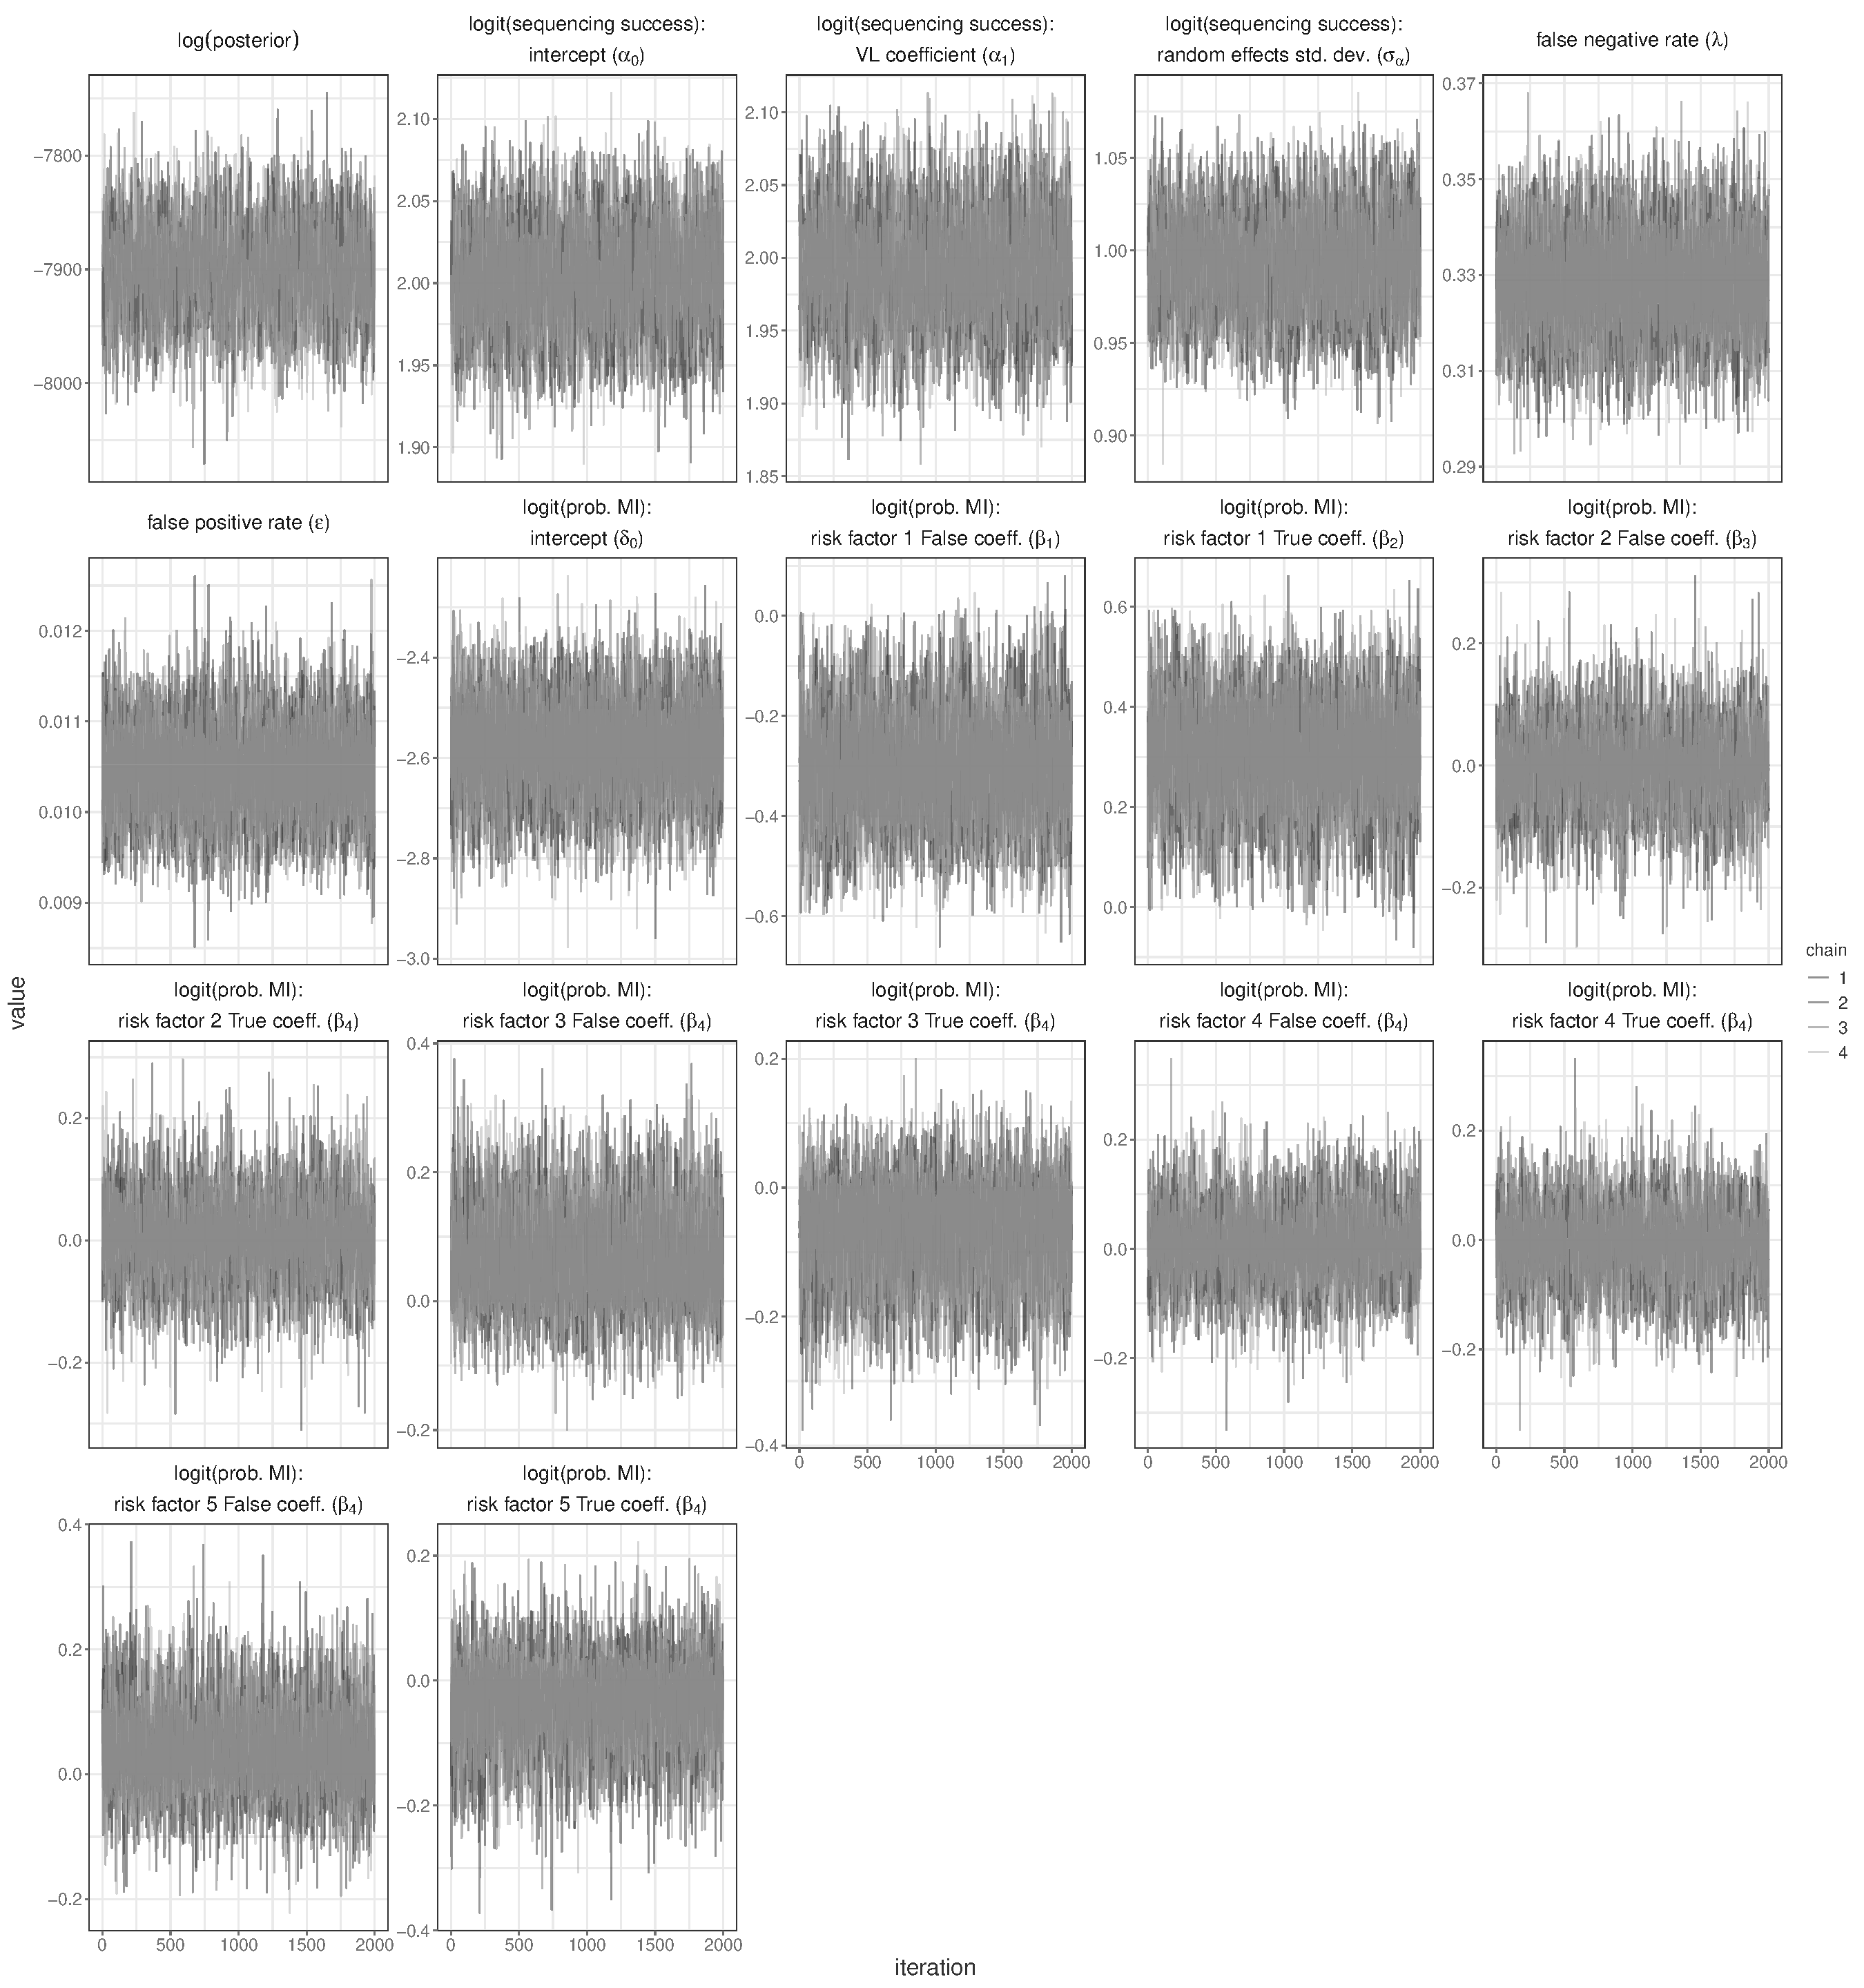
\includegraphics[width=1\textwidth]{../../figures/extended_simulation_extended_trace.pdf}}{}
\caption{{\bf MCMC trace plots for parameters in extended model fit to simulated data with partial sequencing success, false positive and false negative multiple subgraph windows, and a binary risk factor for harboring multiple infection.} Independent chains are shown in shades of grey. Warm-up iterations are excluded. MI = multiple infection. VL = viral load (log\textsubscript{10} copies/mL) standardized to mean = 0 and std. dev = 1. Std. dev. = standard deviation.  }
\end{figure}

\begin{figure}[!ht]
 \ifthenelse{\boolean{includefigs}}{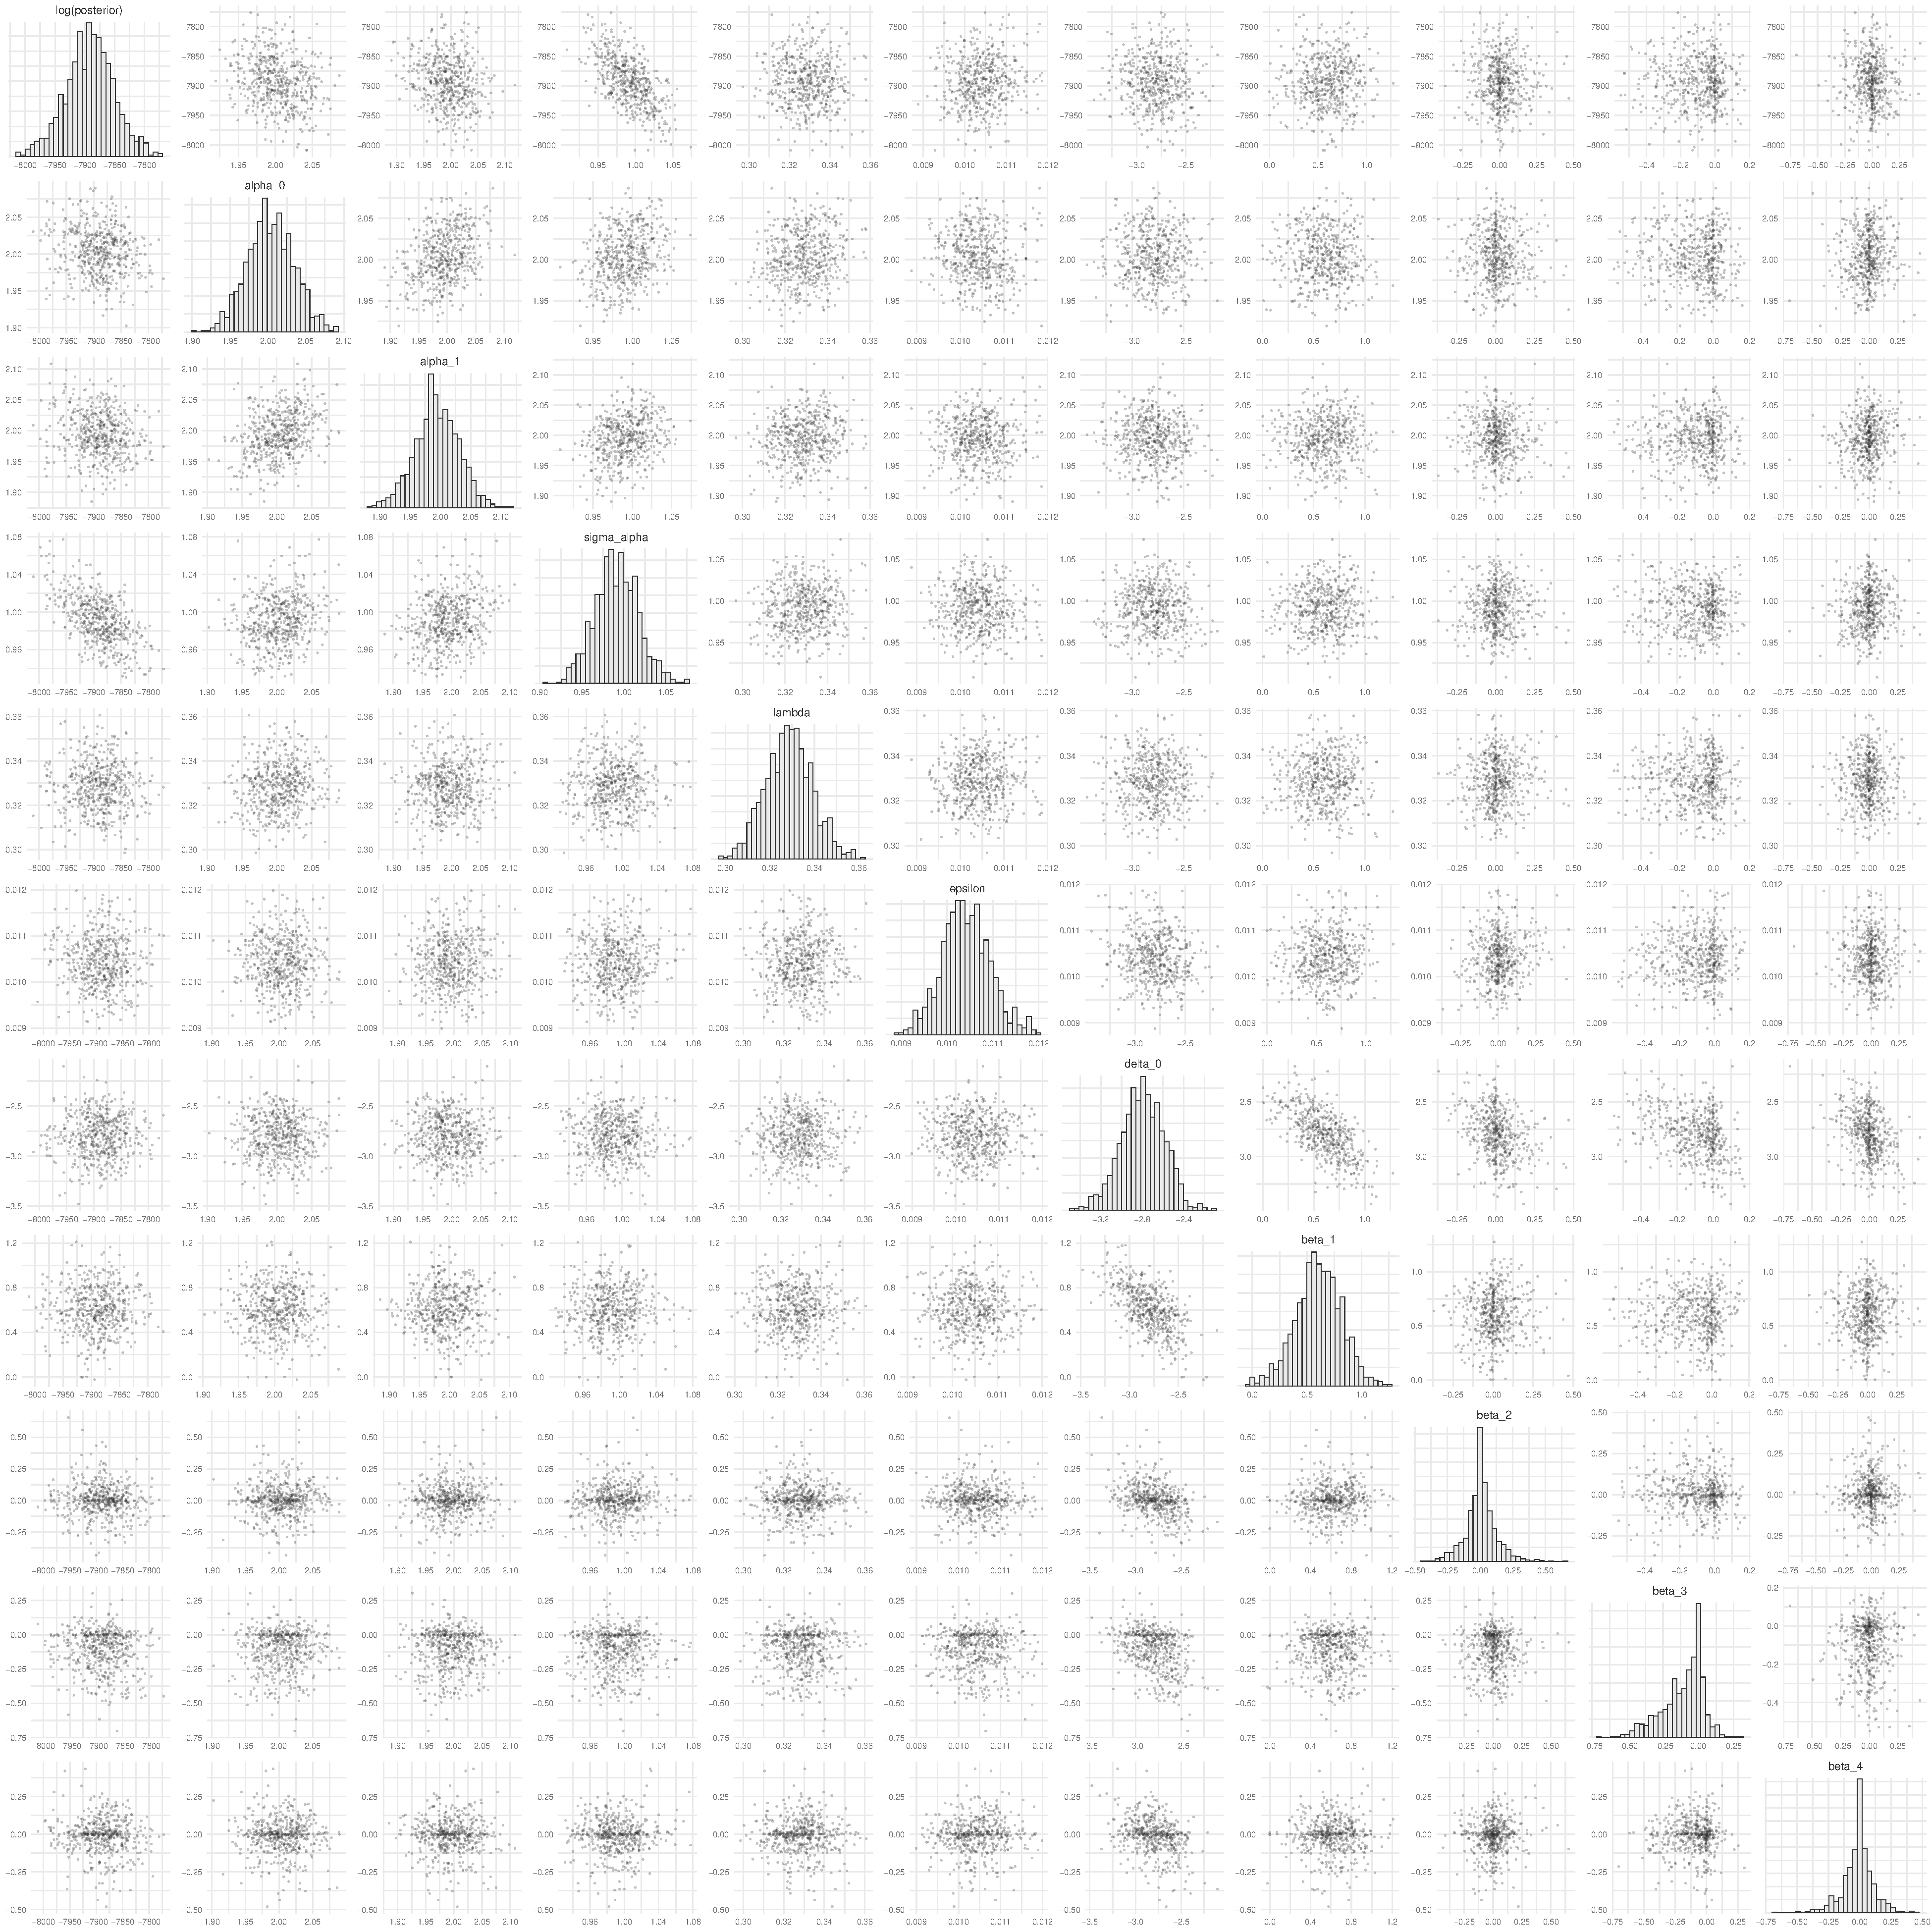
\includegraphics[width=1\textwidth]{../../figures/extended_simulation_extended_pairs.pdf}}{}
\caption{{\bf MCMC pairs plots for parameters in  extended model fit to simulated data with partial sequencing success, false positive and false negative multiple subgraph windows, and a binary risk factor for harboring multiple infection.} Independent chains are shown in shades of grey. Warm-up iterations are excluded. Includes a sample of 250 iterations per chain. MI = multiple infection. }
\end{figure}

\begin{figure}[!ht]
 \ifthenelse{\boolean{includefigs}}{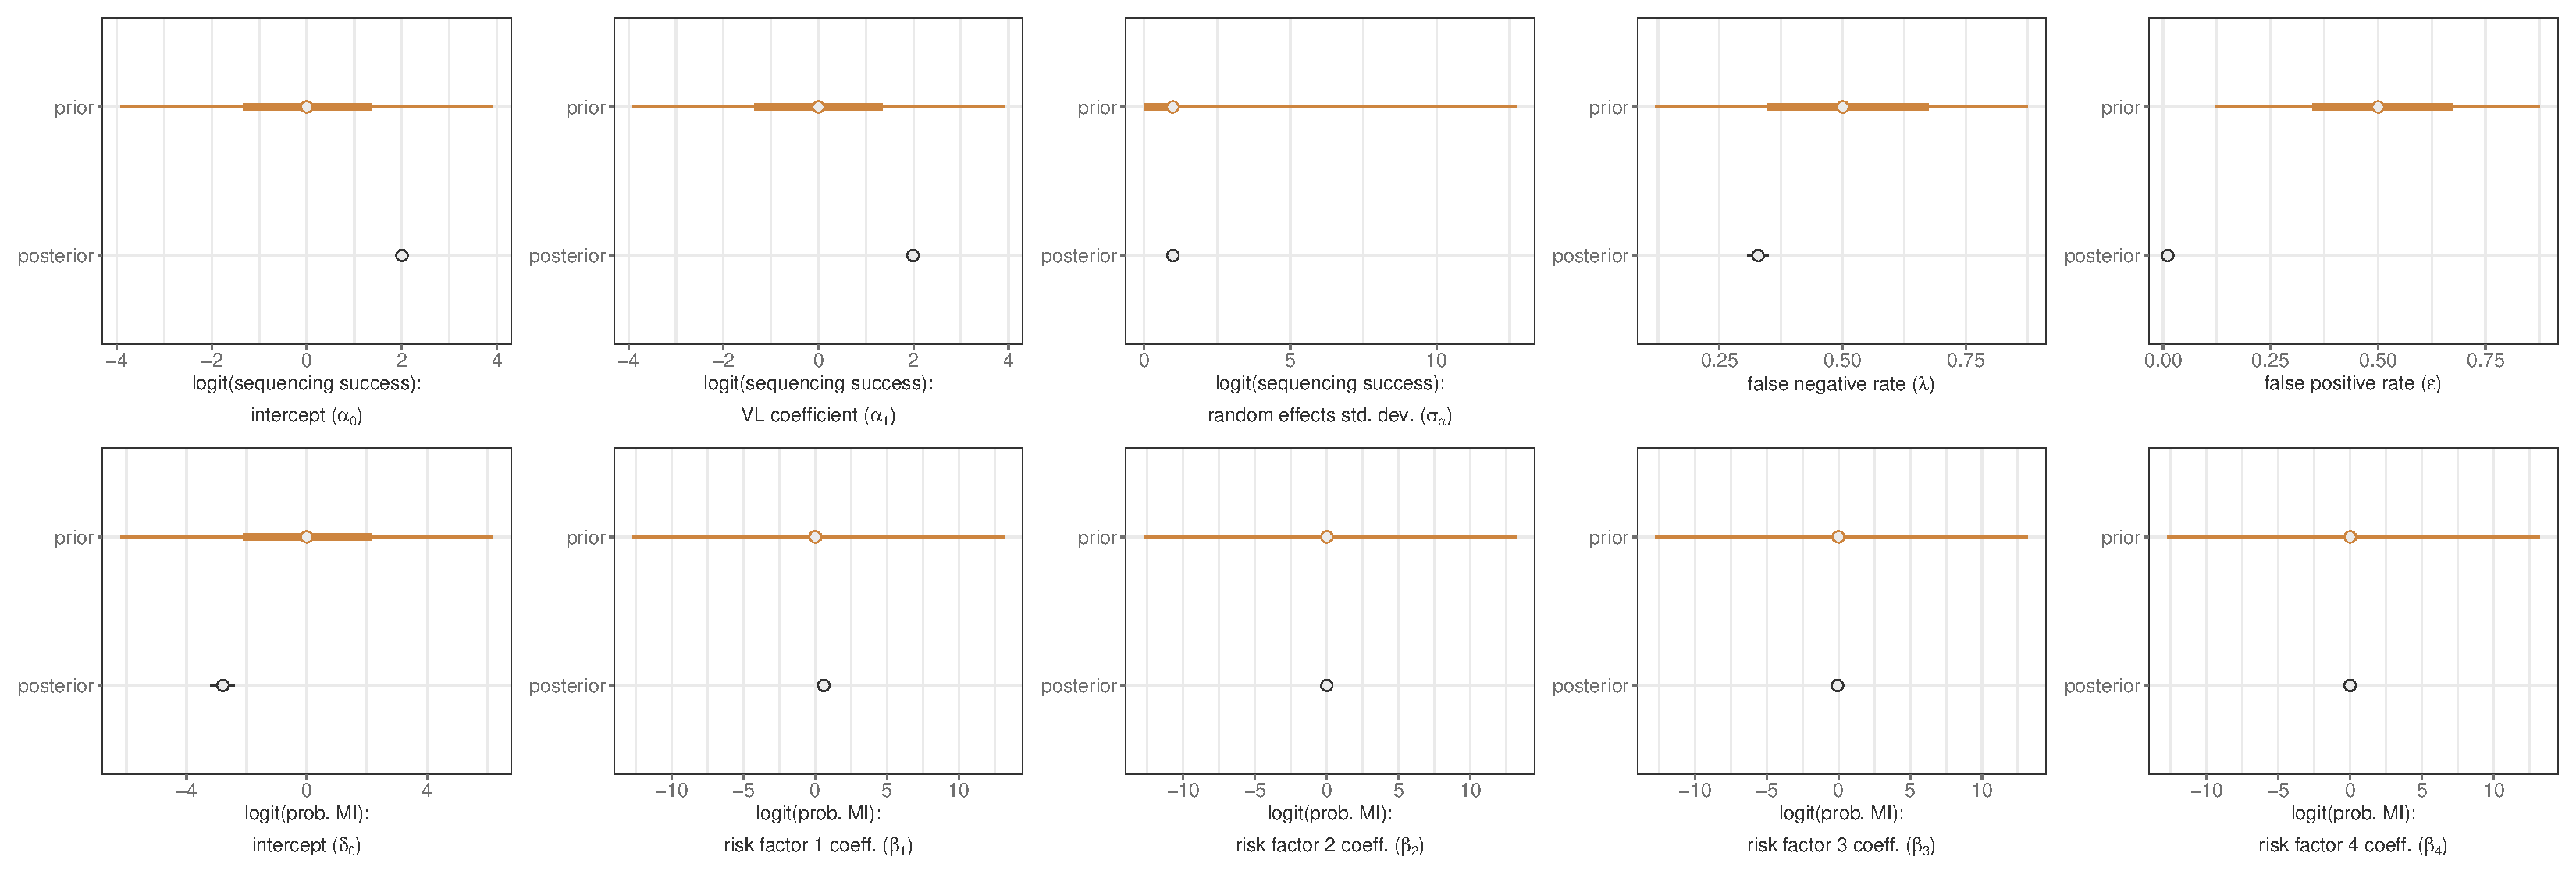
\includegraphics[width=1\textwidth]{../../figures/extended_simulation_extended_prior.pdf}}{}
\caption{{\bf Comparison of posterior and prior distributions of parameters in full model fit to simulated data with partial sequencing success, false positive or false negative multiple subgraph windows, and a binary risk factor for harboring multiple infection.} Median is plotted as the central estimate and horizontal bars extend to the 95\% and 50\% HPD. Some horizontal bars do not extend beyond the central point. Warm-up iterations are excluded. MI = multiple infection. VL = viral load (log\textsubscript{10} copies/mL) standardized to mean = 0 and std. dev = 1. Std. dev. = standard deviation. }
\end{figure}

% empirical full
\begin{figure}[!ht]
 \ifthenelse{\boolean{includefigs}}{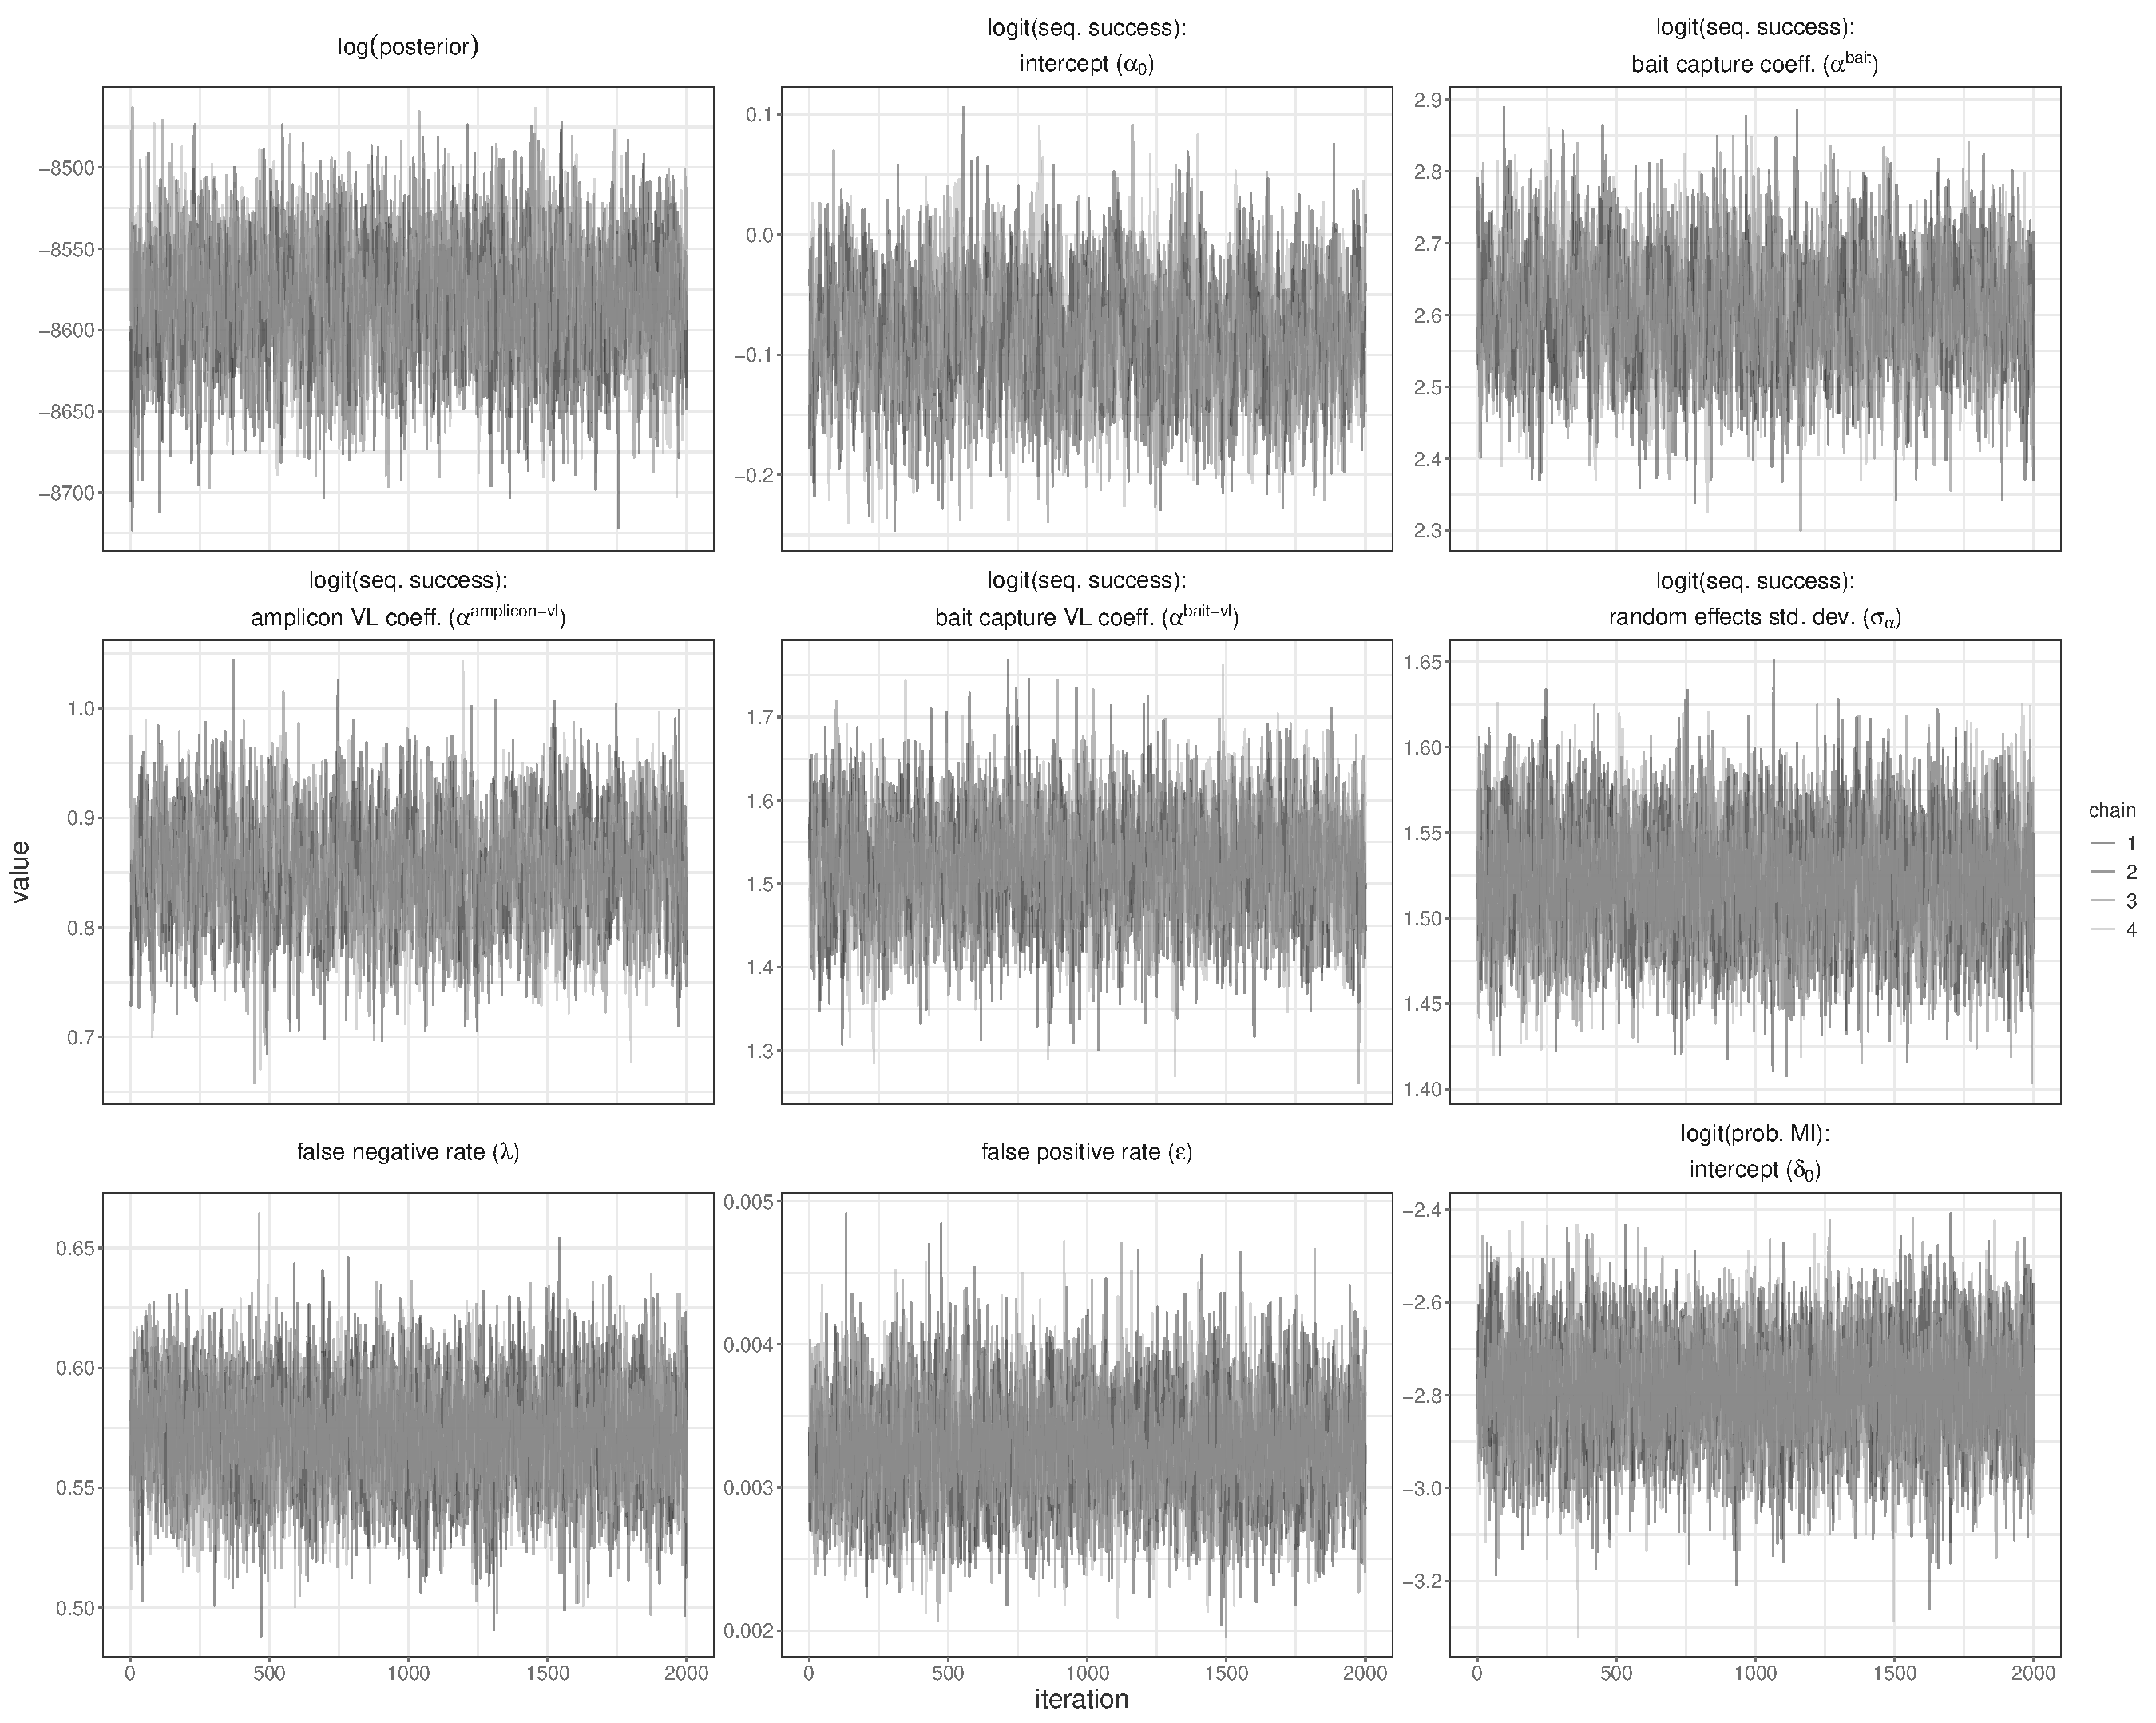
\includegraphics[width=1\textwidth]{../../figures/empirical_full_trace.pdf}}{}
\caption{{\bf MCMC trace plots for parameters in full model fit to deep sequence data generated from \protect \var{empirical_full_n_participant_visits} Rakai Community Cohort Study participants living with viremic HIV.} Independent chains are shown in shades of grey. Warm-up iterations are excluded. MI = multiple infection. VL = viral load (log\textsubscript{10} copies/mL) standardized to mean = 0 and std. dev = 1. Std. dev. = standard deviation. }
\end{figure}

\begin{figure}[!ht]
 \ifthenelse{\boolean{includefigs}}{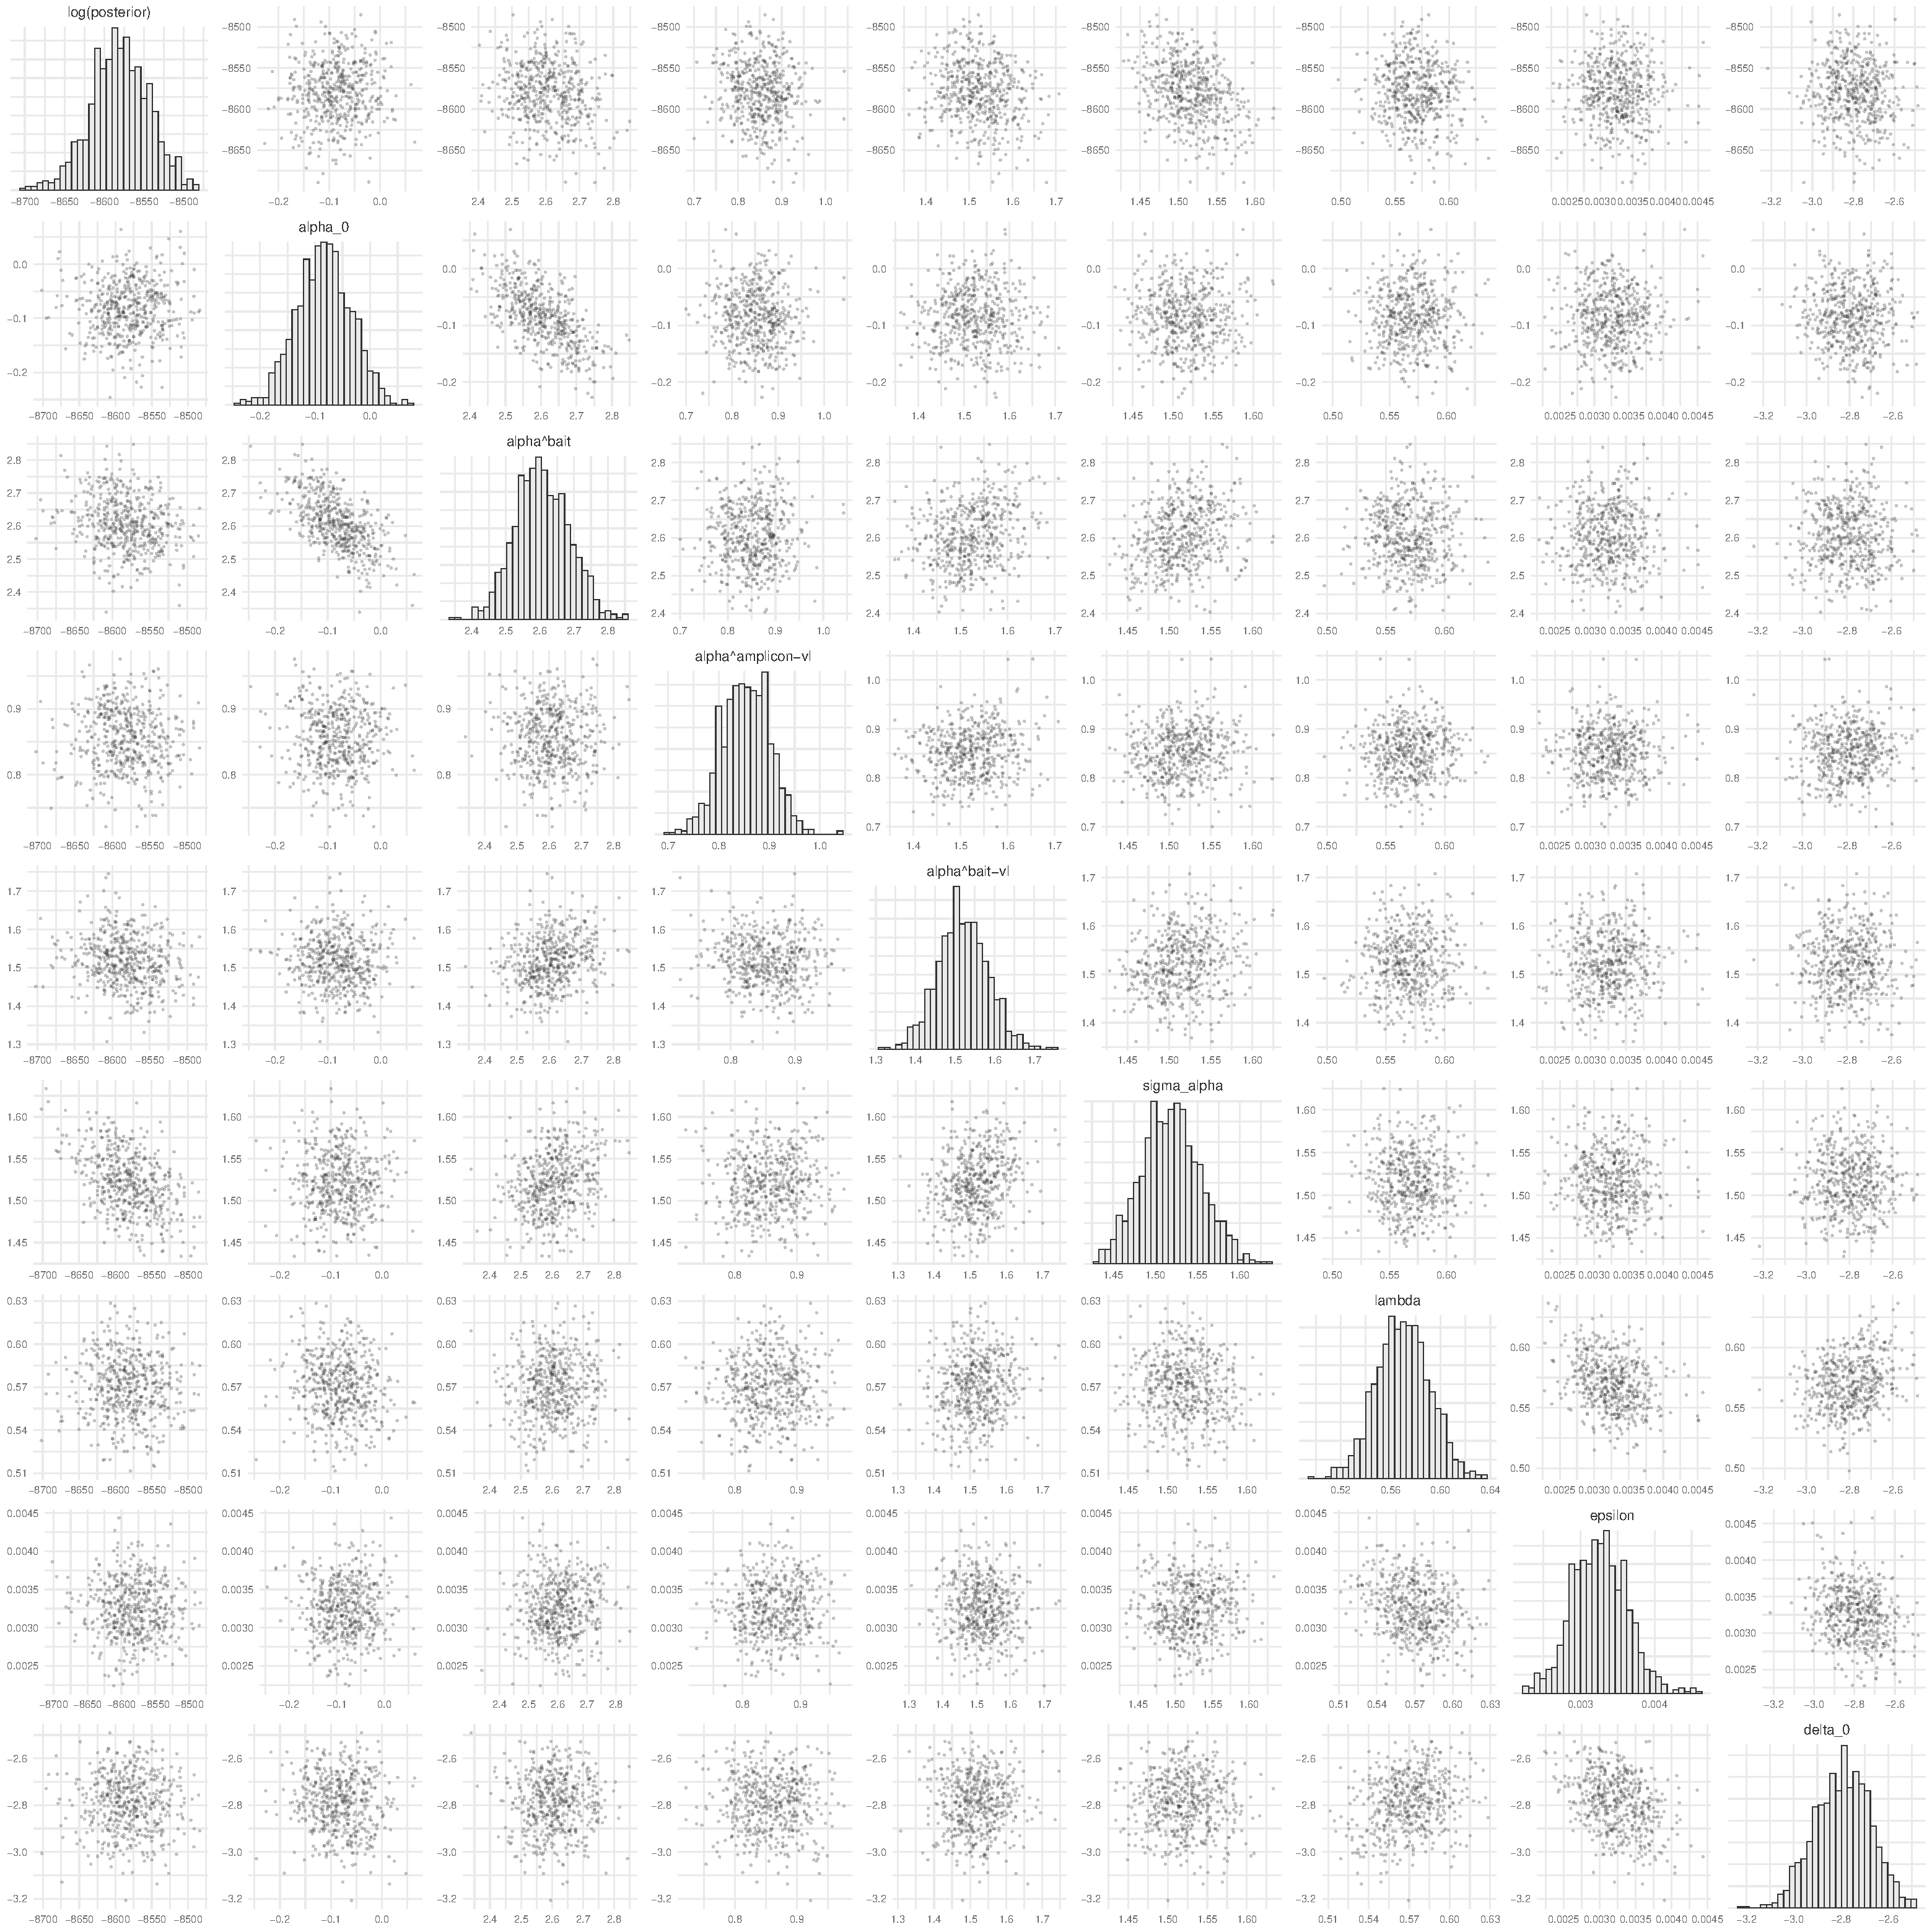
\includegraphics[width=1\textwidth]{../../figures/empirical_full_pairs.pdf}}{}
\caption{{\bf MCMC pairs plots for parameters in full model fit to deep sequence data generated from \protect \var{empirical_full_n_participant_visits} Rakai Community Cohort Study participants living with viremic HIV.} Independent chains are shown in shades of grey. Warm-up iterations are excluded. Includes a sample of 250 iterations per chain. MI = multiple infection. }
\end{figure}

\begin{figure}[!ht]
 \ifthenelse{\boolean{includefigs}}{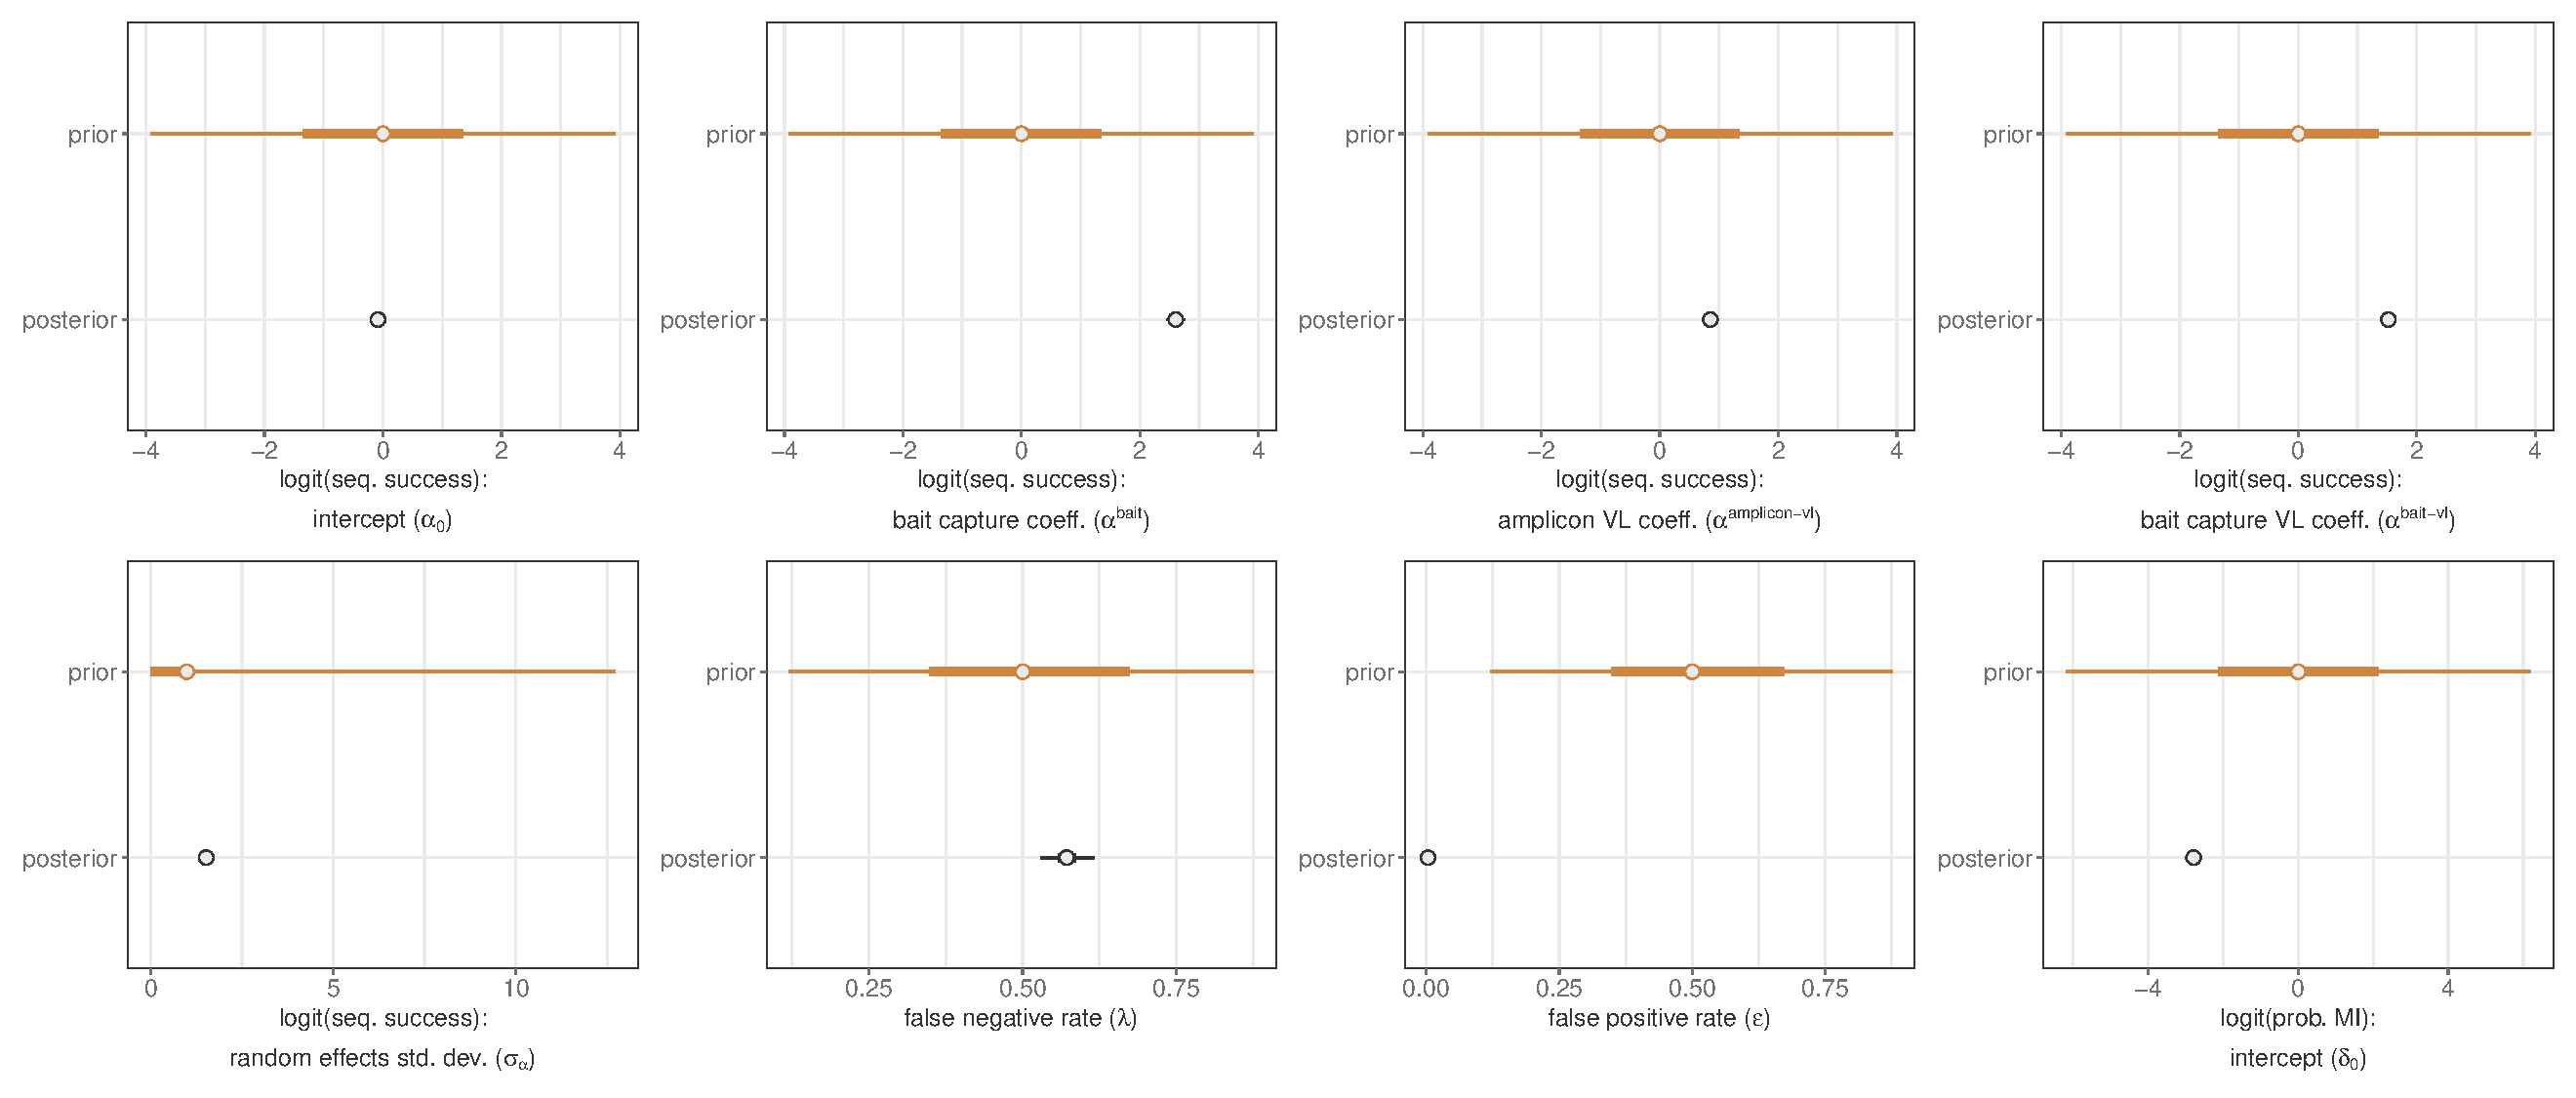
\includegraphics[width=1\textwidth]{../../figures/empirical_full_prior.pdf}}{}
\caption{{\bf Comparison of posterior and prior distributions of parameters in full model fit to deep sequence data generated from \protect \var{empirical_full_n_participant_visits} Rakai Community Cohort Study participants living with viremic HIV.} Median is plotted as the central estimate and horizontal bars extend to the 95\% and 50\% HPD. Some horizontal bars do not extend beyond the central point. Warm-up iterations are excluded. MI = multiple infection. VL = viral load (log\textsubscript{10} copies/mL) standardized to mean = 0 and std. dev = 1. Std. dev. = standard deviation. }
\end{figure}

% empirical comm_type
\begin{figure}[!ht]
 \ifthenelse{\boolean{includefigs}}{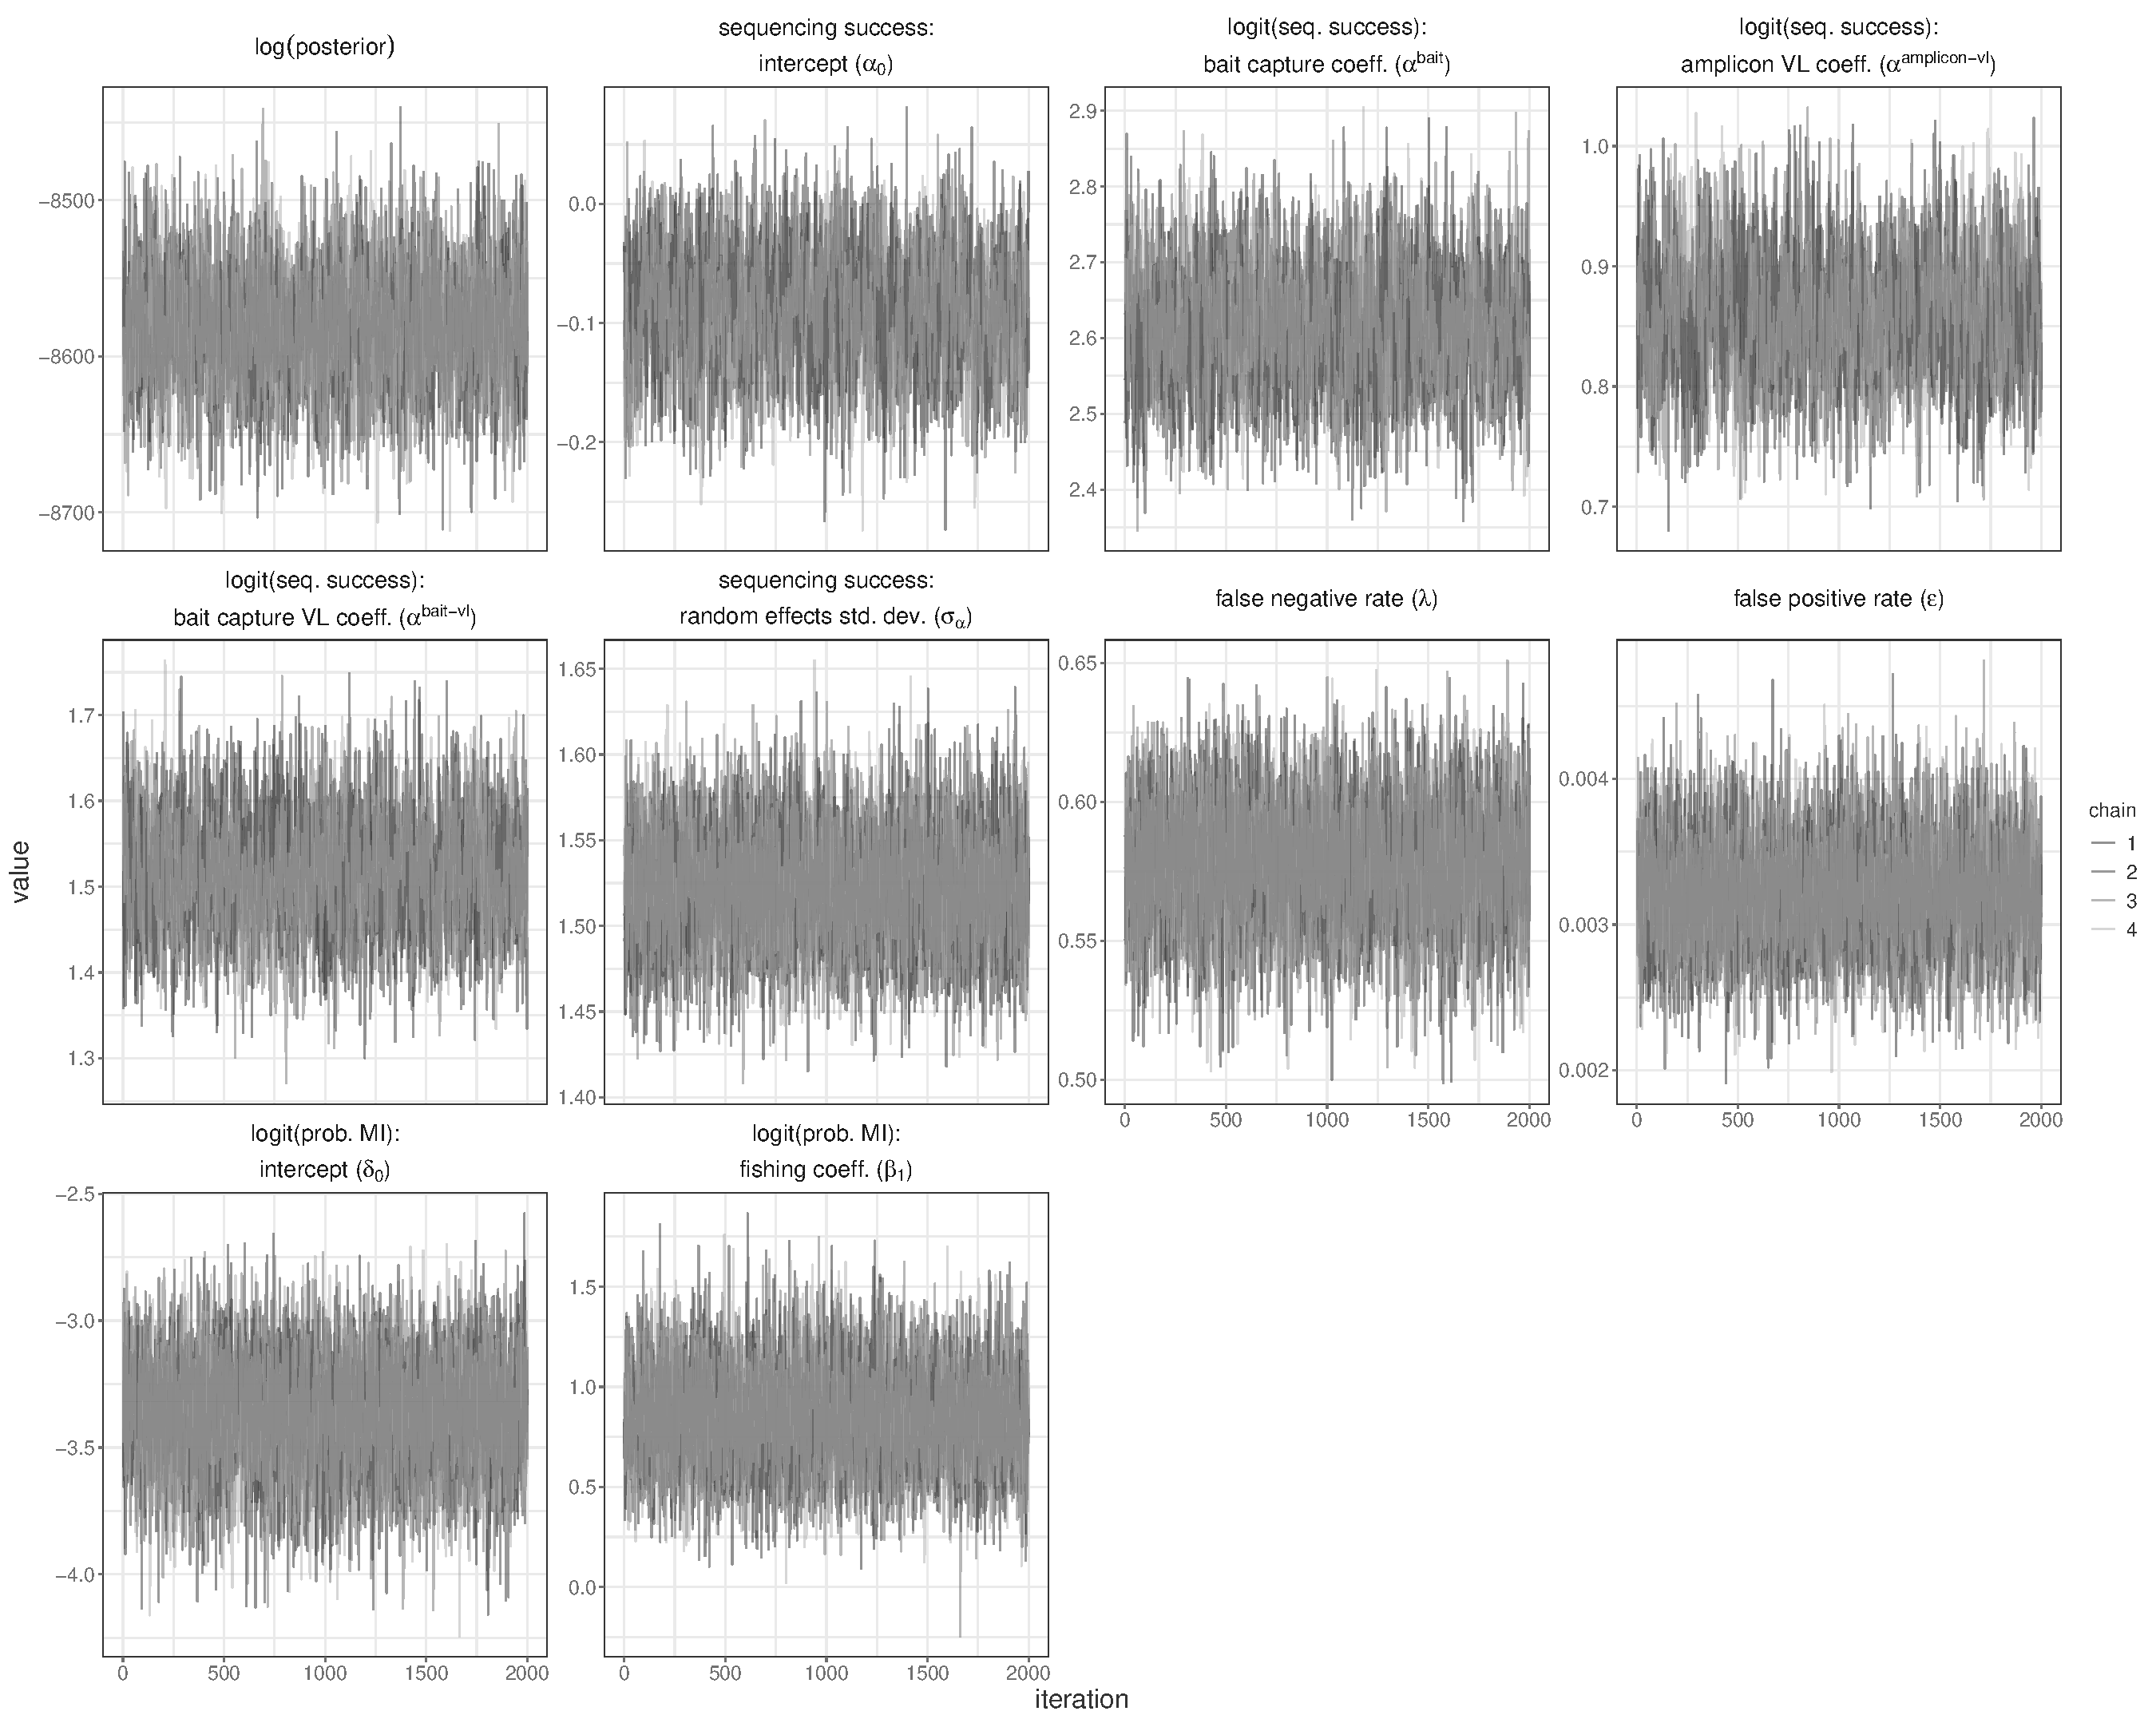
\includegraphics[width=1\textwidth]{../../figures/empirical_commtype_trace.pdf}}{}
\caption{{\bf MCMC trace plots for parameters in extended model with community type as a risk factor fit to deep sequence data generated from \protect \var{empirical_full_n_participant_visits} Rakai Community Cohort Study participants living with viremic HIV.} Independent chains are shown in shades of grey. Warm-up iterations are excluded. MI = multiple infection. VL = viral load (log\textsubscript{10} copies/mL) standardized to mean = 0 and std. dev = 1. Std. dev. = standard deviation. }
\end{figure}

\begin{figure}[!ht]
 \ifthenelse{\boolean{includefigs}}{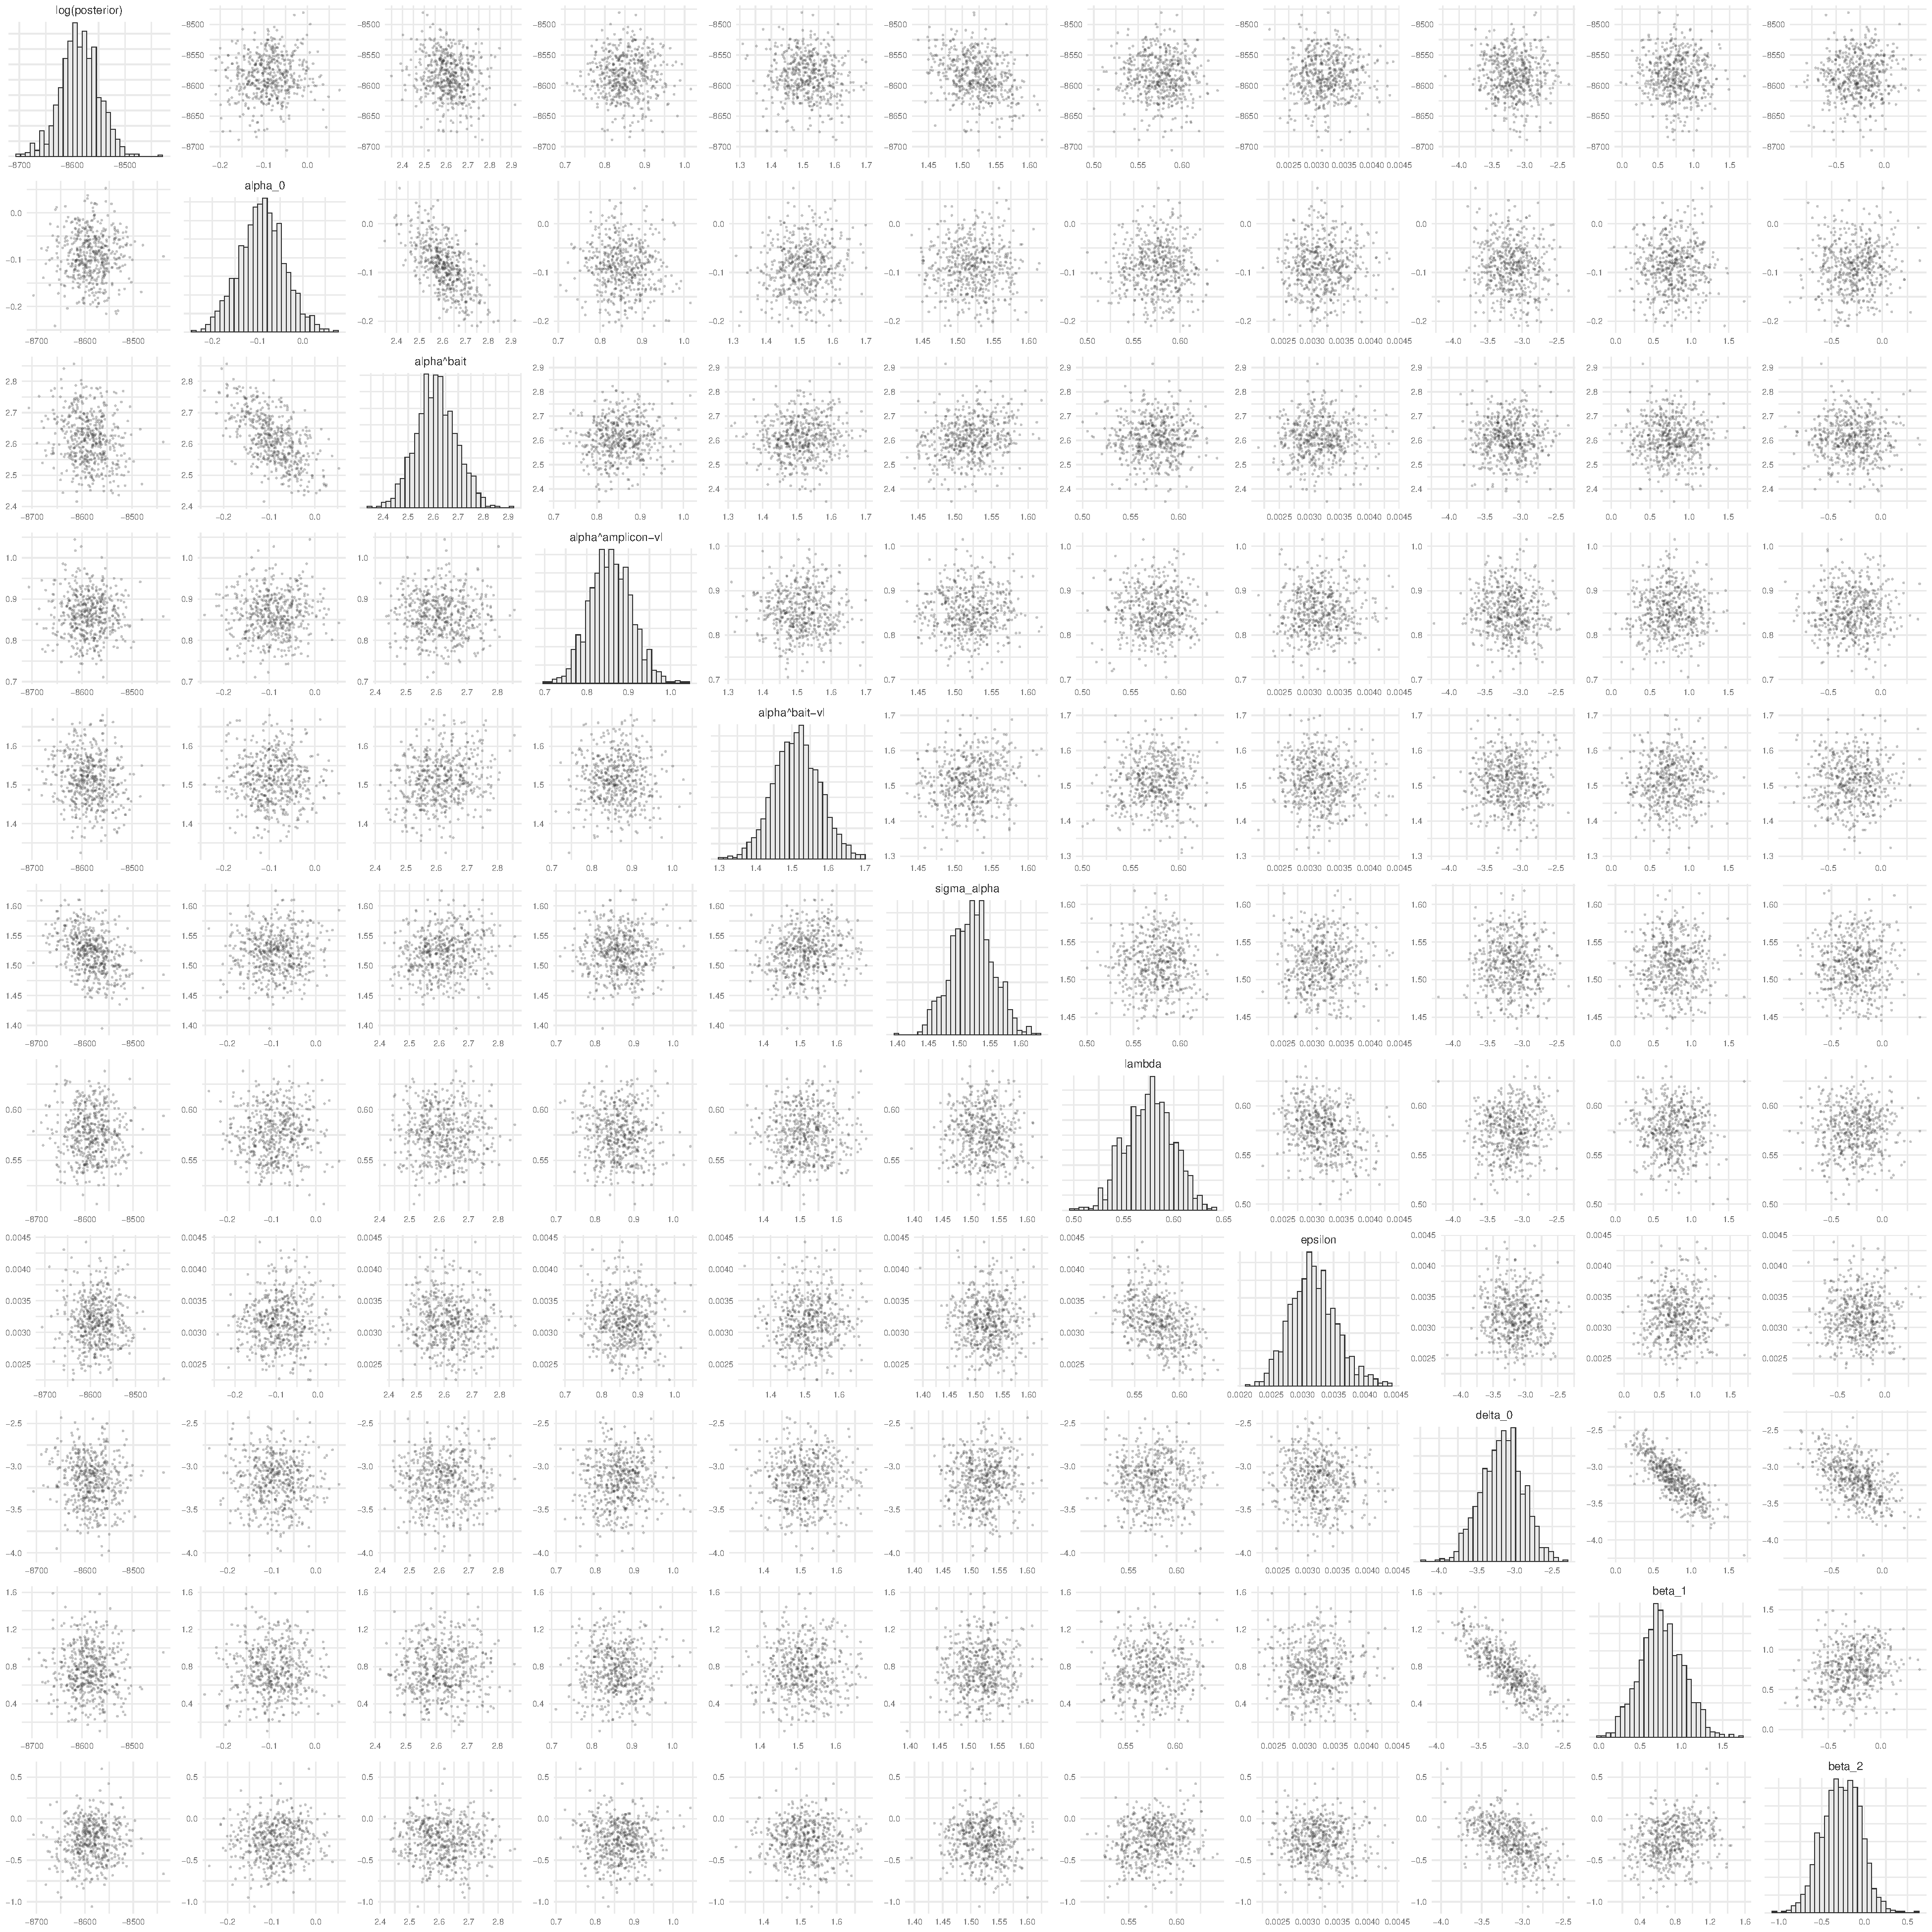
\includegraphics[width=1\textwidth]{../../figures/empirical_commtype_pairs.pdf}}{}
\caption{{\bf MCMC pairs plots for parameters in extended model with community type as a risk factor fit to deep sequence data generated from \protect \var{empirical_full_n_participant_visits} Rakai Community Cohort Study participants living with viremic HIV.} Independent chains are shown in shades of grey. Warm-up iterations are excluded. Includes a sample of 250 iterations per chain. MI = multiple infection. }
\end{figure}

\begin{figure}[!ht]
 \ifthenelse{\boolean{includefigs}}{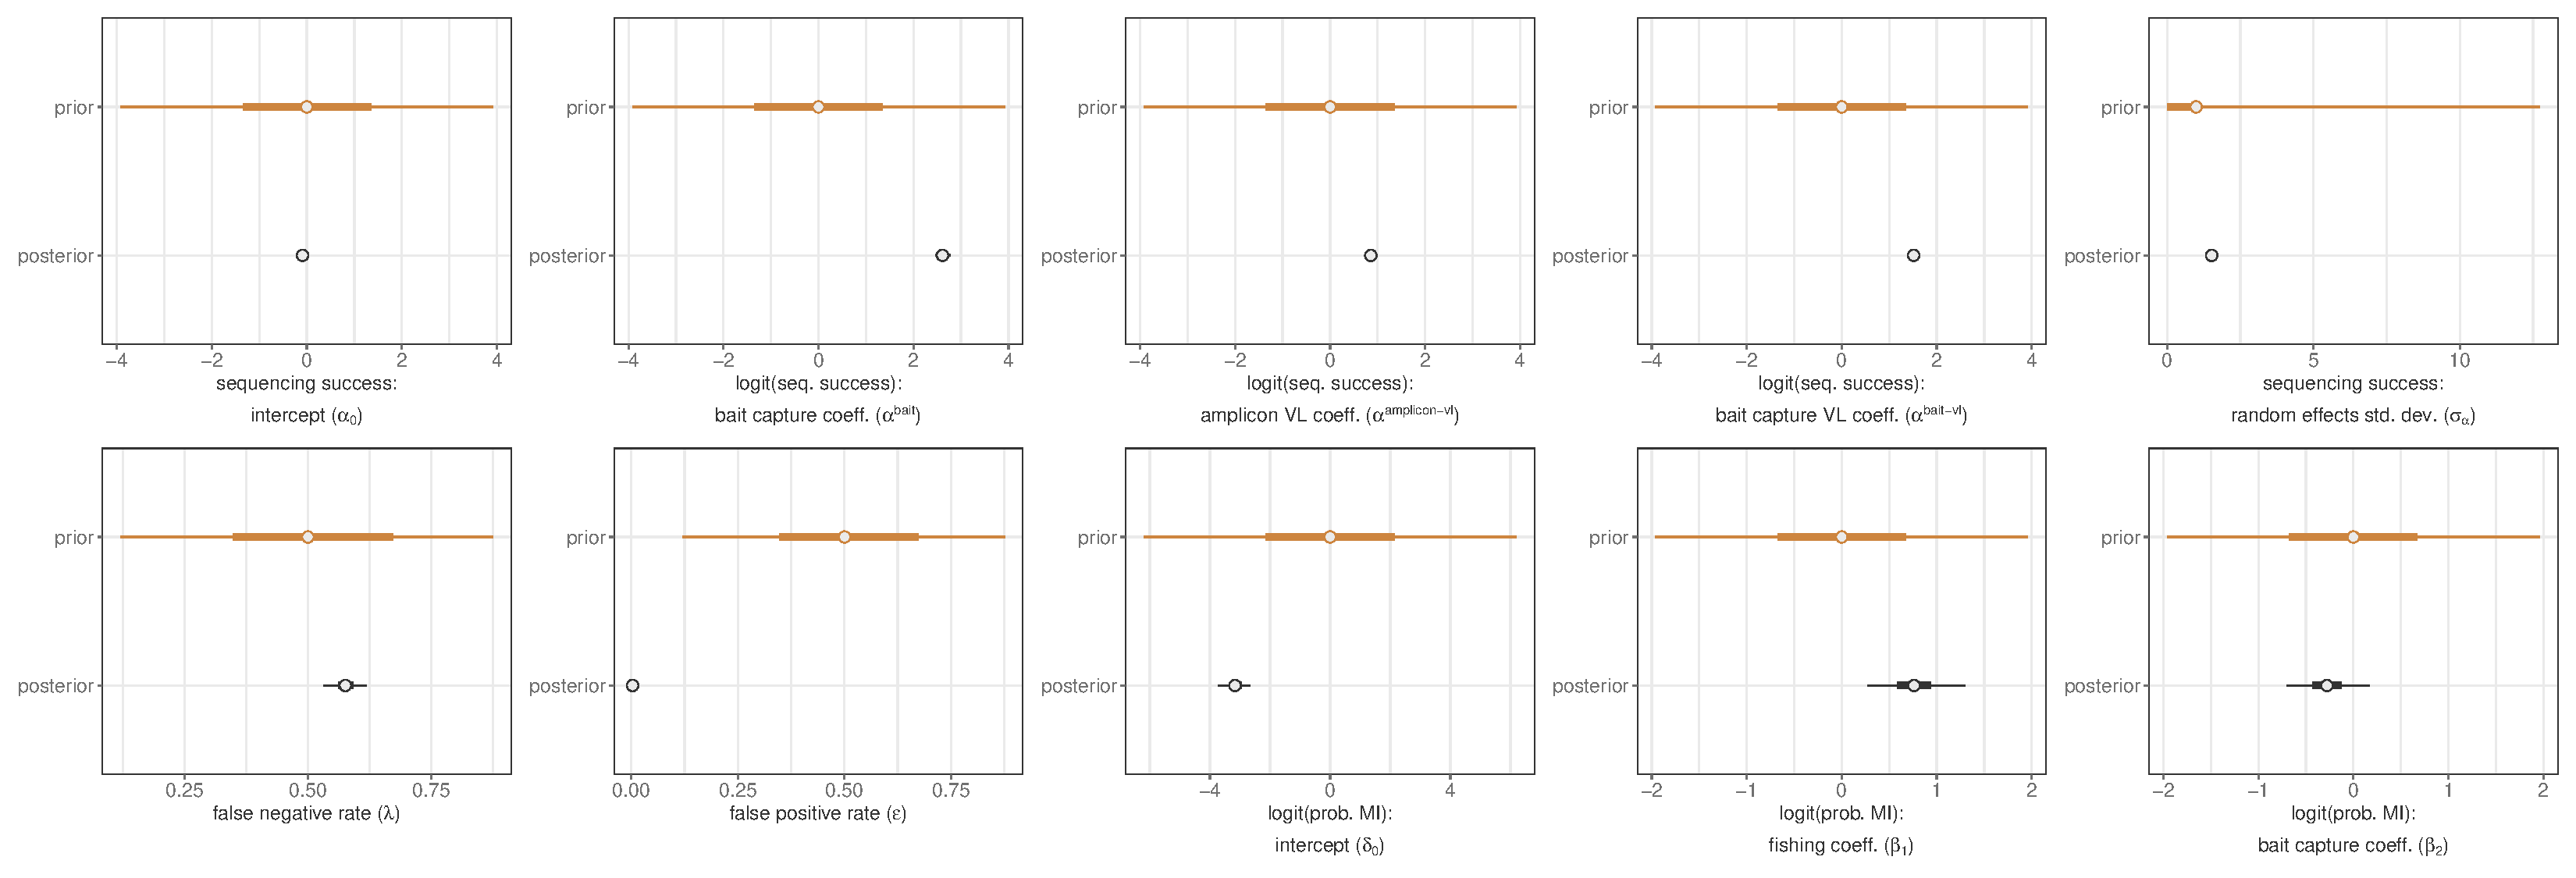
\includegraphics[width=1\textwidth]{../../figures/empirical_commtype_prior.pdf}}{}
\caption{{\bf Comparison of posterior and prior distributions of parameters in extended model with community type as a risk factor fit to deep sequence data generated from \protect \var{empirical_full_n_participant_visits} Rakai Community Cohort Study participants living with viremic HIV.} Median is plotted as the central estimate and horizontal bars extend to the 95\% and 50\% HPD. Some horizontal bars do not extend beyond the central point. Warm-up iterations are excluded. MI = multiple infection. VL = viral load (log\textsubscript{10} copies/mL) standardized to mean = 0 and std. dev = 1. Std. dev. = standard deviation. }
\end{figure}

% empirical seq_tech
\begin{figure}[!ht]
 \ifthenelse{\boolean{includefigs}}{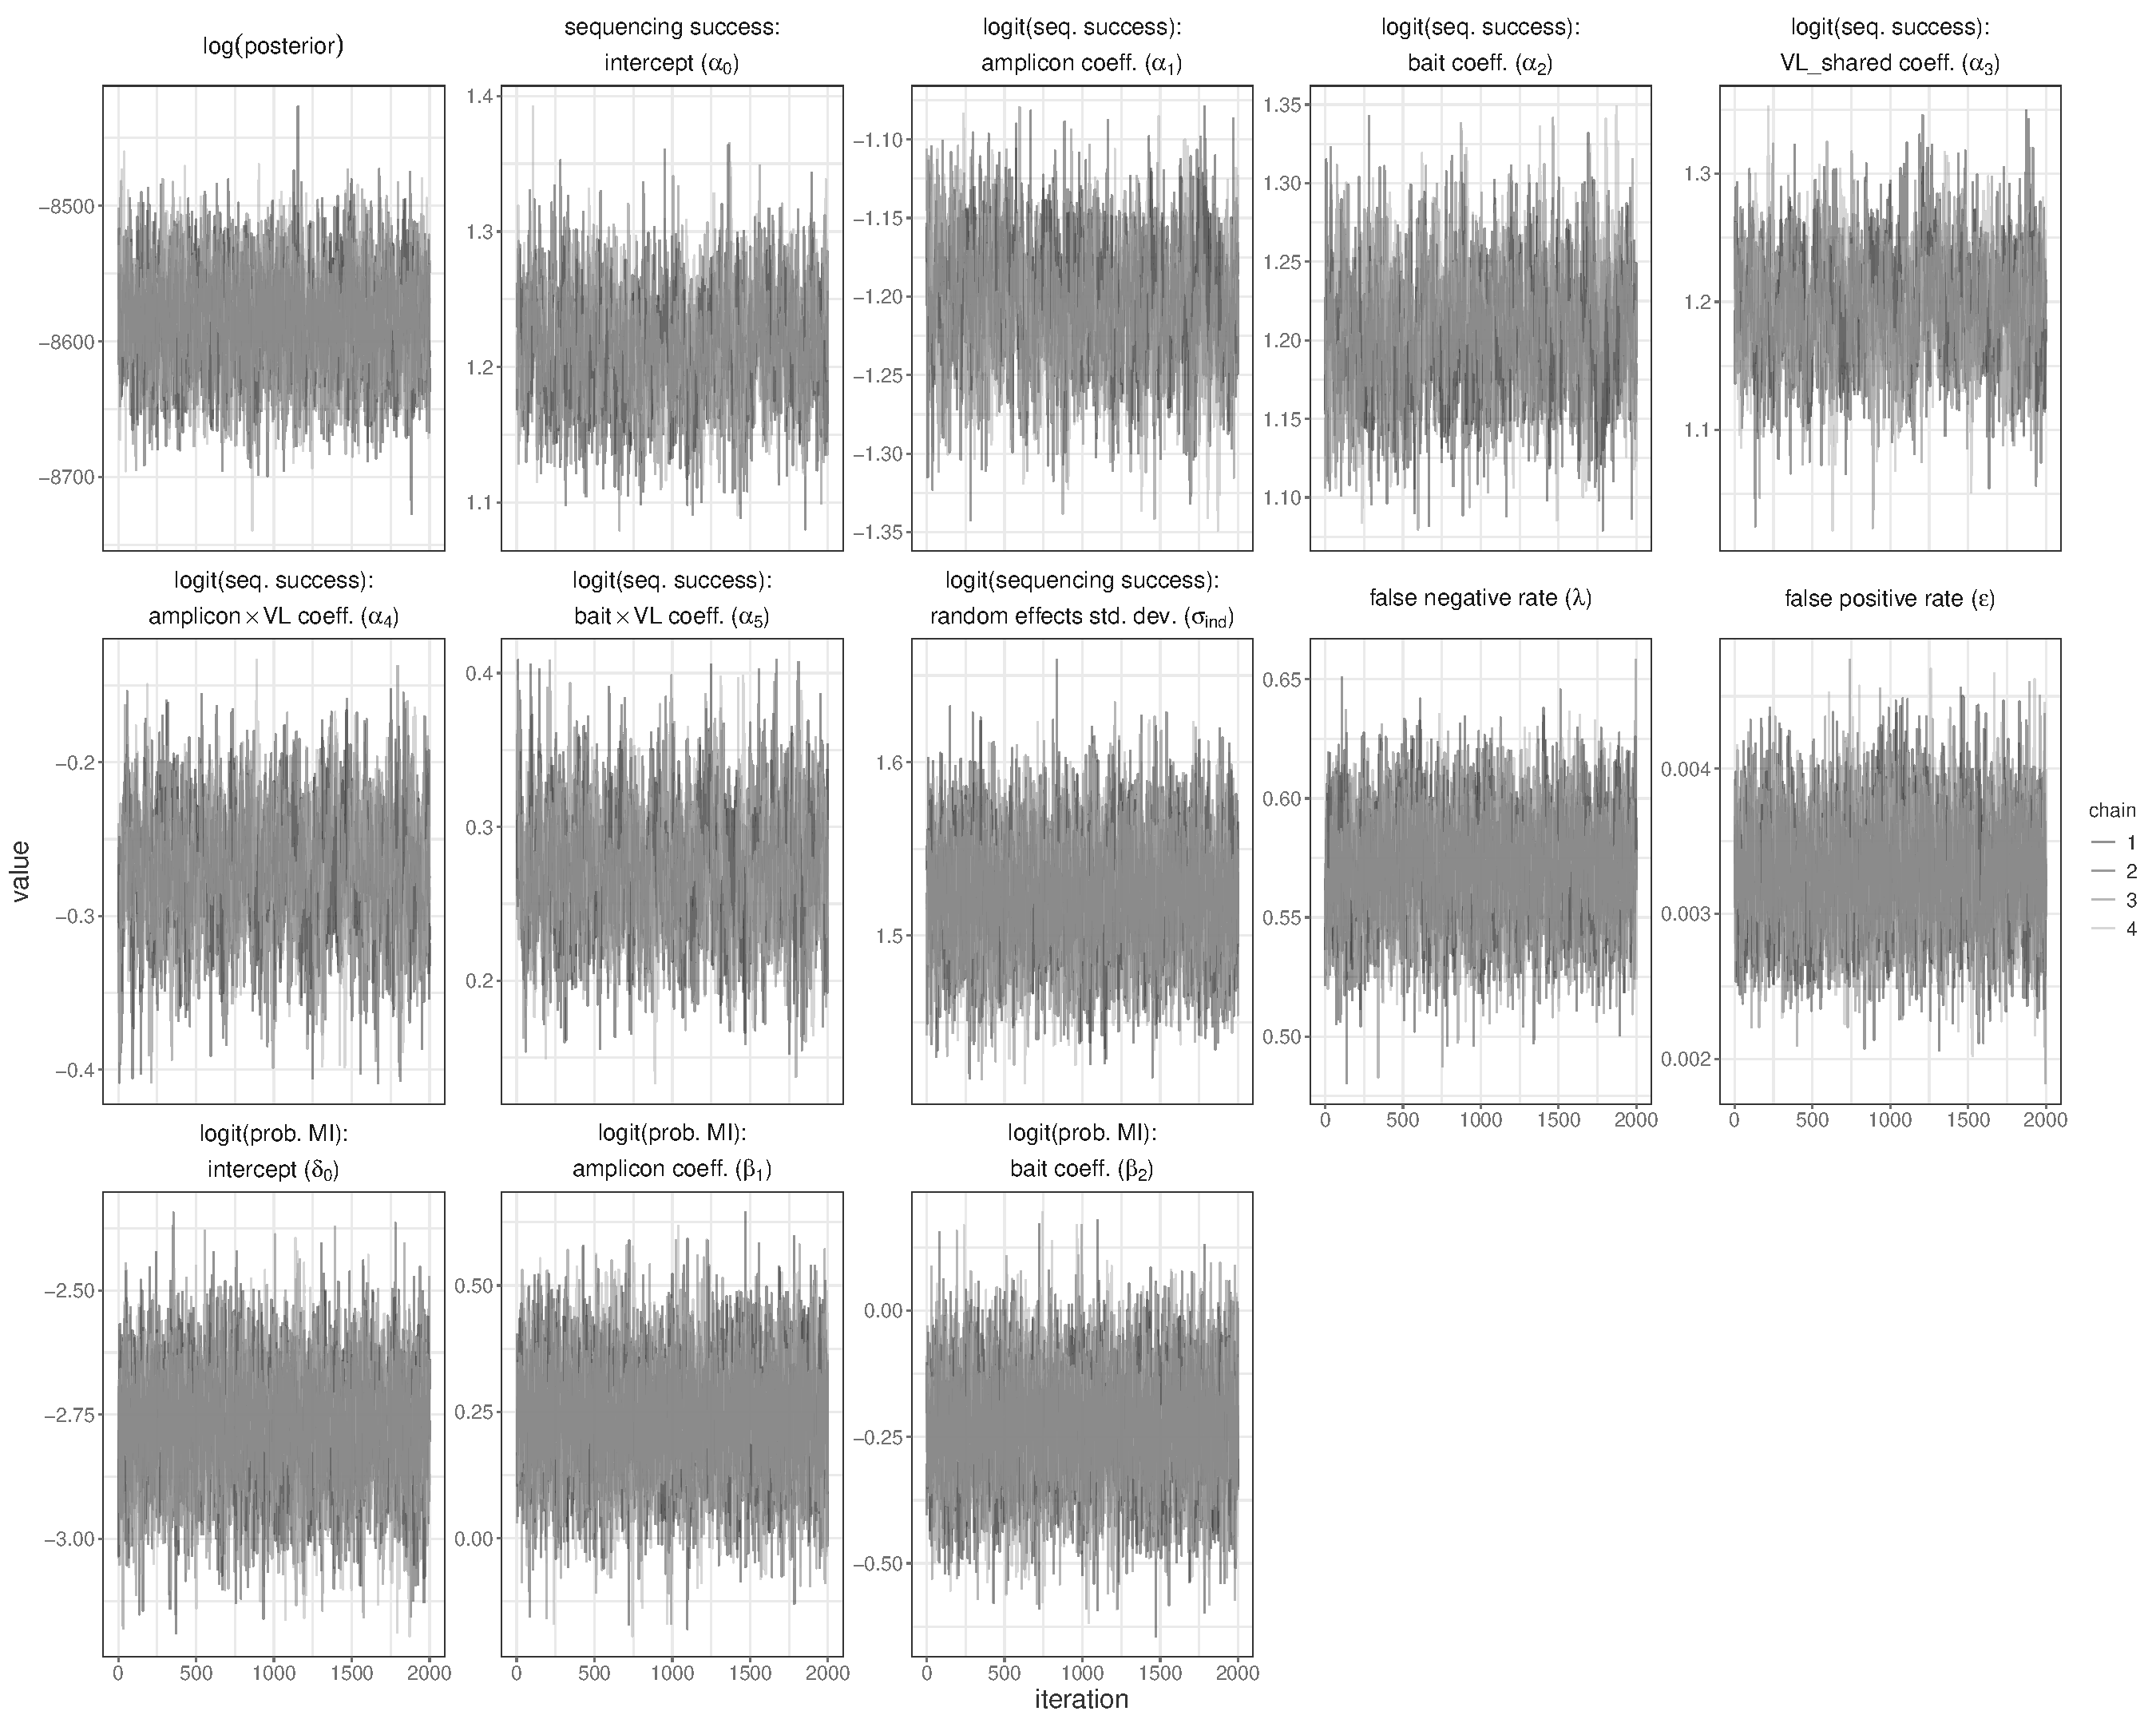
\includegraphics[width=1\textwidth]{../../figures/empirical_seqtech_trace.pdf}}{}
\caption{{\bf MCMC trace plots for parameters in extended model with deep-sequencing protocol as a risk factor fit to deep sequence data generated from \protect \var{empirical_full_n_participant_visits} Rakai Community Cohort Study participants living with viremic HIV.} Independent chains are shown in shades of grey. Warm-up iterations are excluded. MI = multiple infection. VL = viral load (log\textsubscript{10} copies/mL) standardized to mean = 0 and std. dev = 1. Std. dev. = standard deviation. }
\end{figure}

\begin{figure}[!ht]
 \ifthenelse{\boolean{includefigs}}{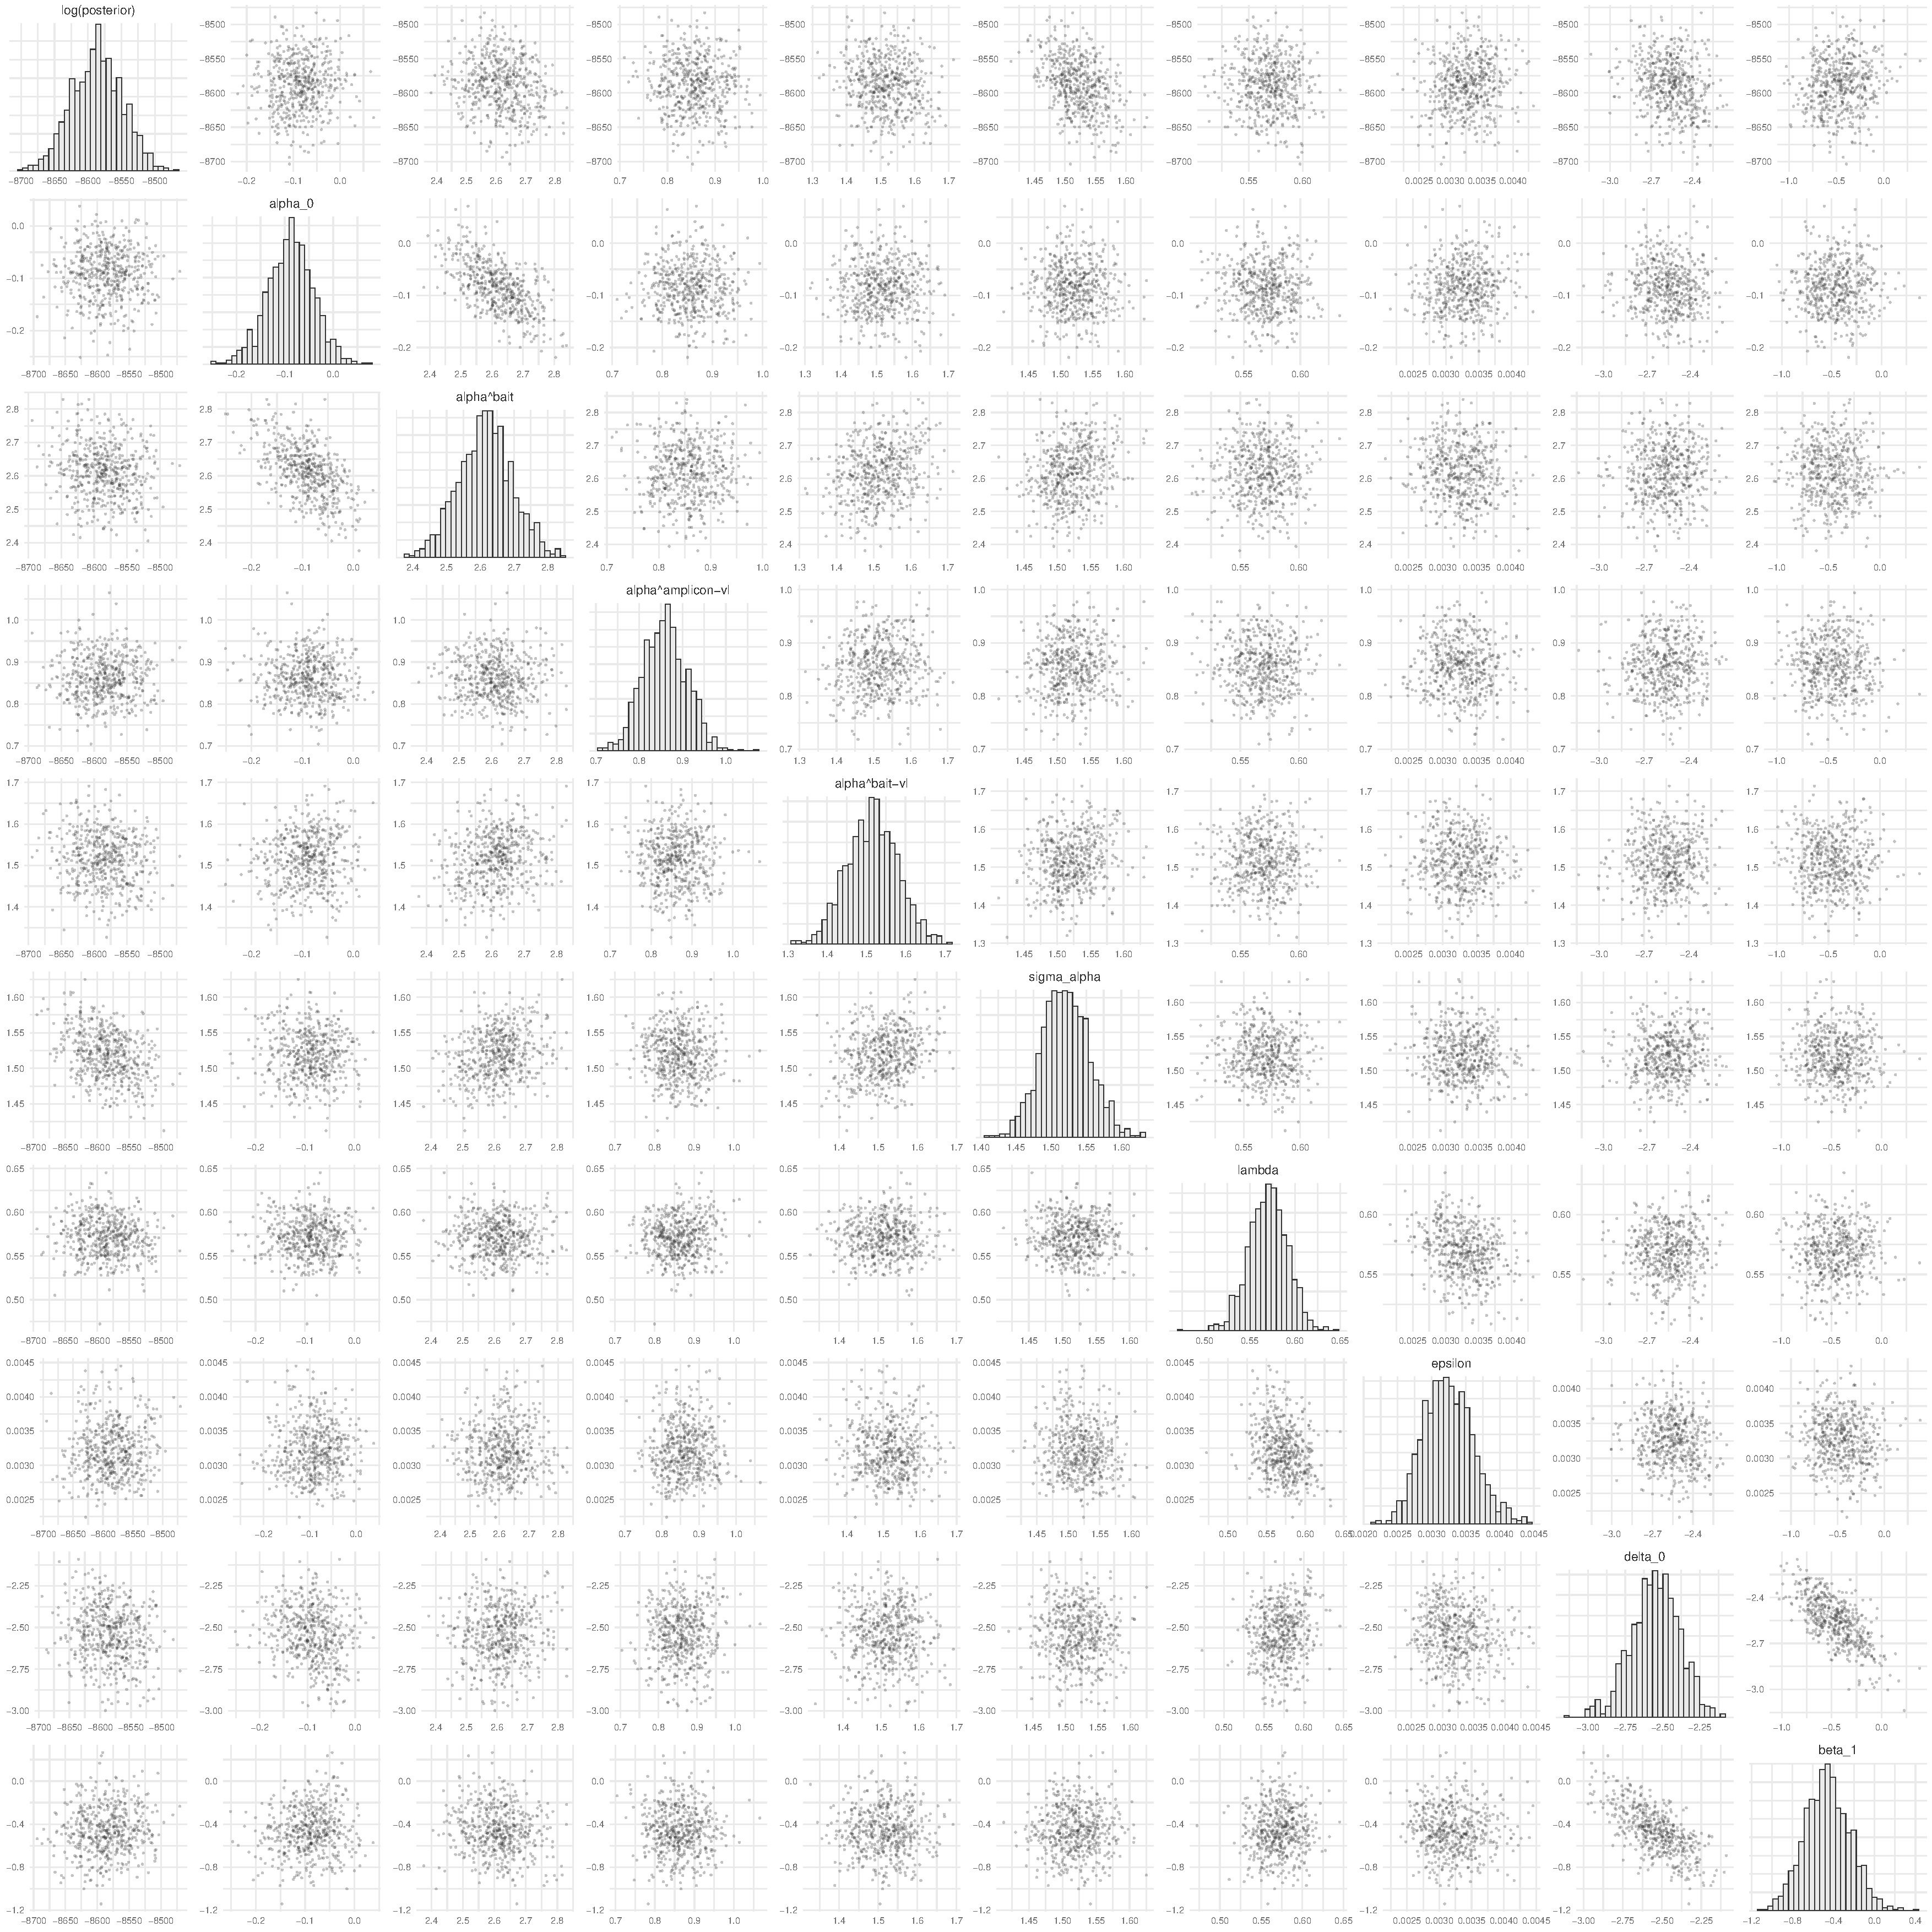
\includegraphics[width=1\textwidth]{../../figures/empirical_seqtech_pairs.pdf}}{}
\caption{{\bf MCMC pairs plots for parameters in extended model withdeep-sequencing protocol as a risk factor fit to deep sequence data generated from \protect \var{empirical_full_n_participant_visits} Rakai Community Cohort Study participants living with viremic HIV.} Independent chains are shown in shades of grey. Warm-up iterations are excluded. Includes a sample of 250 iterations per chain. MI = multiple infection. }
\end{figure}

\begin{figure}[!ht]
 \ifthenelse{\boolean{includefigs}}{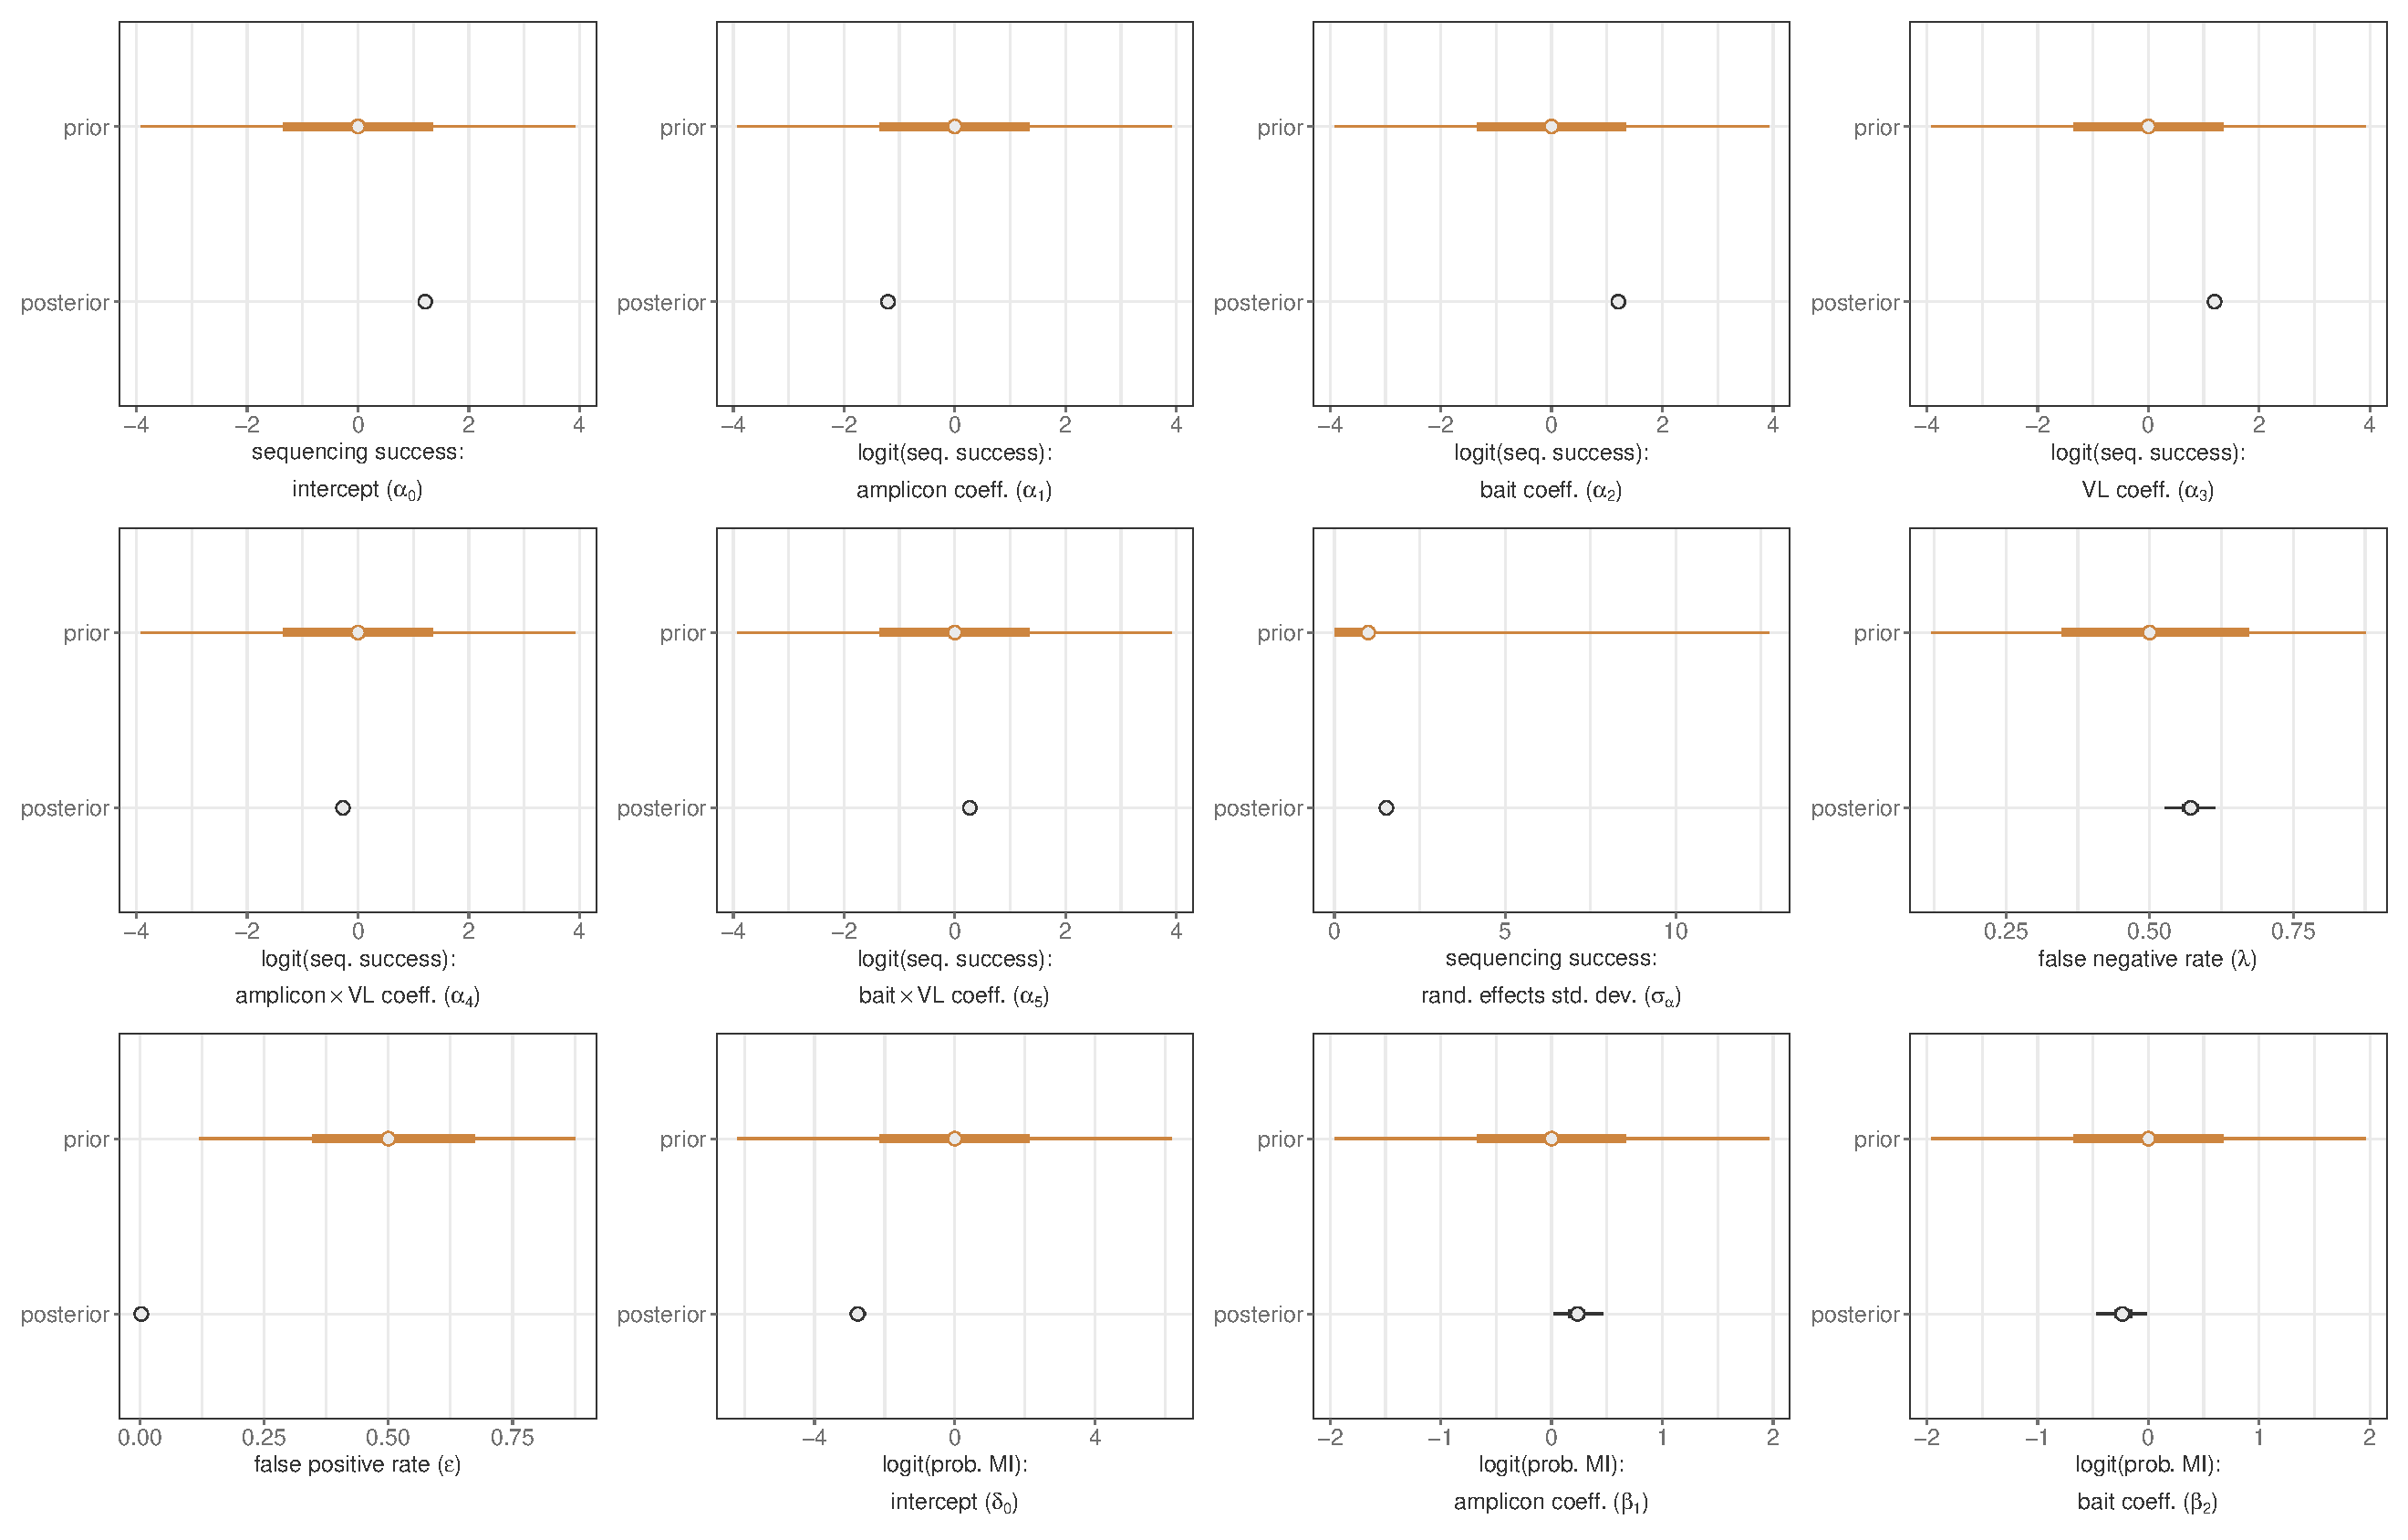
\includegraphics[width=1\textwidth]{../../figures/empirical_seqtech_prior.pdf}}{}
\caption{{\bf Comparison of posterior and prior distributions of parameters in extended model with sequencing technology as a risk factor fit to deep sequence data generated from \protect \var{empirical_full_n_participant_visits} Rakai Community Cohort Study participants living with viremic HIV.} Median is plotted as the central estimate and horizontal bars extend to the 95\% and 50\% HPD. Some horizontal bars do not extend beyond the central point. Warm-up iterations are excluded. MI = multiple infection. VL = viral load (log\textsubscript{10} copies/mL) standardized to mean = 0 and std. dev = 1. Std. dev. = standard deviation. }
\end{figure}


% empirical seq_tech_comm_type
\begin{figure}[!ht]
 \ifthenelse{\boolean{includefigs}}{\includegraphics[width=1\textwidth]{../../figures/empirical_seqtech_comm_trace.pdf}}{}
\caption{{\bf MCMC trace plots for parameters in extended model with deep-sequencing protocol and community type as a risk factor fit to deep sequence data generated from \protect \var{empirical_full_n_participant_visits} Rakai Community Cohort Study participants living with viremic HIV.} Independent chains are shown in shades of grey. Warm-up iterations are excluded. MI = multiple infection. VL = viral load (log\textsubscript{10} copies/mL) standardized to mean = 0 and std. dev = 1. Std. dev. = standard deviation. }
\end{figure}

\begin{figure}[!ht]
 \ifthenelse{\boolean{includefigs}}{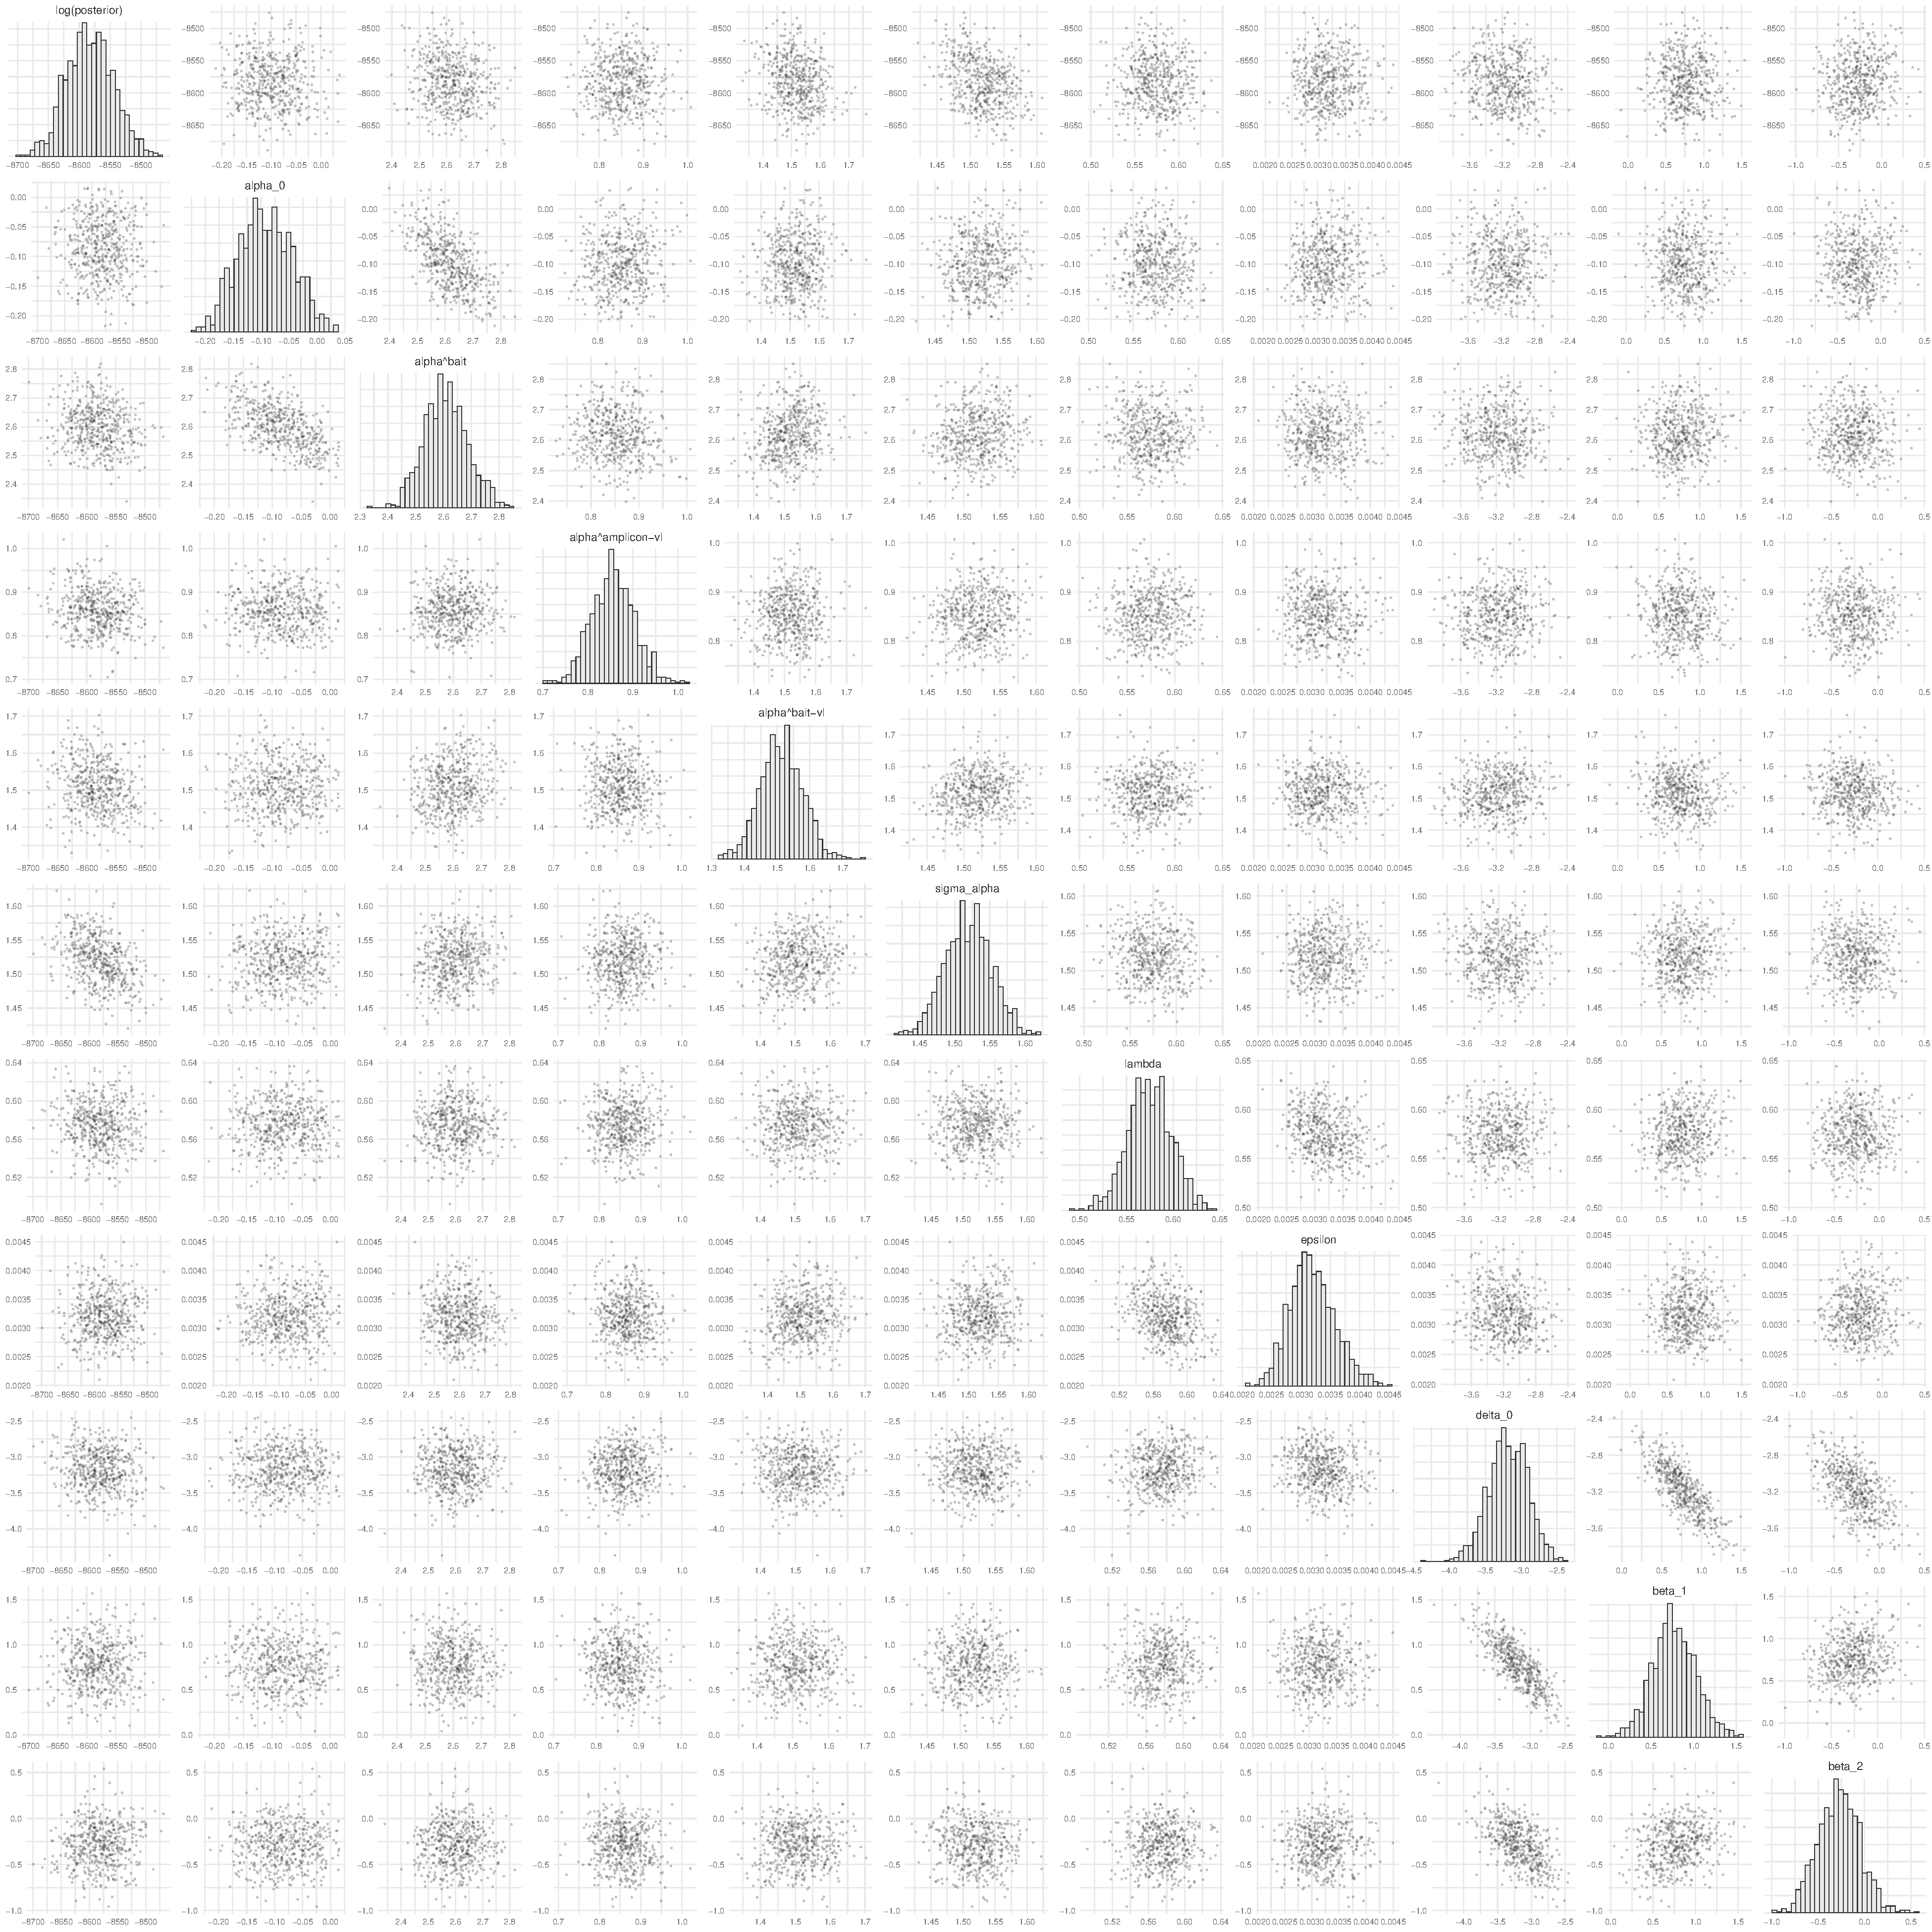
\includegraphics[width=1\textwidth]{../../figures/empirical_seqtech_comm_pairs.pdf}}{}
\caption{{\bf MCMC pairs plots for parameters in extended model withdeep-sequencing protocol and community type as a risk factor fit to deep sequence data generated from \protect \var{empirical_full_n_participant_visits} Rakai Community Cohort Study participants living with viremic HIV.} Independent chains are shown in shades of grey. Warm-up iterations are excluded. Includes a sample of 250 iterations per chain. MI = multiple infection. }
\end{figure}

\begin{figure}[!ht]
 \ifthenelse{\boolean{includefigs}}{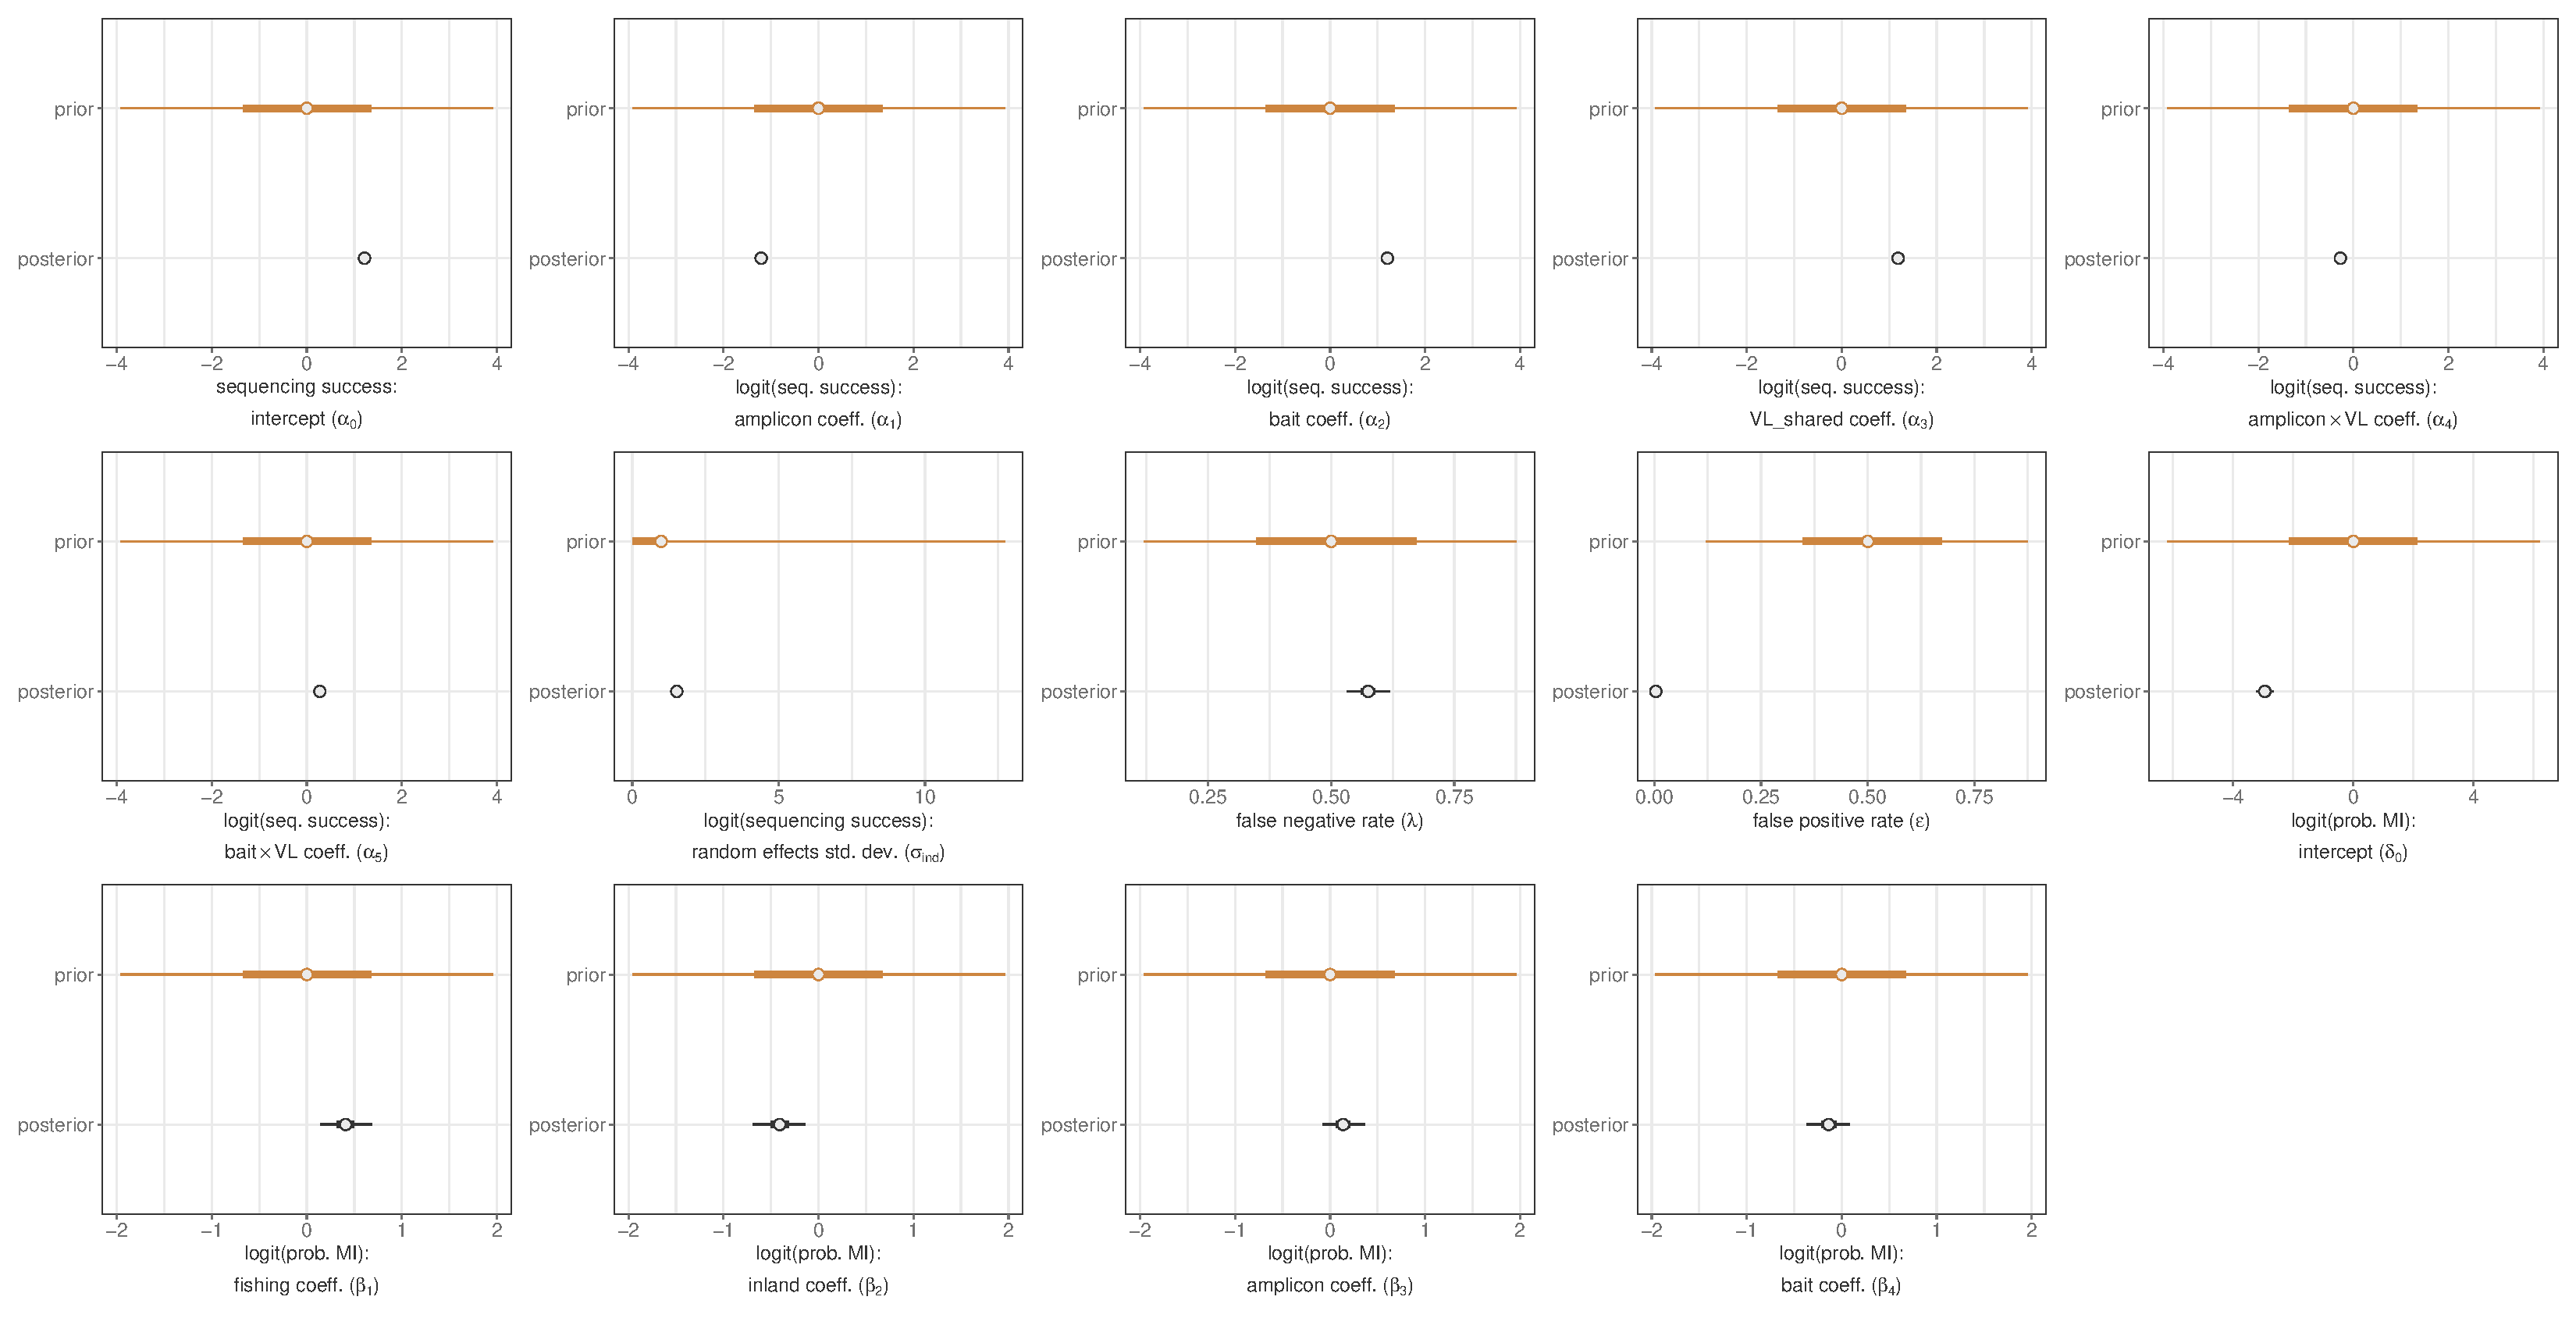
\includegraphics[width=1\textwidth]{../../figures/empirical_seqtech_comm_prior.pdf}}{}
\caption{{\bf Comparison of posterior and prior distributions of parameters in extended model with sequencing technology and community type as a risk factor fit to deep sequence data generated from \protect \var{empirical_full_n_participant_visits} Rakai Community Cohort Study participants living with viremic HIV.} Median is plotted as the central estimate and horizontal bars extend to the 95\% and 50\% HPD. Some horizontal bars do not extend beyond the central point. Warm-up iterations are excluded. MI = multiple infection. VL = viral load (log\textsubscript{10} copies/mL) standardized to mean = 0 and std. dev = 1. Std. dev. = standard deviation. }
\end{figure}


% empirical sexpever 
\begin{figure}[!ht]
 \ifthenelse{\boolean{includefigs}}{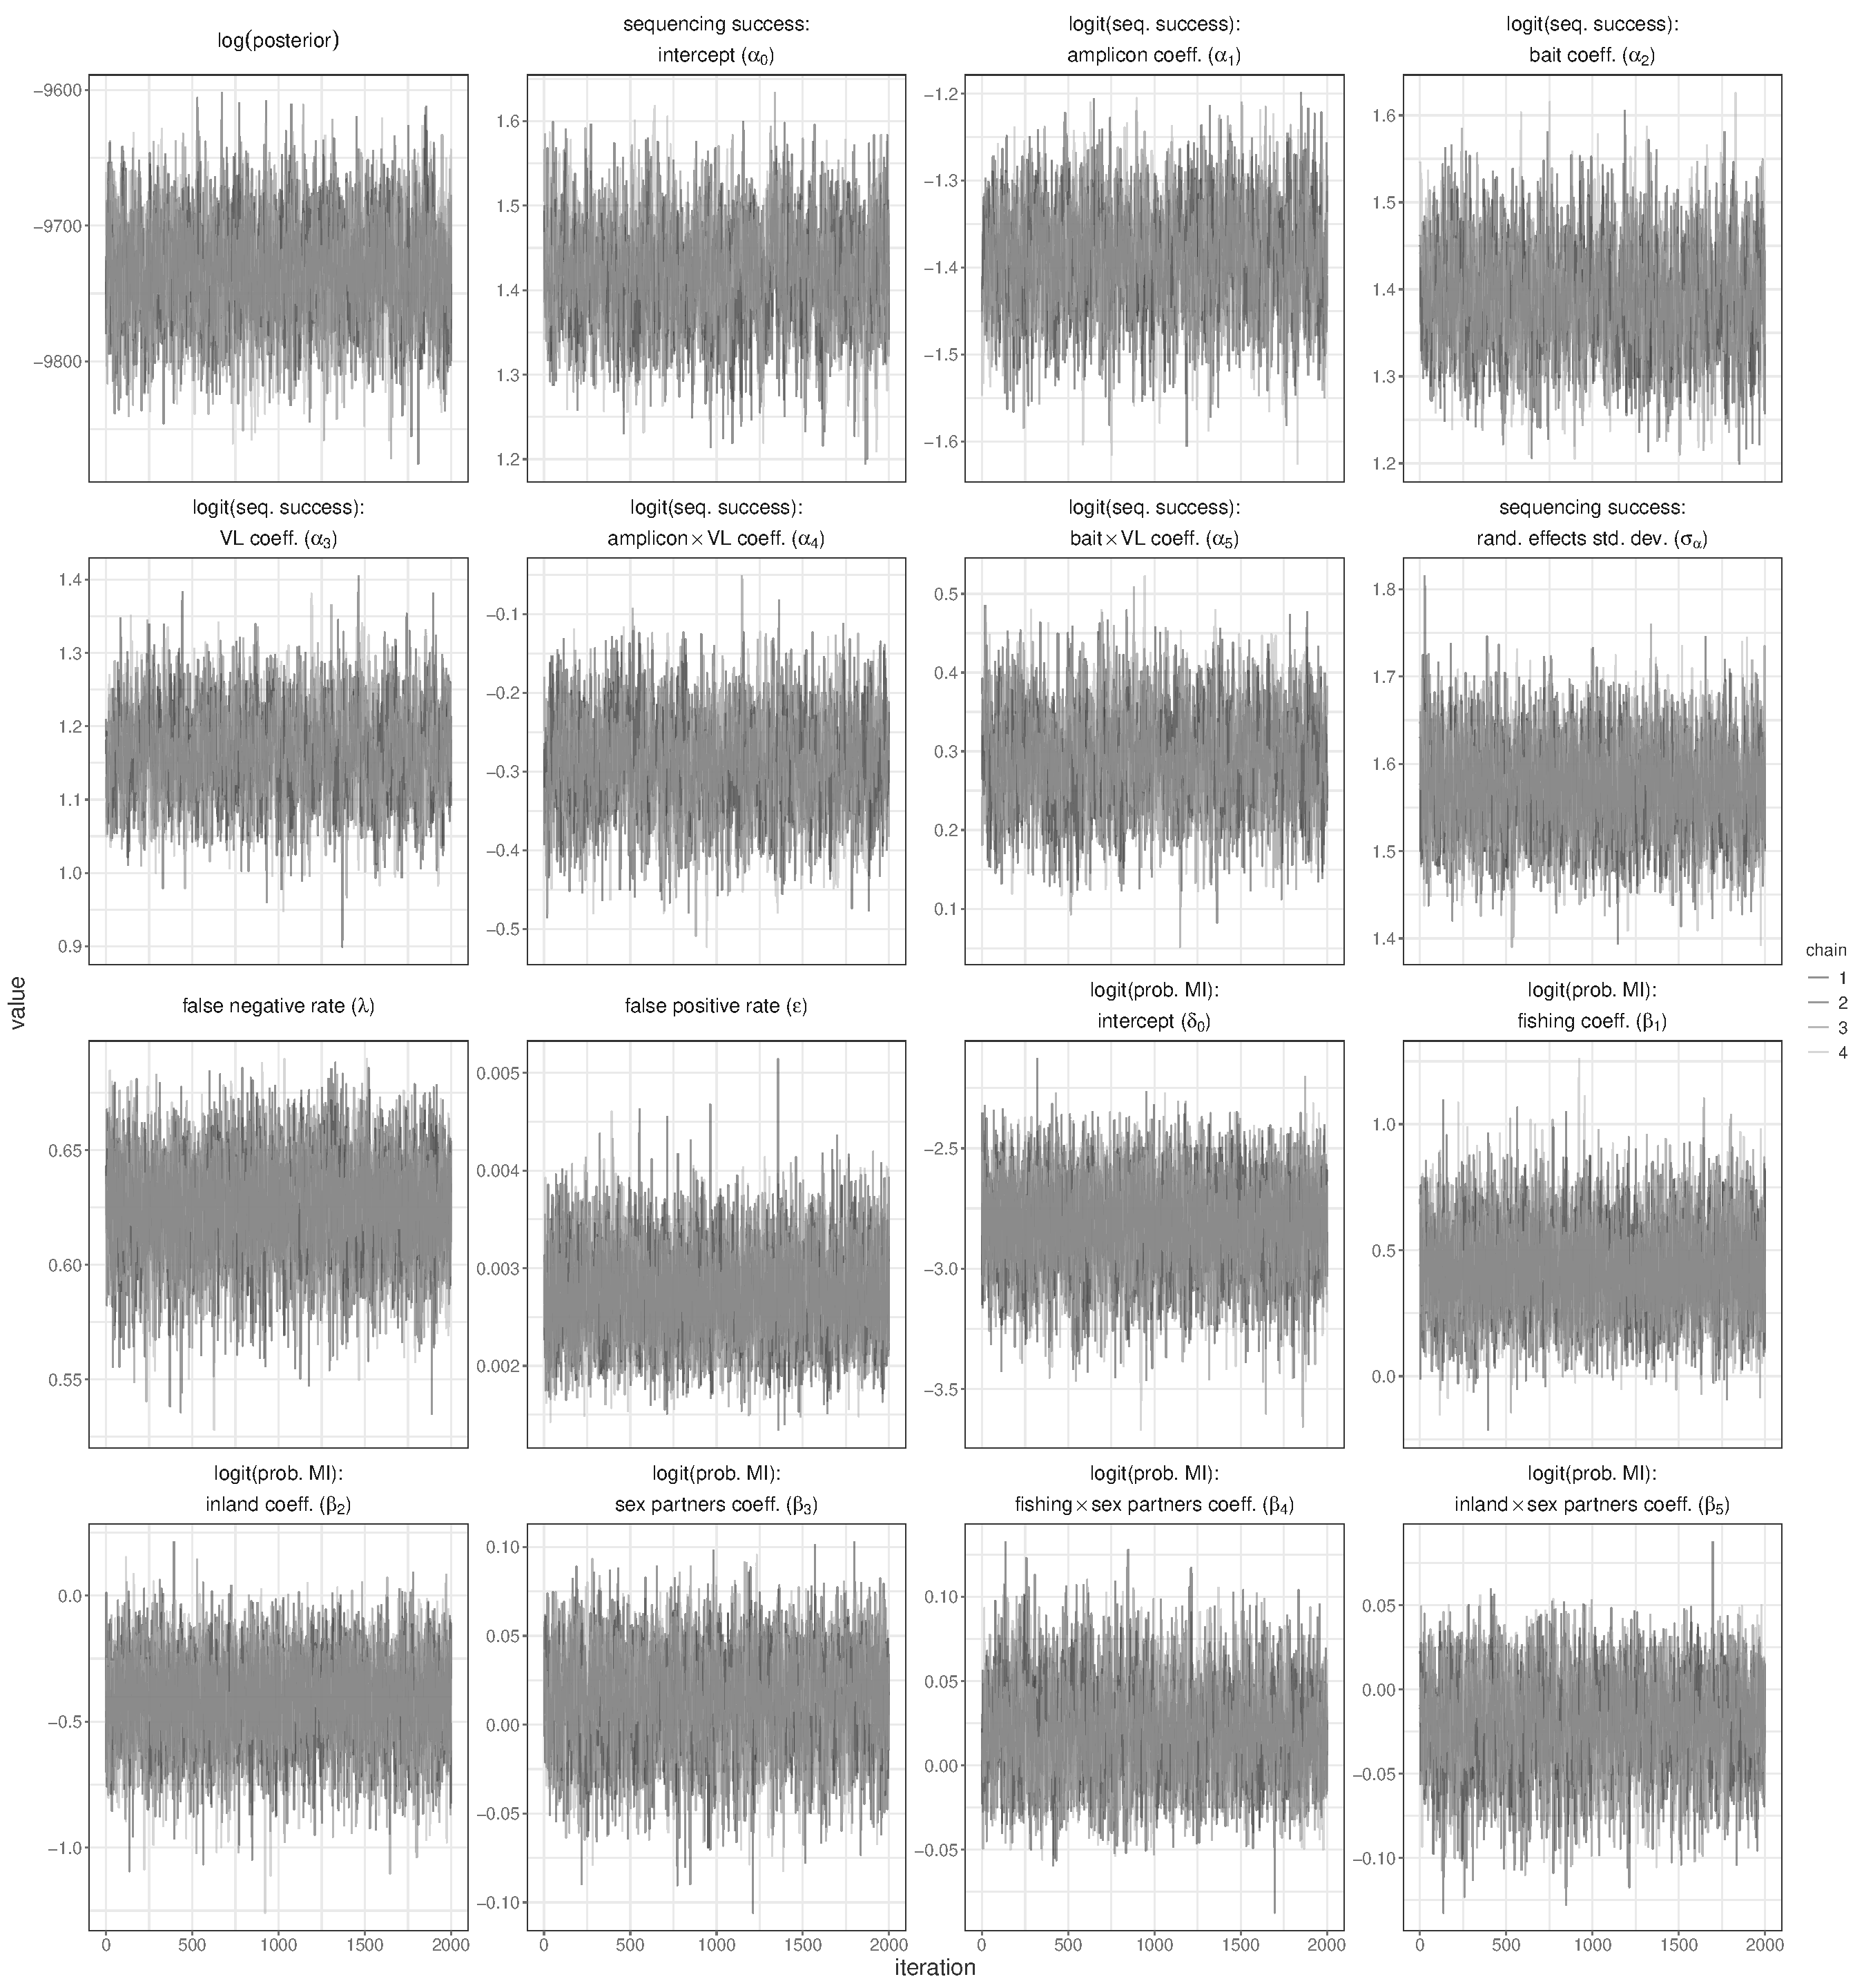
\includegraphics[width=1\textwidth]{../../figures/empirical_sexpever_men_trace.pdf}}{}
\caption{{\bf MCMC trace plots for parameters in extended model with community type and lifetime sex partners as a risk factor for harboring multiple infections fit to deep sequence data generated from \protect \var{empirical_sexpever_men_n_participant_visits} men living with viremic HIV who participated in the Rakai Community Cohort Study.} Independent chains are shown in shades of grey. Warm-up iterations are excluded. MI = multiple infection. VL = viral load (log\textsubscript{10} copies/mL) standardized to mean = 0 and std. dev = 1. Std. dev. = standard deviation.}
\end{figure}

\begin{figure}[!ht]
 \ifthenelse{\boolean{includefigs}}{\includegraphics[width=1\textwidth]{../../figures/empirical_sexpever_men_pairs.pdf}}{}
\caption{{\bf MCMC  pairs plots for parameters in extended model with community type and lifetime sex partners as a risk factor for harboring multiple infections fit to deep sequence data generated from \protect \var{empirical_sexpever_men_n_participant_visits} men living with viremic HIV who participated in the Rakai Community Cohort Study.} Independent chains are shown in shades of grey. Warm-up iterations are excluded. Includes a sample of 250 iterations per chain. MI = multiple infection. }
\end{figure}

\begin{figure}[!ht]
 \ifthenelse{\boolean{includefigs}}{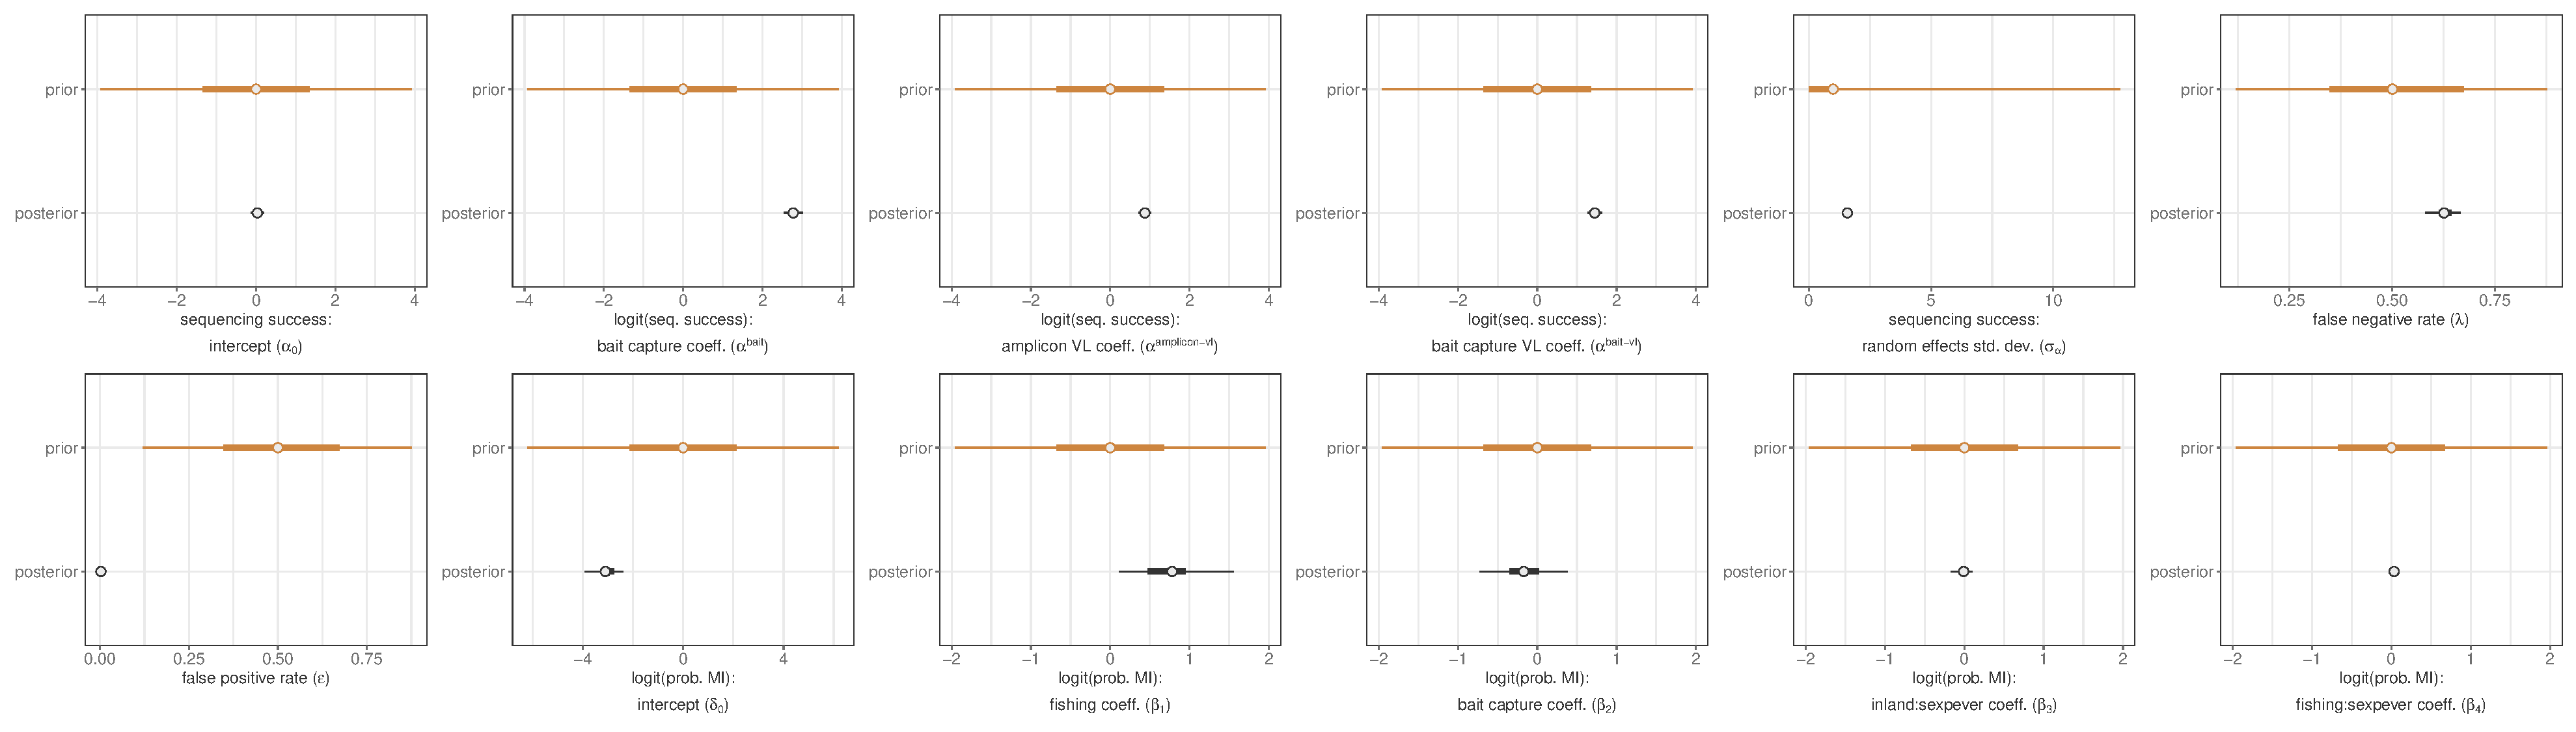
\includegraphics[width=1\textwidth]{../../figures/empirical_sexpever_men_prior.pdf}}{}
\caption{{\bf Comparison of posterior and prior distributions of parameters in extended model with sequencing technology as a risk factor fit to deep sequence data generated from \protect \var{empirical_sexpever_men_n_participant_visits} Rakai Community Cohort Study participants living with viremic HIV.} Median is plotted as the central estimate and horizontal bars extend to the 95\% and 50\% HPD. Some horizontal bars do not extend beyond the central point. Warm-up iterations are excluded. MI = multiple infection. VL = viral load (log\textsubscript{10} copies/mL) standardized to mean = 0 and std. dev = 1. Std. dev. = standard deviation. }
\end{figure}

% empirical var select 
\begin{figure}[!ht]
 \ifthenelse{\boolean{includefigs}}{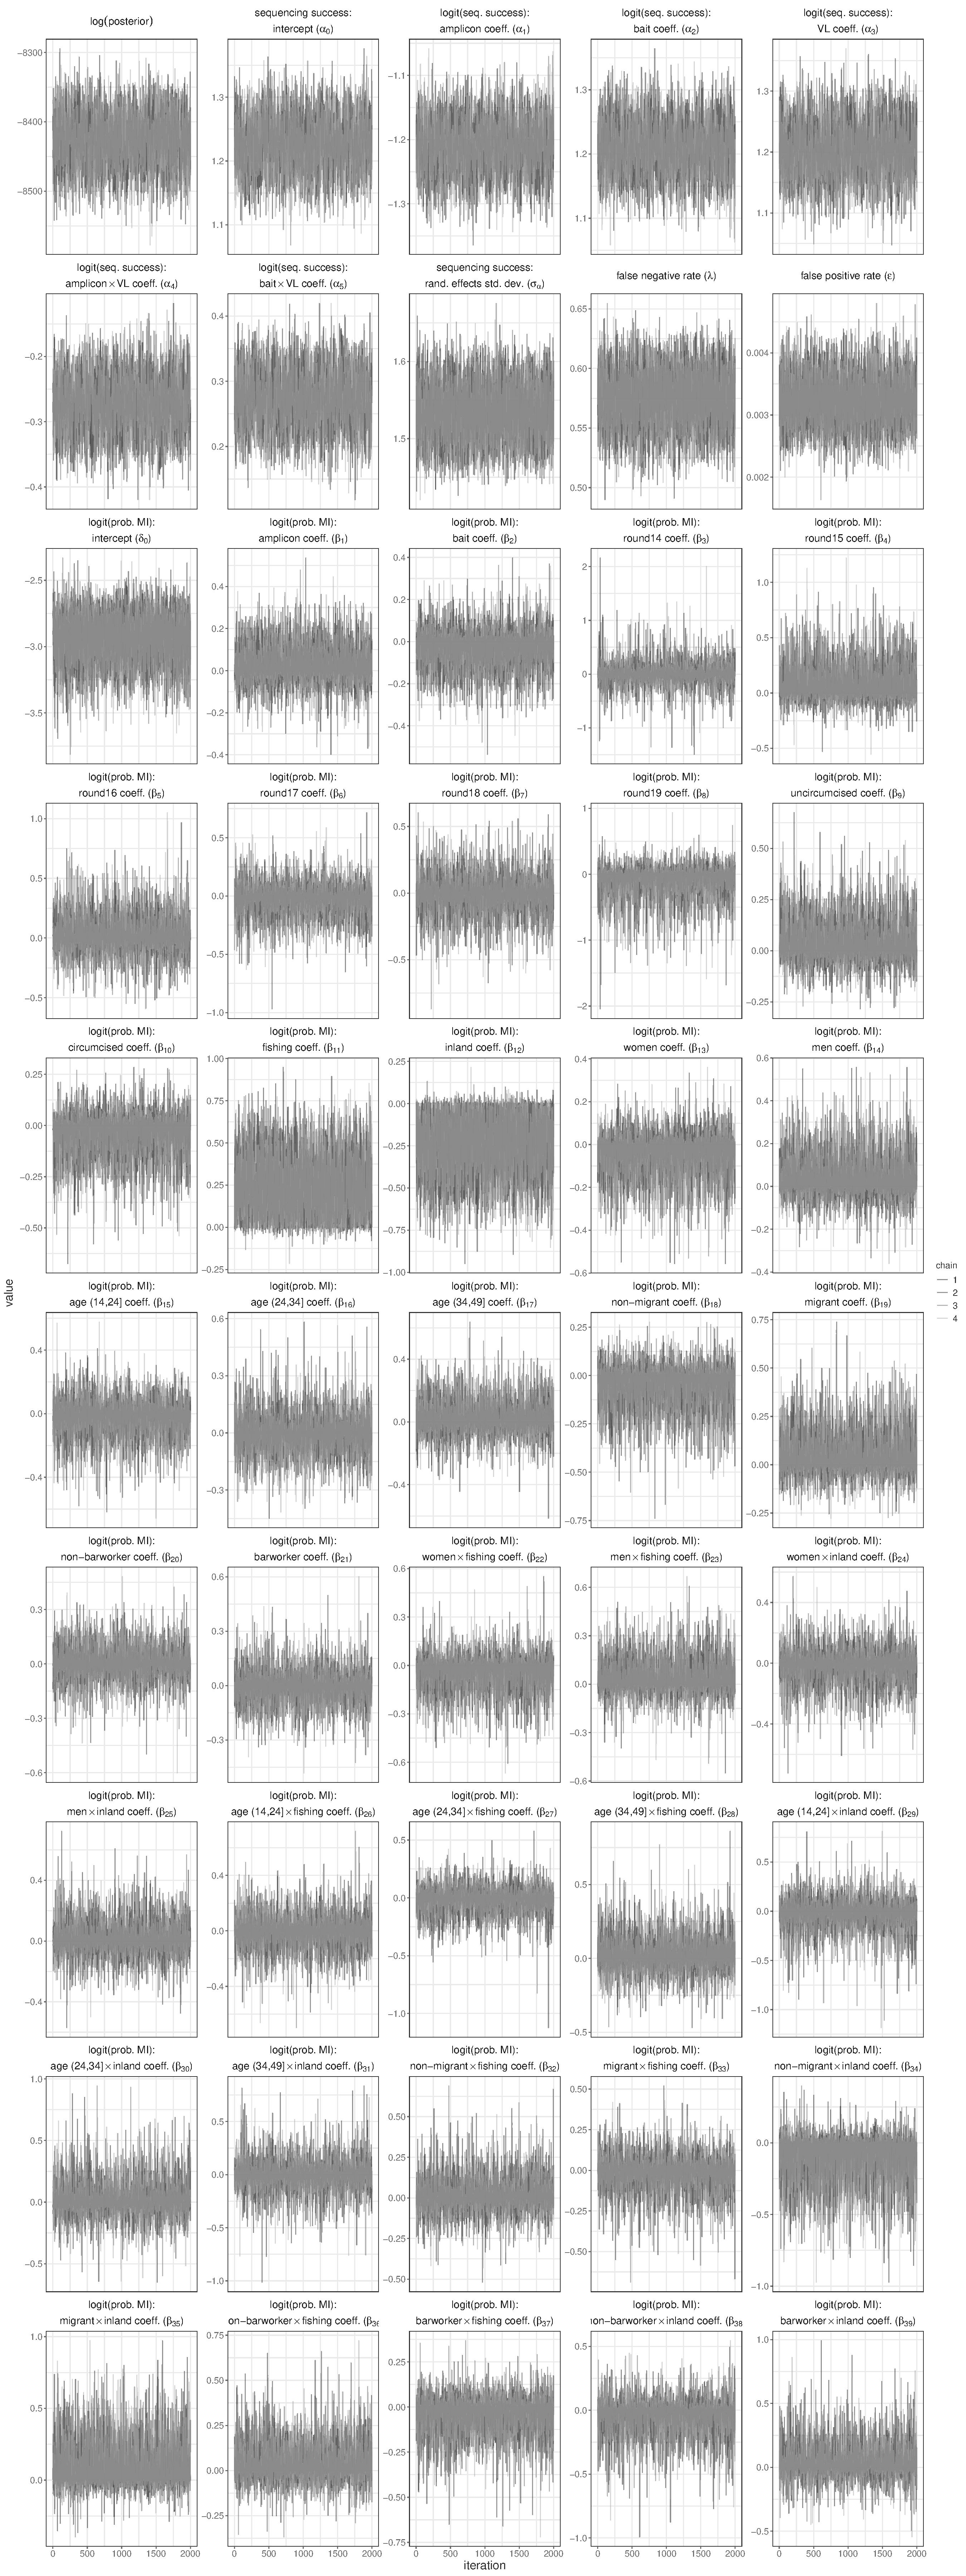
\includegraphics[width=0.7\textwidth]{../../figures/empirical_var_select_trace.pdf}}{}
\caption{{\bf MCMC trace plots for parameters in extended model with variable selection to identify risk factor for harboring multiple infections fit to deep sequence data generated from \protect \var{empirical_var_select_n_participant_visits} Rakai Community Cohort Study participants living with viremic HIV.} Independent chains are shown in shades of grey. Warm-up iterations are excluded. MI = multiple infection. VL = viral load (log\textsubscript{10} copies/mL) standardized to mean = 0 and std. dev = 1. Std. dev. = standard deviation.}
\end{figure}

\begin{figure}[!ht]
 \ifthenelse{\boolean{includefigs}}{\includegraphics[width=1\textwidth]{../../figures/empirical_var_select_pairs.pdf}}{}
\caption{{\bf MCMC pairs plots for parameters in extended model with variable selection to identify risk factor for harboring multiple infections fit to deep sequence data generated from \protect \var{empirical_var_select_n_participant_visits} Rakai Community Cohort Study participants living with viremic HIV.} Independent chains are shown in shades of grey. Warm-up iterations are excluded. Includes a sample of 250 iterations per chain. MI = multiple infection. }
\end{figure}

\begin{figure}[!ht]
 \ifthenelse{\boolean{includefigs}}{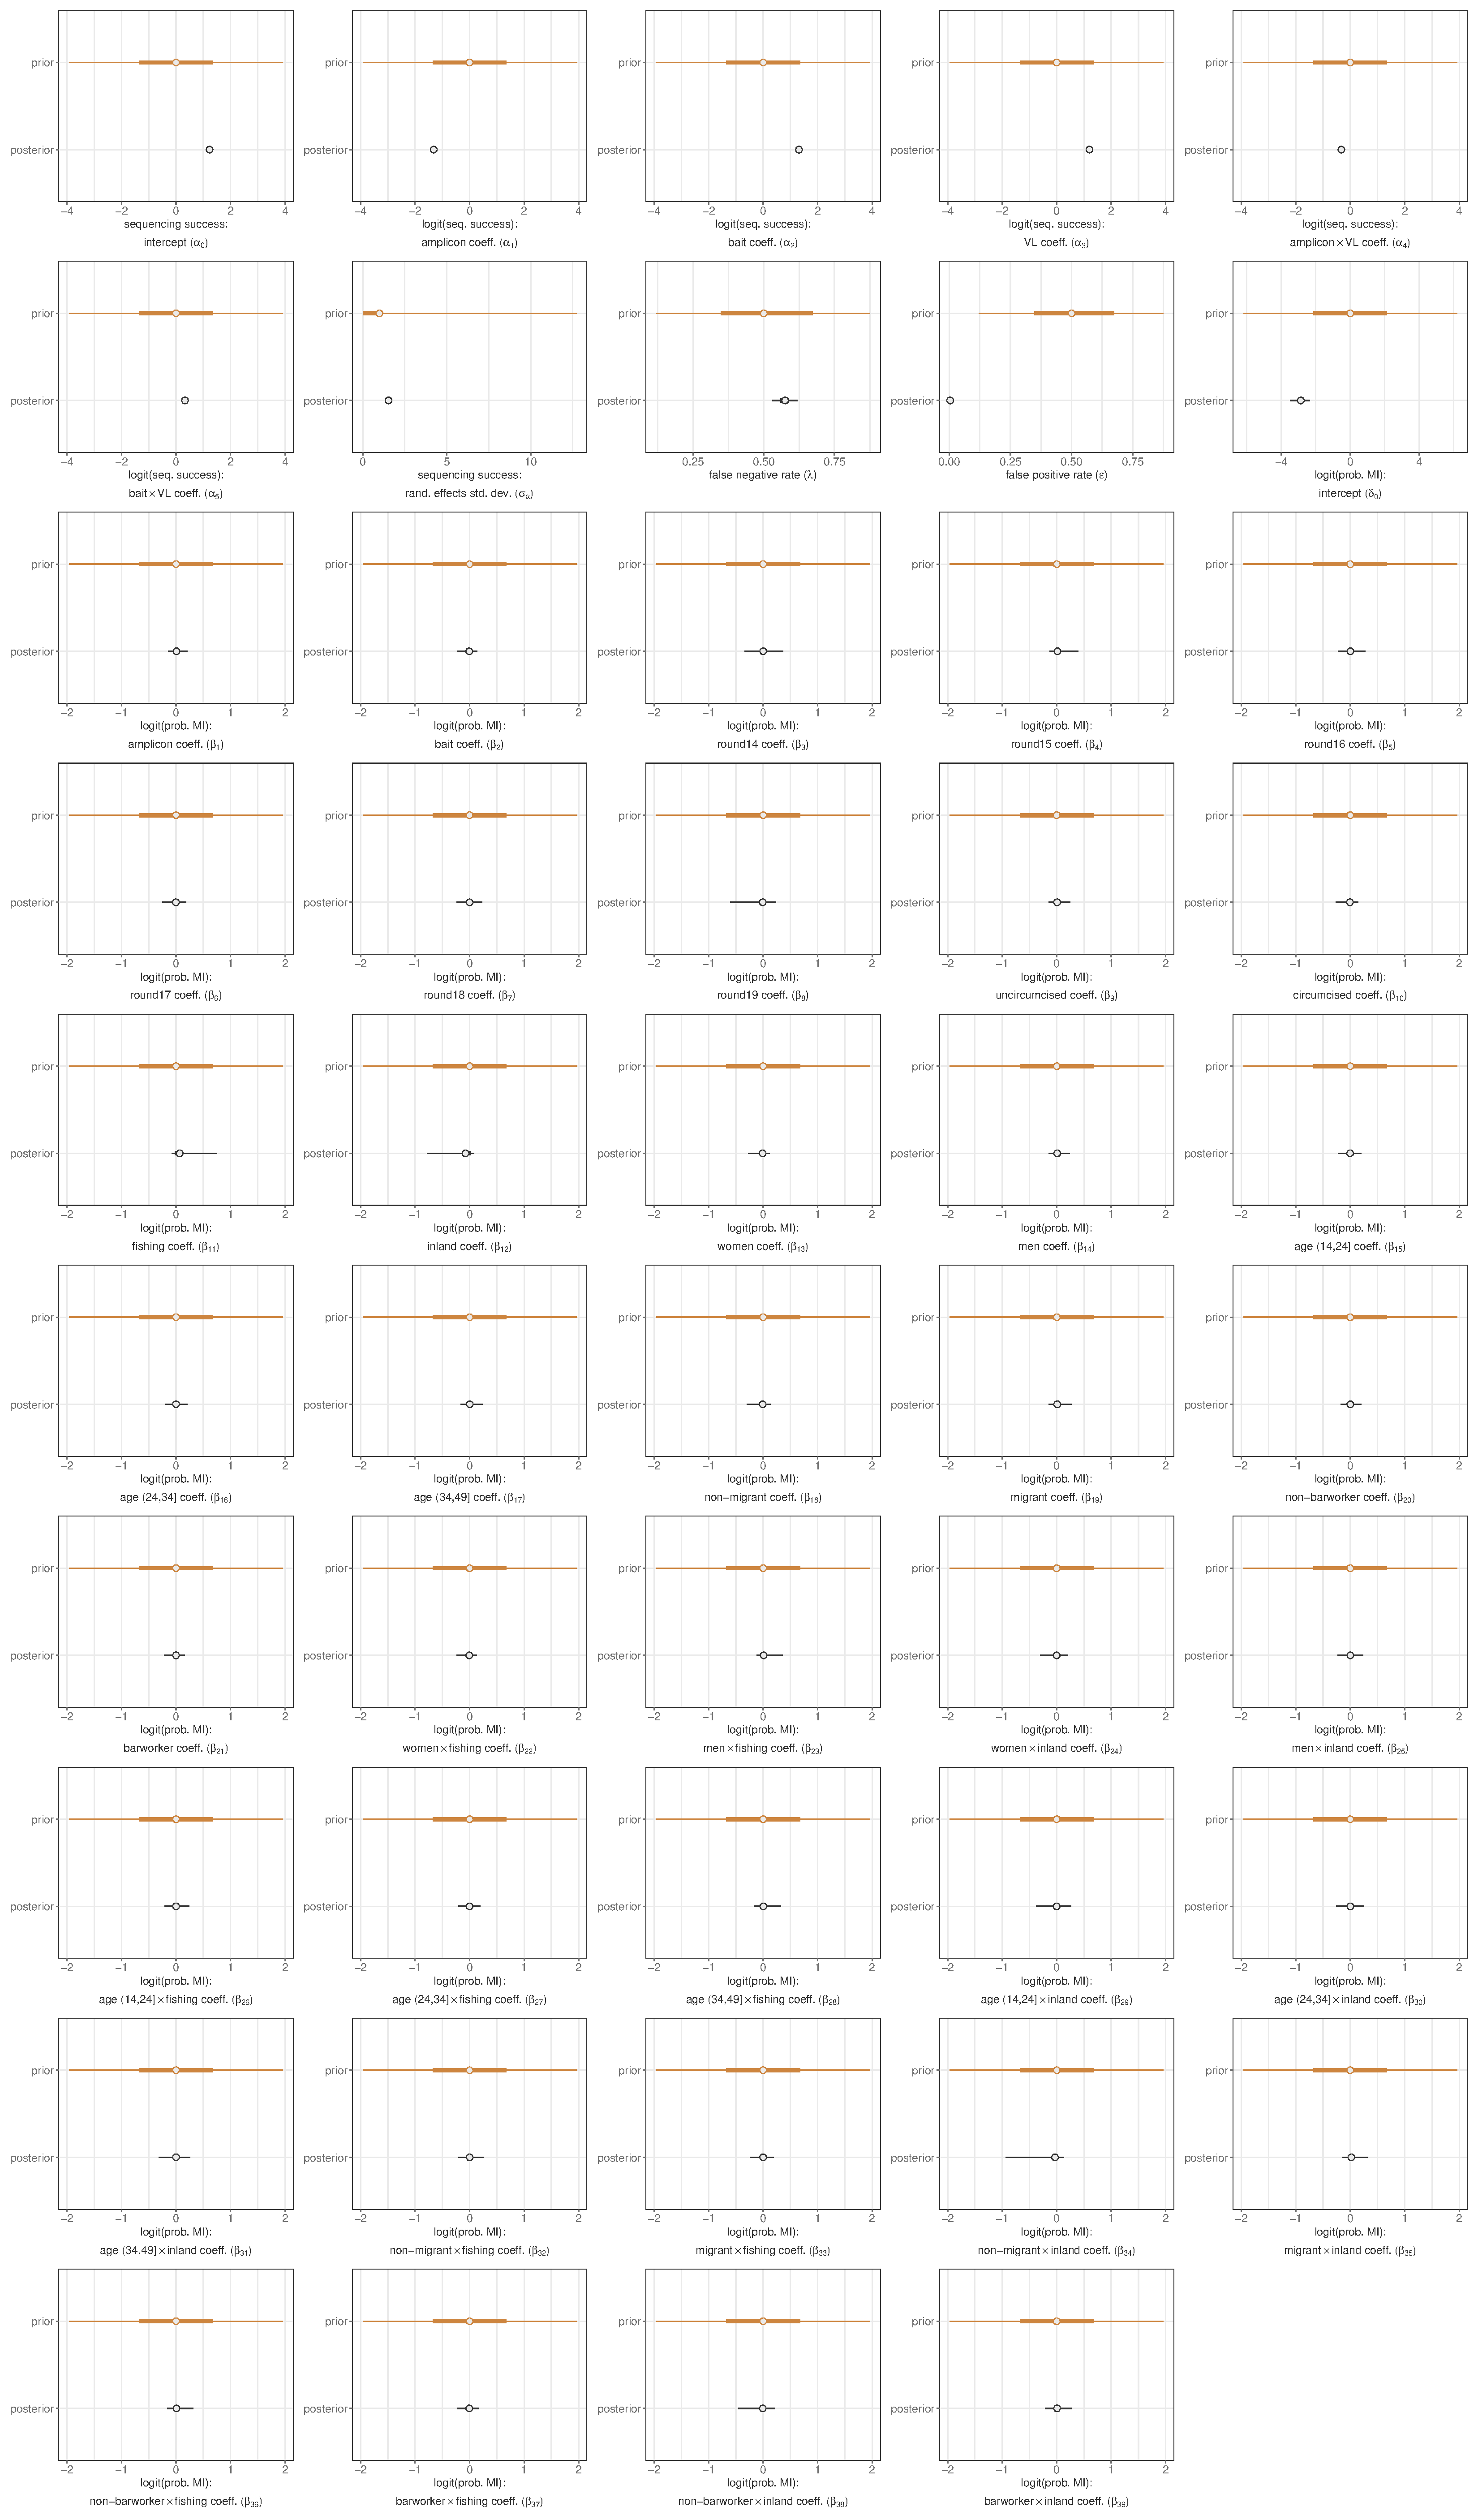
\includegraphics[width=1\textwidth]{../../figures/empirical_var_select_prior.pdf}}{}
\caption{{\bf Comparison of posterior and prior distributions of parameters in extended model with variable selection to identify risk factor fit to deep sequence data generated from \protect \var{empirical_var_select_n_participant_visits} Rakai Community Cohort Study participants living with viremic HIV.} Median is plotted as the central estimate and horizontal bars extend to the 95\% and 50\% HPD. Some horizontal bars do not extend beyond the central point. Warm-up iterations are excluded. MI = multiple infection. VL = viral load (log\textsubscript{10} copies/mL) standardized to mean = 0 and std. dev = 1. Std. dev. = standard deviation. }
\end{figure}

\end{document}